% ==============================================================================
% Modelo para Especificação de Projeto de Software
% Prof. Vítor E. Silva Souza - NEMO/UFES :: DI/UFES :: PPGI/UFES
%
% Baseado em abtex2-modelo-trabalho-academico.tex, v-1.9.2 laurocesar
% Copyright 2012-2014 by abnTeX2 group at http://abntex2.googlecode.com/ 
%
% This work may be distributed and/or modified under the conditions of the LaTeX 
% Project Public License, either version 1.3 of this license or (at your option) 
% any later version. The latest version of this license is in
% http://www.latex-project.org/lppl.txt.
%
% IMPORTANTE:
% Instruções encontram-se espalhadas pelo documento. Para facilitar sua leitura,
% tais instruções são precedidas por (*) -- utilize a função localizar do seu
% editor para passar por todas elas.
% ==============================================================================

% Usa o estilo abntex2, configurando detalhes de formatação e hifenização.
\documentclass[
	12pt,				
	oneside,		
	a4paper,			
	english,			% Idioma adicional para hifenização.
	french,				% Idioma adicional para hifenização.
	spanish,			% Idioma adicional para hifenização.
	brazil				% O último idioma é o principal do documento.
	]{abntex2}


%%% Importação de pacotes. %%%

% Conserta o erro "No room for a new \count". 
% O comando \reserveinserts deve ser comentado ou não, dependendo da versão do LaTeX.
\usepackage{etex}
%\reserveinserts{28}

% Usa a fonte Latin Modern.
\usepackage{lmodern}

% Seleção de códigos de fonte.
\usepackage[T1]{fontenc}

% Codificação do documento em Unicode.
\usepackage[utf8]{inputenc}

% Usado pela ficha catalográfica.
\usepackage{lastpage}

% Indenta o primeiro parágrafo de cada seção.
\usepackage{indentfirst}

% Controle das cores.
\usepackage[usenames,dvipsnames]{xcolor}
\usepackage{colortbl}

% Inclusão de gráficos.
\usepackage{graphicx}

% \FloatBarrier: impede que figuras flutuem para depois do início da seção seguinte
% (usado nas seções do capítulo de interação humano-computador).
\usepackage{placeins}

% Tabularx package: melhor controle de leiaute de tabelas.
\usepackage{tabularx}

% Longtable package: tabelas que passam do limite de uma página.
\usepackage{longtable}
\usepackage{pdflscape}

% Inclusão de páginas em PDF diretamente no documento (para uso nos apêndices).
\usepackage{pdfpages}

% Para melhorias de justificação.
\usepackage{microtype}

% Citações padrão ABNT.
\usepackage[brazilian,hyperpageref]{backref}
\usepackage[alf]{abntex2cite}	
\renewcommand{\backrefpagesname}{Citado na(s) página(s):~}		% Usado sem a opção hyperpageref de backref.
\renewcommand{\backref}{}										% Texto padrão antes do número das páginas.
\renewcommand*{\backrefalt}[4]{									% Define os textos da citação.
	\ifcase #1
		Nenhuma citação no texto.
	\or
		Citado na página #2.
	\else
		Citado #1 vezes nas páginas #2.
	\fi}

% \rm is deprecated and should not be used in a LaTeX2e document
% http://tex.stackexchange.com/questions/151897/always-textrm-never-rm-a-counterexample
\renewcommand{\rm}{\textrm}

% Inclusão de símbolos não padrão.
\usepackage{amssymb}
\usepackage{eurosym}

% Para utilizar \eqref para referenciar equações.
\usepackage{amsmath}

% Permite mostrar figuras muito largas em modo paisagem com \begin{sidewaysfigure} ao invés de \begin{figure}.
\usepackage{rotating}

% Permite customizar listas enumeradas/com marcadores.
\usepackage{enumitem}

% Permite inserir hiperlinks com \url{}.
\usepackage{bigfoot}
\usepackage{hyperref}

% Permite usar o comando \hl{} para evidenciar texto com fundo amarelo. Útil para chamar atenção a itens a fazer.
\usepackage{soulutf8}

% Colorinlistoftodos package: to insert colored comments so authors can collaborate on the content.
% (*) Indicar o nome do aluno e substituir o nome do professor se for o caso.
\usepackage[colorinlistoftodos, textwidth=20mm, textsize=footnotesize]{todonotes}
\newcommand{\aluno}[1]{\todo[author=\textbf{Aluno},color=green!30,caption={},inline]{#1}}
\newcommand{\vitor}[1]{\todo[author=\textbf{Vítor},color=red!30,caption={},inline]{#1}}

% Permite inserir espaço em branco condicional (incluído no texto final só se necessário) em macros.
\usepackage{xspace}

% Permite incluir listagens de código com o comando \lstinputlisting{}.
\usepackage{listings}
\usepackage{caption}
\DeclareCaptionFont{white}{\color{white}}
\DeclareCaptionFormat{listing}{\colorbox{gray}{\parbox{\textwidth}{#1#2#3}}}
\captionsetup[lstlisting]{format=listing,labelfont=white,textfont=white}
\renewcommand{\lstlistingname}{Listagem}
\definecolor{mygray}{rgb}{0.5,0.5,0.5}
\lstset{
	basicstyle=\scriptsize,
	breaklines=true,
	numbers=left,
	numbersep=5pt,
	numberstyle=\tiny\color{mygray}, 
	rulecolor=\color{black},
	showstringspaces=false,
	tabsize=2,
    inputencoding=utf8,
    extendedchars=true,
    literate=%
    {é}{{\'{e}}}1
    {è}{{\`{e}}}1
    {ê}{{\^{e}}}1
    {ë}{{\¨{e}}}1
    {É}{{\'{E}}}1
    {Ê}{{\^{E}}}1
    {û}{{\^{u}}}1
    {ù}{{\`{u}}}1
    {â}{{\^{a}}}1
    {à}{{\`{a}}}1
    {á}{{\'{a}}}1
    {ã}{{\~{a}}}1
    {Á}{{\'{A}}}1
    {Â}{{\^{A}}}1
    {Ã}{{\~{A}}}1
    {ç}{{\c{c}}}1
    {Ç}{{\c{C}}}1
    {õ}{{\~{o}}}1
    {ó}{{\'{o}}}1
    {ô}{{\^{o}}}1
    {Õ}{{\~{O}}}1
    {Ó}{{\'{O}}}1
    {Ô}{{\^{O}}}1
    {î}{{\^{i}}}1
    {Î}{{\^{I}}}1
    {í}{{\'{i}}}1
    {Í}{{\~{Í}}}1
}

% Atualização ABNT para referências bibliográficas.
\bibliographystyle{abntex2-alf.bst}




%%% Definição de variáveis. %%%
% (*) Substituir os textos abaixo com as informações apropriadas.
\titulo{Happy Paws}
\local{Vitória, ES}
\data{\the\year}
\instituicao{
	Universidade Federal do Espírito Santo -- UFES
	\par
	Centro Tecnológico
	\par
	Departamento de Informática}
\newcommand{\subtitulo}{Documento de Projeto de Sistema}
\newcommand{\versao}{1.0}

% Define a capa.
\renewcommand{\imprimircapa}{%
	\begin{capa}%
		\center
		
		{\ABNTEXchapterfont\large\subtitulo{}}
		\vfill
		\begin{center}
			\ABNTEXchapterfont\bfseries\LARGE\imprimirtitulo
		\end{center}
		
		\vfill
		\large\imprimirlocal
		\linebreak
		\large\imprimirdata
		\vspace*{1cm}
	\end{capa}
}

% Macros específicas do trabalho.
% (*) Inclua aqui termos que são utilizados muitas vezes e que demandam formatação especial.
% Exemplo: Java com TM (trademark) em superscript.
% Use sempre \xspace para que o LaTeX inclua espaço em branco após a macro somente quando necessário.
\newcommand{\java}{Java\texttrademark\xspace}




%%% Configurações finais de aparência. %%%

% Altera o aspecto de algumas cores.
\definecolor{blue}{RGB}{41,5,195}
\definecolor{lightgray}{gray}{0.9}

% Informações do PDF.
\makeatletter
\hypersetup{
	pdftitle={\@title}, 
	pdfauthor={\@author},
	pdfsubject={\imprimirpreambulo},
	pdfcreator={LaTeX with abnTeX2},
	pdfkeywords={abnt}{latex}{abntex}{abntex2}{trabalho acadêmico}, 
	colorlinks=true,				% Colore os links (ao invés de usar caixas).
	linkcolor=blue,					% Cor dos links.
	citecolor=blue,					% Cor dos links na bibliografia.
	filecolor=magenta,				% Cor dos links de arquivo.
	urlcolor=blue,					% Cor das URLs.
	bookmarksdepth=4
}
\makeatother

% Espaçamentos entre linhas e parágrafos.
\setlength{\parindent}{1.3cm}
\setlength{\parskip}{0.2cm}



%%% Páginas iniciais do documento: capa, folha de rosto, ficha, resumo, tabelas, etc. %%%

% Compila o índice.
\makeindex

% Inicia o documento.
\begin{document}

% Retira espaço extra obsoleto entre as frases.
\frenchspacing

% Inclui o brasão da UFES.
\begin{figure}[h]
  \centering
  
\includegraphics[scale=0.055]{brasao.jpg}
  \label{ppts3}
\end{figure} 

% Capa do trabalho.
\imprimircapa


		
% (*) Incluir as contribuições de cada co-autor do documento.
\begin{center}
	\footnotesize
	{\large\bfseries Contribuíram para esta especificação:}
	
	\vspace{0.5cm}
	\begin{tabular}{|p{55mm}|p{50mm}|p{40mm}|} \hline
		\textbf{Nome} & \textbf{Contato} & \textbf{Contribuições} \\ \hline   
        Bernardo Vargens Broedel & \textsf{bernardo.broedel@edu.ufes.br} & Escrita do documento. \\ \hline  
        Eduardo Capobiango Ferraz & \textsf{eduardo.ferraz@edu.ufes.br} & Escrita do documento. \\ \hline 
        Mateus Biancardi da Silva & \textsf{mateus.silva.16@ufes.br} & Escrita do documento. \\ \hline 
        Miguel Zon Murad & \textsf{miguel.murad@edu.ufes.br} & Escrita do documento. \\ \hline 
        Victor Augusto Fernandes Rangel & \textsf{victor.a.rangel@edu.ufes.br} & Escrita do documento. \\ \hline 
	\end{tabular}
	
	\vspace{1.2cm}

	{\large\bfseries Histórico de alterações:}

	\vspace{0.5cm}
	\begin{tabular}{|p{20mm}|p{22mm}|p{98mm}|} \hline
		\textbf{Versão} & \textbf{Data} & \textbf{Alterações} \\ \hline
		1.0 & 14/09/2026 & T1: descrição geral do sistema, plataforma de desenvolvimento, requisitos não funcionais condutores da arquitetura e arquitetura de software (Capítulos 1 a 4). \\ \hline
		2.0 & 09/10/2026 & T2: projeto da lógica de negócio --- componentes de domínio do problema (CDP) e de gerência de tarefas (CGT) dos três subsistemas. \\ \hline
		3.0 & 30/10/2026 & T3: projeto da interação humano-computador --- organização da Camada de Apresentação, perfis de usuário e táticas de usabilidade, protótipo de alta fidelidade e projeto da Camada de Interface com o Usuário dos três subsistemas. Atualização do CGT (Capítulo 5) com as operações usadas pela Camada de Interface com o Usuário. \\ \hline
	\end{tabular}

	\vspace{1cm}
\end{center}
\newpage



%%% Início da parte de conteúdo do documento. %%%
% Marca o início dos elementos textuais.
\textual

% Inclusão dos capítulos.
% Os capítulos seguem na mesma página (\clearpage desativado), mas o \FloatBarrier
% do pacote placeins continua usando o \clearpage original para descarregar as figuras.
\let\clearpageoriginal\clearpage
\let\FloatBarrieroriginal\FloatBarrier
\renewcommand{\FloatBarrier}{\begingroup\let\clearpage\clearpageoriginal\FloatBarrieroriginal\endgroup}
\begingroup
\let\clearpage\relax
% ==============================================================================
% Projeto de Sistema - Nome do Aluno
% Capítulo 1 - Introdução
% ==============================================================================
\chapter{Introdução}
\label{sec-intro}
\vspace{-1cm}

Este documento apresenta o projeto (\textit{design}) do sistema \emph{\imprimirtitulo}. O sistema tem como propósito gerenciar o ciclo completo de intermediação e contratação de serviços de
passeio para cães, permitindo o cadastro e validação de perfis de tutores, animais e passeadores, a realização de buscas filtradas por geolocalização e especialidade, o agendamento de passeios avulsos ou recorrentes, o monitoramento em tempo real do trajeto via GPS, a comunicação direta entre as partes e a efetivação de pagamentos, avaliações e registros fotográficos das atividades realizadas. 


Além desta introdução, este documento está organizado da seguinte forma: 
	a Seção~\ref{sec-plataforma} apresenta a plataforma de software utilizada na implementação do sistema;
	a Seção~\ref{sec-rnfs} apresenta a especificação dos requisitos não funcionais (atributos de qualidade), definindo as táticas e o tratamento a serem dados aos atributos de qualidade considerados condutores da arquitetura; 
	a Seção~\ref{sec-arquitetura} apresenta a arquitetura de software; 
	a Seção~\ref{sec-logica-negocio} apresenta o projeto da lógica de negócio dos subsistemas, com as componentes de domínio do problema e de gerência de tarefas; por fim, 
	a Seção~\ref{sec-ihc} apresenta o projeto da interação humano-computador, com a organização da Camada de Apresentação, o protótipo de alta fidelidade e o projeto da Camada de Interface com o Usuário.


\vspace*{1.3cm}
% ==============================================================================
% Projeto de Sistema - Nome do Aluno
% Capítulo 2 - Plataforma de Desenvolvimento
% ==============================================================================
\chapter{Plataforma de Desenvolvimento}
\label{sec-plataforma}
\vspace{-1cm}



%=======================================================================================================
%			Tabela de Plataforma de Desenvolvimento e Tecnologias Utilizadas
%=======================================================================================================

Na Tabela~\ref{tabela-plataforma} são listadas as tecnologias utilizadas no desenvolvimento da ferramenta, bem como o propósito de sua utilização.

\begin{footnotesize}
\begin{longtable}{|p{2.5cm}|c|p{5cm}|p{5.5cm}|}
	\caption{Plataforma de Desenvolvimento e Tecnologias Utilizadas.}	
	\label{tabela-plataforma}\\\hline

	\rowcolor{lightgray}
	\textbf{Tecnologia} & \textbf{Versão} & \textbf{Descrição} & \textbf{Propósito} \\\hline 
	\endfirsthead
	\hline
	\rowcolor{lightgray}
	\textbf{Tecnologia} & \textbf{Versão} & \textbf{Descrição} & \textbf{Propósito} \\\hline 
	\endhead
		
	Next.js & 16.3 & Framework React para desenvolvimento web full-stack, com suporte a renderização no servidor (SSR/SSG) e rotas de API integradas & Base do desenvolvimento da aplicação, unificando front-end e back-end em um único projeto \\ \hline
	TypeScript & 7.0 & Superset do JavaScript que adiciona tipagem estática ao código & Garantir maior segurança e manutenibilidade do código, reduzindo erros em tempo de execução \\ \hline
	PostgreSQL & 18.0 & Sistema de gerenciamento de banco de dados relacional (SGBD) open-source & Armazenamento e persistência dos dados da aplicação \\ \hline
	Drizzle ORM & 0.45 & ORM (\textit{Object-Relational Mapper}) leve e \textit{type-safe} para TypeScript & Mediar a comunicação entre a aplicação e o banco PostgreSQL de forma tipada, sem necessidade de SQL manual \\ \hline
	Better Auth & --- & Biblioteca de autenticação para TypeScript que executa dentro da própria aplicação e guarda usuários, sessões e credenciais no banco de dados, com adaptador para o Drizzle ORM & Cadastro e login por e-mail e senha, gerenciamento de sessões, armazenamento seguro das senhas e proteção das telas e \textit{Server Actions} conforme o perfil do usuário (Tutor, Passeador ou Atendente) \\ \hline
	Tailwind CSS & 4.3 & Framework CSS \textit{utility-first} para estilização de interfaces & Estilização rápida e consistente dos componentes visuais do sistema \\ \hline
	shadcn/ui & --- & Coleção de componentes de interface reutilizáveis sobre Radix UI e Tailwind, instalada via CLI & Acelerar o desenvolvimento do front-end com componentes prontos e customizáveis \\ \hline

\end{longtable}
\end{footnotesize}


%=======================================================================================================
%			Tabela de Softwares de Apoio ao Desenvolvimento do Projeto
%=======================================================================================================

Na Tabela~\ref{tabela-software} vemos os softwares que apoiaram o desenvolvimento de documentos e também do código fonte.

\begin{footnotesize}
\begin{longtable}{|p{2.5cm}|c|p{5cm}|p{5.5cm}|}
	\caption{Softwares de Apoio ao Desenvolvimento do Projeto}	
	\label{tabela-software}\\\hline
	
	\rowcolor{lightgray}
	\textbf{Tecnologia} & \textbf{Versão} & \textbf{Descrição} & \textbf{Propósito} \\\hline 
	\endfirsthead
	\hline
	\rowcolor{lightgray}
	\textbf{Tecnologia} & \textbf{Versão} & \textbf{Descrição} & \textbf{Propósito} \\\hline 
	\endhead
		
	WebStorm & 2026.2 & IDE da JetBrains voltada para desenvolvimento JavaScript/TypeScript, com suporte nativo a frameworks como Next.js e React & Escrita, depuração e navegação no código-fonte da aplicação \\ \hline
	Git & 2.55 & Sistema de controle de versão distribuído & Versionamento do código-fonte e rastreamento do histórico de alterações \\ \hline
	GitHub & --- & Plataforma de hospedagem de repositórios Git, com suporte a \textit{pull requests}, \textit{issues} e integração contínua & Hospedagem do repositório remoto e colaboração entre os membros da equipe \\ \hline
	Overleaf (LaTeX) & --- & Plataforma online de edição colaborativa de documentos em LaTeX & Elaboração e formatação da documentação do projeto (como este documento) \\ \hline
	Trello & --- & Ferramenta de gerenciamento de projetos baseada em quadros \textit{Kanban} & Organização, distribuição e acompanhamento das tarefas da equipe \\ \hline
\end{longtable}
\end{footnotesize}
\vspace*{1.3cm}
\chapter{Requisitos Não Funcionais}
\label{sec-rnfs}
\vspace{-1cm}

A Tabela~\ref{tabela-rnfs} apresenta a especificação dos requisitos não funcionais identificados
no Documento de Especificação de Requisitos, os quais foram
considerados condutores da arquitetura.

% Contador para IDs de Requisitos Não Funcionais.
\newcounter{rnfcount}
\renewcommand*\thernfcount{RNF-\arabic{rnfcount}}
\newcommand*\RNF{\refstepcounter{rnfcount}\thernfcount}
\setcounter{rnfcount}{0}

\begin{footnotesize}
\begin{longtable}{|r|p{13cm}|}
	\caption{Especificação de Requisitos Não Funcionais.}
	\label{tabela-rnfs}\\\hline

	% RNF-1 -- Responsividade multiplataforma (RNF01 do ES1).
	\multicolumn{2}{|p{\dimexpr\linewidth-2\tabcolsep-2\arrayrulewidth}|}{\cellcolor{lightgray}\RNF\label{rnf-multiplataforma} -- O sistema deve possuir interface responsiva, operando em dispositivos móveis (Android/iOS) e navegadores web (RNF01 do Documento de Especificação de Requisitos).}\\\hline

	Categoria: & Portabilidade \\\hline

	\parbox[t]{2cm}{\raggedleft Tática /\\Tratamento:} & Camada de abstração de plataforma: o sistema é uma única aplicação web em Next.js, com interface construída com Tailwind CSS (abordagem \textit{mobile-first}) e componentes shadcn/ui, que se adapta ao tamanho da tela e pode ser instalada como aplicativo (PWA) em Android e iOS. O mesmo código atende tutores, passeadores e atendentes, sem versões separadas por plataforma. \\\hline

	Medida: & Quantidade de funcionalidades (\textit{user stories} US01 a US17) que podem ser executadas por completo nos navegadores e nas larguras de tela alvo. \\\hline

	\parbox[t]{2cm}{\raggedleft Critério de\\Aceitação:} & Todas as funcionalidades (US01 a US17) são executadas sem erro e sem rolagem horizontal nas versões atuais do Chrome (Android), do Safari (iOS) e do Chrome e do Firefox (\textit{desktop}), em telas com largura de 360 px ou mais. \\\hline

	% Linha em branco.
	\multicolumn{2}{c}{}\\\hline

	% RNF-2 -- Segurança de dados de pagamento e localização (RNF02 do ES1).
	\multicolumn{2}{|p{\dimexpr\linewidth-2\tabcolsep-2\arrayrulewidth}|}{\cellcolor{lightgray}\RNF\label{rnf-seguranca-dados} -- Dados sensíveis de pagamento e localização devem ser criptografados (RNF02 do Documento de Especificação de Requisitos).}\\\hline

	Categoria: & Segurança \\\hline

	\parbox[t]{2cm}{\raggedleft Tática /\\Tratamento:} & Criptografar dados em trânsito e em repouso e limitar a exposição dos dados: toda a comunicação (páginas, \textit{Server Actions} e canal de eventos em tempo real) usa HTTPS, e o banco PostgreSQL é hospedado com criptografia de armazenamento habilitada. O número completo do cartão de crédito não é armazenado: o processamento é delegado ao provedor de pagamento, por meio da interface \texttt{GatewayPagamento}, e o sistema guarda apenas o identificador da transação e os últimos dígitos do cartão. As coordenadas de GPS (\texttt{RegistroPasseio}) só são entregues, por sessão autenticada, ao tutor e ao passeador do Passeio correspondente. \\\hline

	Medida: & Percentual das requisições da aplicação feitas sobre HTTPS; presença (ou ausência) de números completos de cartão de crédito no banco de dados; criptografia de armazenamento habilitada (ou não) no banco de dados. \\\hline

	\parbox[t]{2cm}{\raggedleft Critério de\\Aceitação:} & 100\% das requisições são feitas sobre HTTPS; nenhum número completo de cartão de crédito é persistido no banco de dados; a criptografia de armazenamento do banco de dados está habilitada; o acesso ao trajeto de um Passeio por usuário que não seja o tutor ou o passeador desse Passeio é recusado. \\\hline

	% Linha em branco.
	\multicolumn{2}{c}{}\\\hline

	% RNF-3 -- Sincronia em tempo real entre Tutor e Passeador (RNF03 do ES1).
	\multicolumn{2}{|p{\dimexpr\linewidth-2\tabcolsep-2\arrayrulewidth}|}{\cellcolor{lightgray}\RNF\label{rnf-tempo-real} -- O sistema deve garantir a atualização de dados em tempo real para garantir a sincronia entre Tutor e Passeador (RNF03 do Documento de Especificação de Requisitos).}\\\hline

	Categoria: & Eficiência \\\hline

	\parbox[t]{2cm}{\raggedleft Tática /\\Tratamento:} & Introduzir um canal de envio de eventos do servidor para o cliente: a posição do passeador durante o monitoramento GPS (US10), as mensagens do chat interno e os alertas de incidente são enviados por \textit{Server-Sent Events} (SSE), implementados por \textit{Route Handlers} do Next.js e acionados pela interface \texttt{NotificadorTempoReal}. O passeador envia suas posições ao servidor por requisição HTTP, e o servidor as repassa ao tutor pelo canal SSE, o que evita o uso de \textit{polling} periódico. Entre instâncias do servidor, os eventos são repassados pelo mecanismo LISTEN/NOTIFY do PostgreSQL. O SSE foi escolhido em lugar do WebSocket por funcionar com os \textit{Route Handlers} sem exigir um servidor customizado. \\\hline

	Medida: & Latência entre a emissão de um evento (por exemplo, uma atualização de posição do passeador) e seu recebimento pelo cliente destinatário (tutor), sob condições normais de rede. \\\hline

	\parbox[t]{2cm}{\raggedleft Critério de\\Aceitação:} & A posição do passeador deve ser refletida no mapa do tutor em, no máximo, 3 segundos após a mudança de posição real, sob condições normais de conectividade (rede móvel 4G ou superior). \\\hline

	% Linha em branco.
	\multicolumn{2}{c}{}\\\hline

	% RNF-4 -- Tempo de primeiro atendimento de suporte (RNF04 do ES1).
	\multicolumn{2}{|p{\dimexpr\linewidth-2\tabcolsep-2\arrayrulewidth}|}{\cellcolor{lightgray}\RNF\label{rnf-tempo-suporte} -- O suporte ao usuário deve realizar o primeiro atendimento em um tempo máximo de 30 minutos (RNF04 do Documento de Especificação de Requisitos).}\\\hline

	Categoria: & Usabilidade \\\hline

	\parbox[t]{2cm}{\raggedleft Tática /\\Tratamento:} & Suportar a iniciativa do sistema (priorização automática): o horário de abertura de cada chamado é registrado e utilizado para calcular o tempo de espera diretamente na consulta que alimenta o painel do atendente, e chamados do tipo ``Emergência'' são automaticamente destacados e ordenados no topo da lista de atendimentos (CA17.2), reduzindo o tempo de triagem manual pela equipe de suporte. \\\hline

	Medida: & Tempo decorrido entre a abertura de um chamado (registro do campo \texttt{dataAbertura} na classe Chamado) e a primeira resposta de um Atendente (\texttt{dataPrimeiraResposta}). \\\hline

	\parbox[t]{2cm}{\raggedleft Critério de\\Aceitação:} & Ao menos 95\% dos chamados devem receber uma primeira resposta do Atendente em até 30 minutos após sua abertura; chamados do tipo ``Emergência'' devem aparecer no topo da lista de atendimentos, independentemente da ordem de chegada. \\\hline

	% Linha em branco.
	\multicolumn{2}{c}{}\\\hline

	% RNF-5 -- Eficiência energética da captura de GPS (RNF05 do ES1).
	\multicolumn{2}{|p{\dimexpr\linewidth-2\tabcolsep-2\arrayrulewidth}|}{\cellcolor{lightgray}\RNF\label{rnf-eficiencia-gps} -- O sistema deve garantir que as coordenadas de GPS sejam atualizadas em segundo plano para economia de energia (RNF05 do Documento de Especificação de Requisitos).}\\\hline

	Categoria: & Eficiência \\\hline

	\parbox[t]{2cm}{\raggedleft Tática /\\Tratamento:} & Gerenciar a demanda de recursos: a captura de coordenadas usa a \textit{Geolocation API} do navegador (\texttt{watchPosition}) somente enquanto o Passeio estiver com status ``iniciado'', com envio ao servidor em intervalo mínimo (por exemplo, a cada 5 segundos, em vez de a cada leitura) e encerramento da captura na conclusão do Passeio. A captura é feita com o aplicativo web aberto (instalado como PWA ou em uma aba do navegador); o rastreamento com a tela bloqueada depende do navegador e é uma limitação conhecida dessa plataforma. \\\hline

	Medida: & Consumo de bateria do dispositivo do passeador atribuível ao rastreamento de GPS, por hora de passeio monitorado, medido em um aparelho de referência. \\\hline

	\parbox[t]{2cm}{\raggedleft Critério de\\Aceitação:} & O rastreamento de GPS não deve consumir mais de 10\% da carga da bateria do aparelho de referência por hora de passeio monitorado, e nenhuma coordenada deve ser capturada fora do intervalo entre o início e o fim de um Passeio. \\\hline

\end{longtable}
\end{footnotesize}
\vspace*{1.3cm}
\chapter{Arquitetura de Software}
\label{sec-arquitetura}
\vspace{-1cm}

A Figura~\ref{figura-arquitetura} mostra a arquitetura do sistema \emph{\imprimirtitulo}.

\begin{figure}[h]
	\centering
	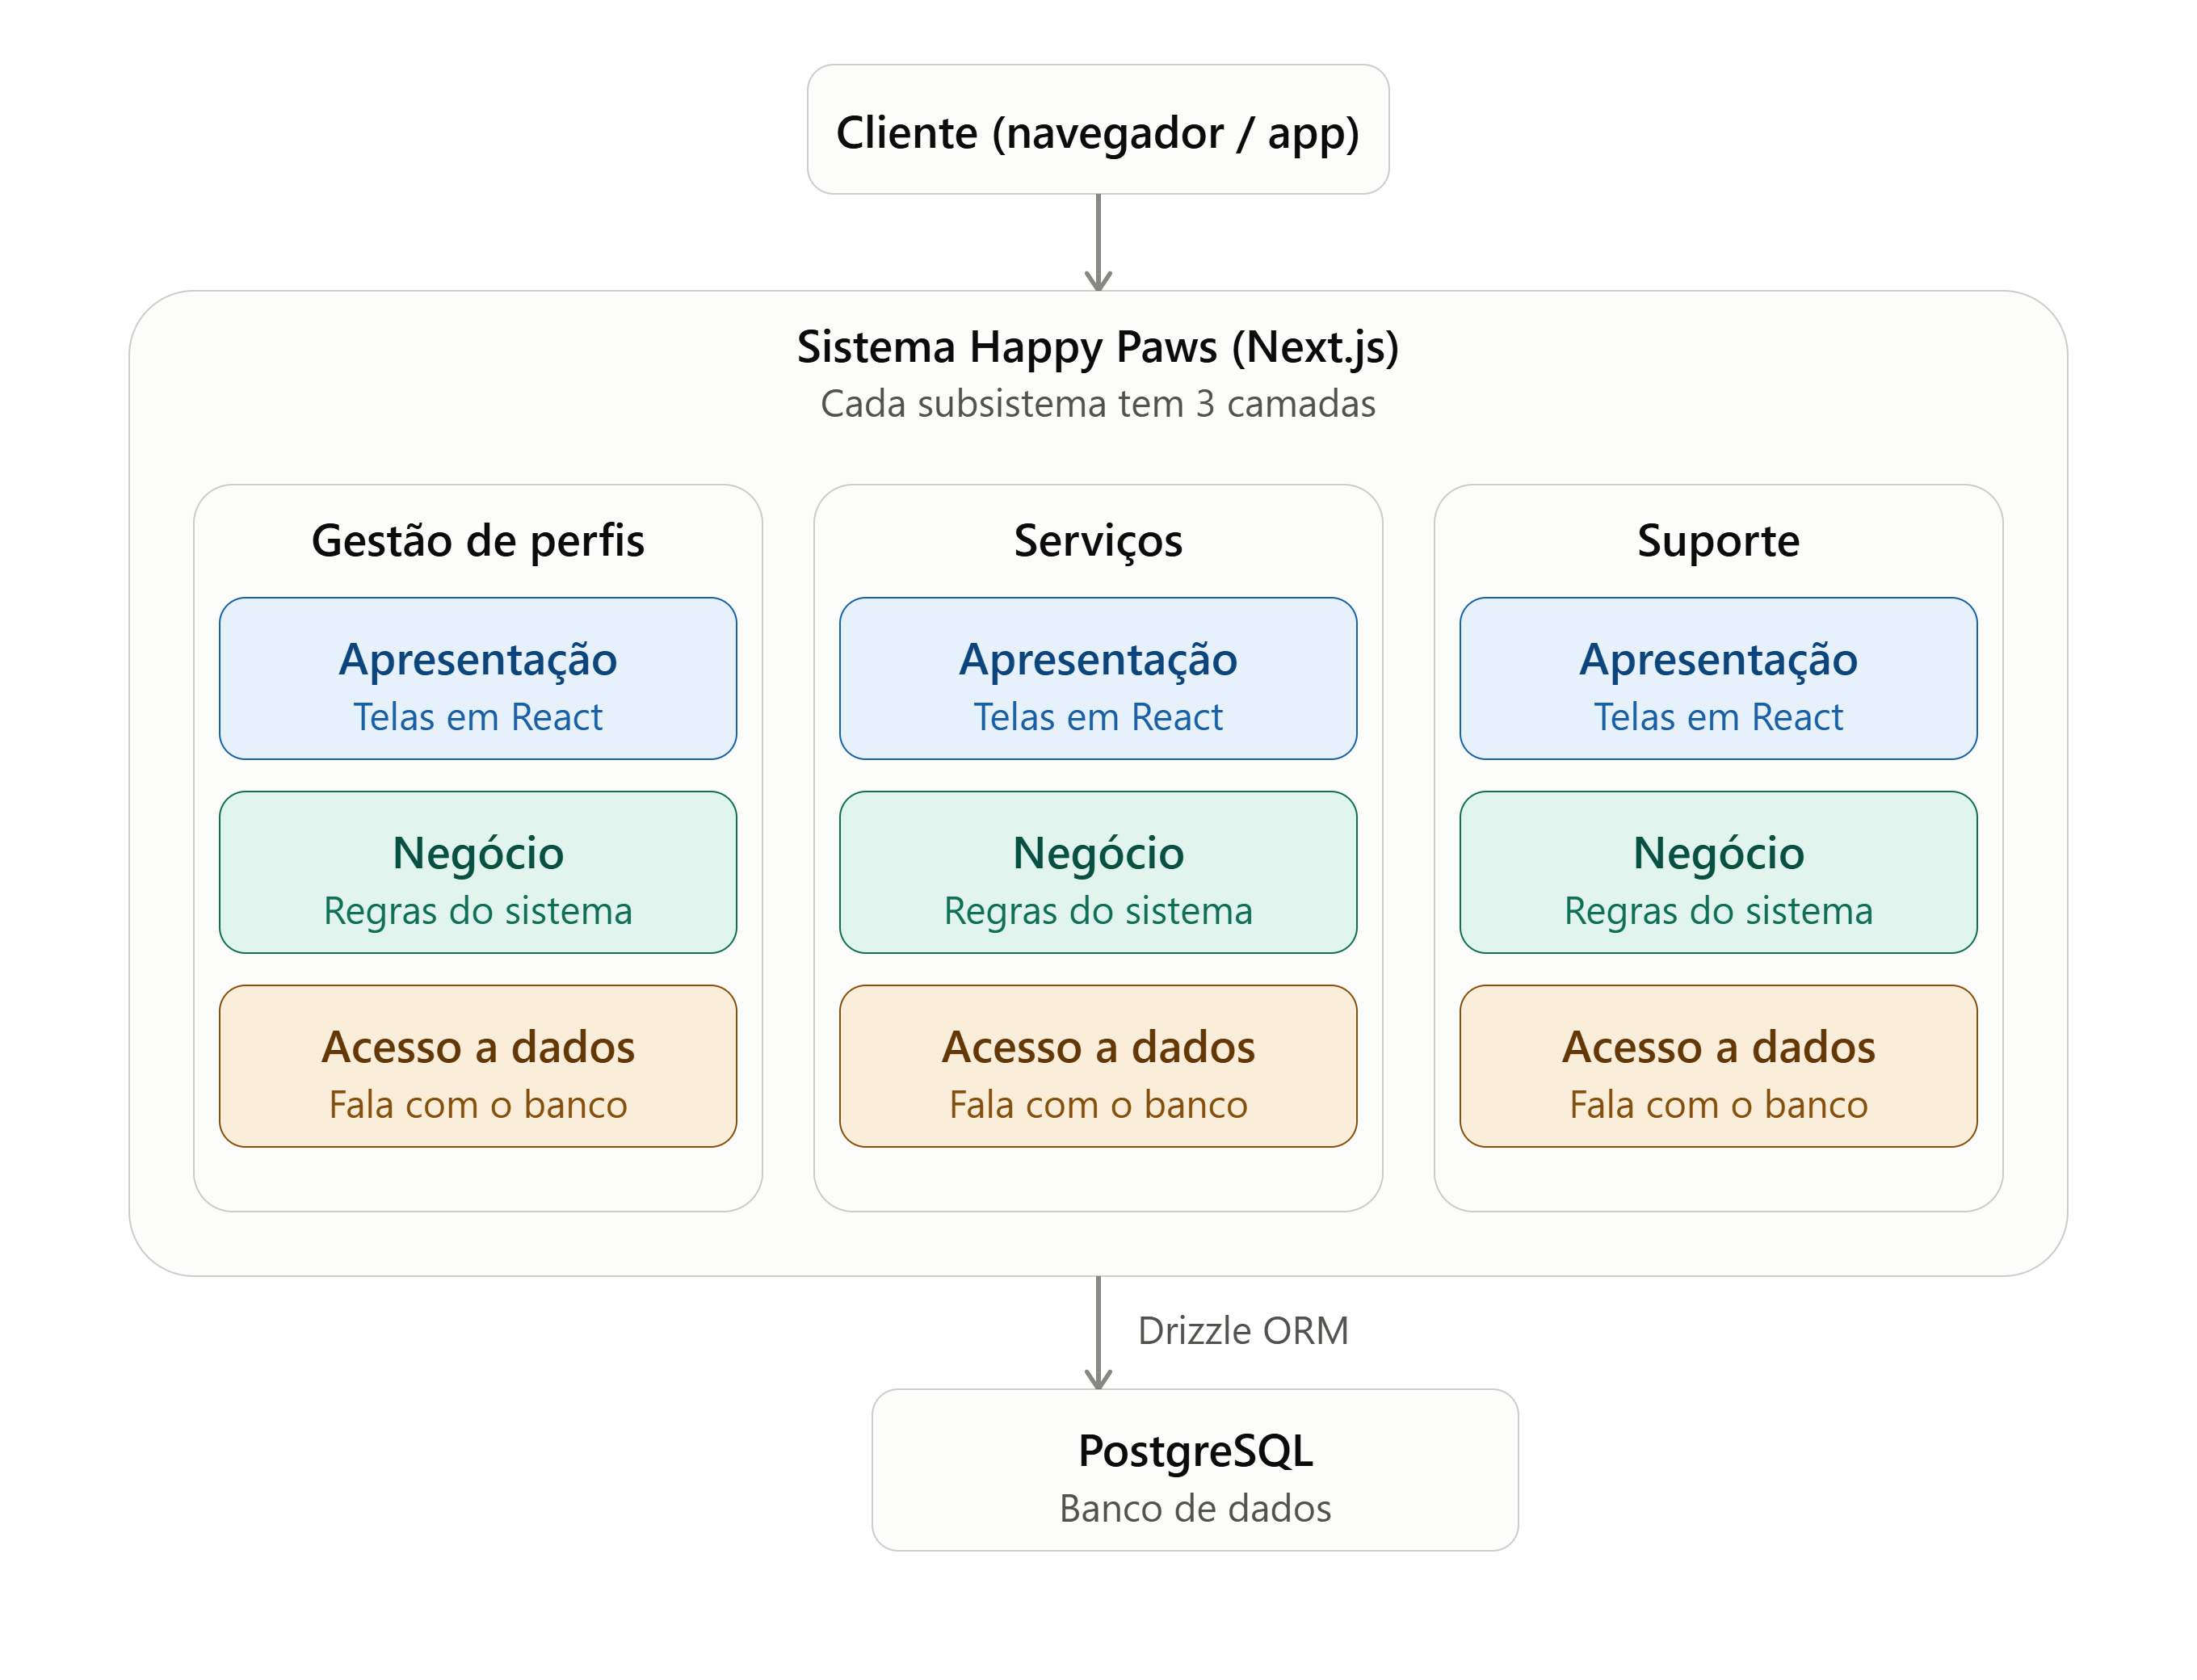
\includegraphics[width=1\textwidth]{figuras/arquitetura_camadas_happy_paws.png}
	\caption{Arquitetura do sistema.}
	\label{figura-arquitetura}
\end{figure}

O sistema Happy Paws usa uma Arquitetura em Camadas~\cite{fowler:book02}. Essa arquitetura é usada nos três subsistemas do sistema: Gestão de Perfis, Serviços e Suporte, como mostra a Figura~\ref{figura-arquitetura}. As camadas são: Apresentação, Negócio e Acesso a Dados.

A camada de Apresentação mostra as telas do sistema e recebe as ações do usuário. Ela é feita com componentes React do Next.js, usando a biblioteca shadcn/ui e o Tailwind CSS para o visual.

A camada de Negócio tem as regras do sistema. Por exemplo, não deixar cadastrar dois usuários com o mesmo CPF, ou não deixar um passeador levar mais cães do que o limite dele. Essa camada é feita com \emph{Server Actions} do Next.js. Ela fica entre a camada de Apresentação e a camada de Acesso a Dados.

A camada de Acesso a Dados fala com o banco de dados. Ela guarda, busca, atualiza e apaga as informações do sistema no PostgreSQL, usando o Drizzle ORM.
\vspace*{1.3cm}
% O capítulo ch5-componentes foi substituído pelos capítulos de lógica de negócio
% (T2) e de interação humano-computador (T3), que tratam das mesmas componentes com
% mais detalhe. O arquivo foi mantido na pasta apenas como histórico.
%\chapter{Projeto dos Componentes da Arquitetura}
\label{sec-componentes}
\vspace{-1cm}

% Permite quebrar melhor os parágrafos com identificadores longos em fonte monoespaçada.
\emergencystretch=3em

Como mostra a Figura~\ref{figura-arquitetura}, o sistema Happy Paws tem três subsistemas: Gestão de Perfis, Serviços e Suporte. Cada um deles é dividido em três camadas: Apresentação, Negócio e Acesso a Dados. Nas seções seguintes, cada subsistema é detalhado, mostrando os modelos de projeto de cada camada.

Na Camada de Negócio, cada subsistema é dividido em dois pacotes, que correspondem às componentes descritas por Falbo~\cite{falbo:notas18}, conforme a Tabela~\ref{tabela-pacotes}: o pacote \texttt{cdp}, com a Componente de Domínio do Problema (CDP), que contém as classes que representam os elementos do domínio e foram identificadas nos modelos estruturais da fase de requisitos; e o pacote \texttt{cgt}, com a Componente de Gerência de Tarefas (CGT), que contém as classes de aplicação (prefixo \texttt{Apl}) que implementam as funcionalidades representadas nas \textit{user stories}. As classes de aplicação são o ponto de entrada da Camada de Negócio e são chamadas pelas \emph{Server Actions} do Next.js, que desempenham o papel de controladoras na Camada de Apresentação.

\begin{footnotesize}
\begin{longtable}{|c|c|}
	\caption{Pacotes da Camada de Negócio e as componentes equivalentes em~\cite{falbo:notas18}.}
	\label{tabela-pacotes}\\\hline
	\rowcolor{lightgray}
	\textbf{Pacote} & \textbf{Componente} \\\hline
	\endfirsthead
	\hline
	\rowcolor{lightgray}
	\textbf{Pacote} & \textbf{Componente} \\\hline
	\endhead
	\texttt{cdp} & Componente de Domínio do Problema (CDP) \\\hline
	\texttt{cgt} & Componente de Gerência de Tarefas (CGT) \\\hline
\end{longtable}
\end{footnotesize}

A Figura~\ref{figura-pacotes} mostra os pacotes da Camada de Negócio e suas dependências. Dentro de cada subsistema, o pacote \texttt{cgt} depende do pacote \texttt{cdp}, que não conhece a aplicação. Entre subsistemas, tanto Serviços quanto Suporte dependem de Gestão de Perfis (seus elementos referenciam Tutor, Passeador, Cachorro, Usuário e Atendente), e Suporte depende também de Serviços, pois um Chamado pode se referir a um Passeio. Além disso, Serviços e Suporte dependem do pacote \texttt{Comum}, que contém a interface \texttt{NotificadorTempoReal}, usada para enviar notificações e eventos em tempo real aos usuários e implementada na infraestrutura do sistema por meio de \textit{Server-Sent Events} (SSE) servidos por \textit{Route Handlers} do Next.js, com o mecanismo LISTEN/NOTIFY do PostgreSQL para repassar os eventos entre instâncias do servidor (RNF-3).

\begin{figure}[h]
	\centering
	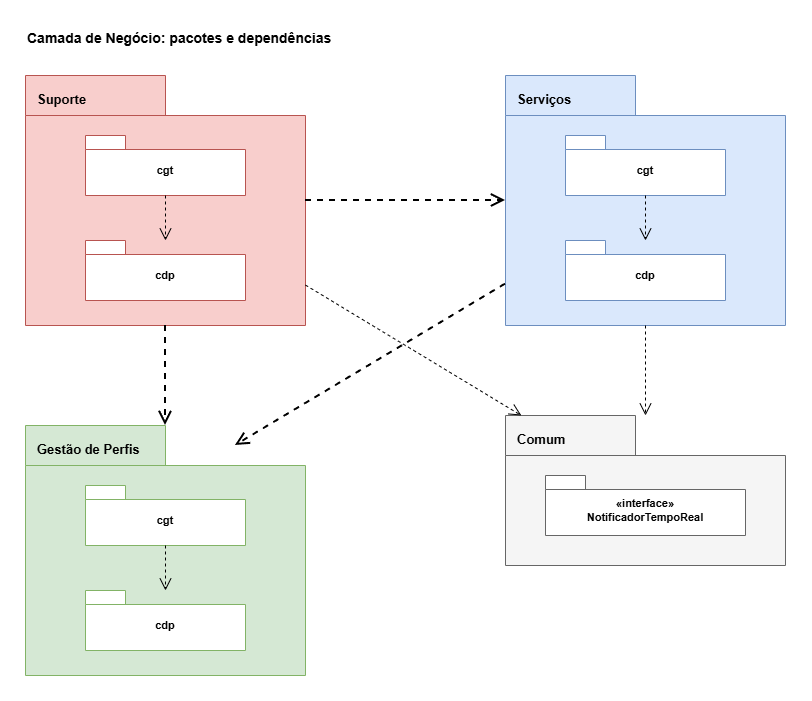
\includegraphics[width=1\textwidth,height=0.7\textheight,keepaspectratio]{figuras/ln-pacotes.png}
	\caption{Pacotes da Camada de Negócio e suas dependências.}
	\label{figura-pacotes}
\end{figure}


%=======================================================================================================
\section{Subsistema Gestão de Perfis}
\label{sec-componentes-perfis}

O subsistema Gestão de Perfis cuida do cadastro de tutores, cães e passeadores. Ele também cuida da validação de identidade dos passeadores e do compartilhamento de perfis de cães entre tutores (US01 a US06).


\subsection{Camada de Negócio}
\label{sec-componentes-perfis-negocio}

A Figura~\ref{figura-perfis-cdp} mostra o projeto da Componente de Domínio do Problema (pacote \texttt{cdp}) do subsistema Gestão de Perfis, obtido a partir do diagrama de classes do Documento de Especificação de Requisitos (Figura 35).

\begin{figure}[h]
	\centering
	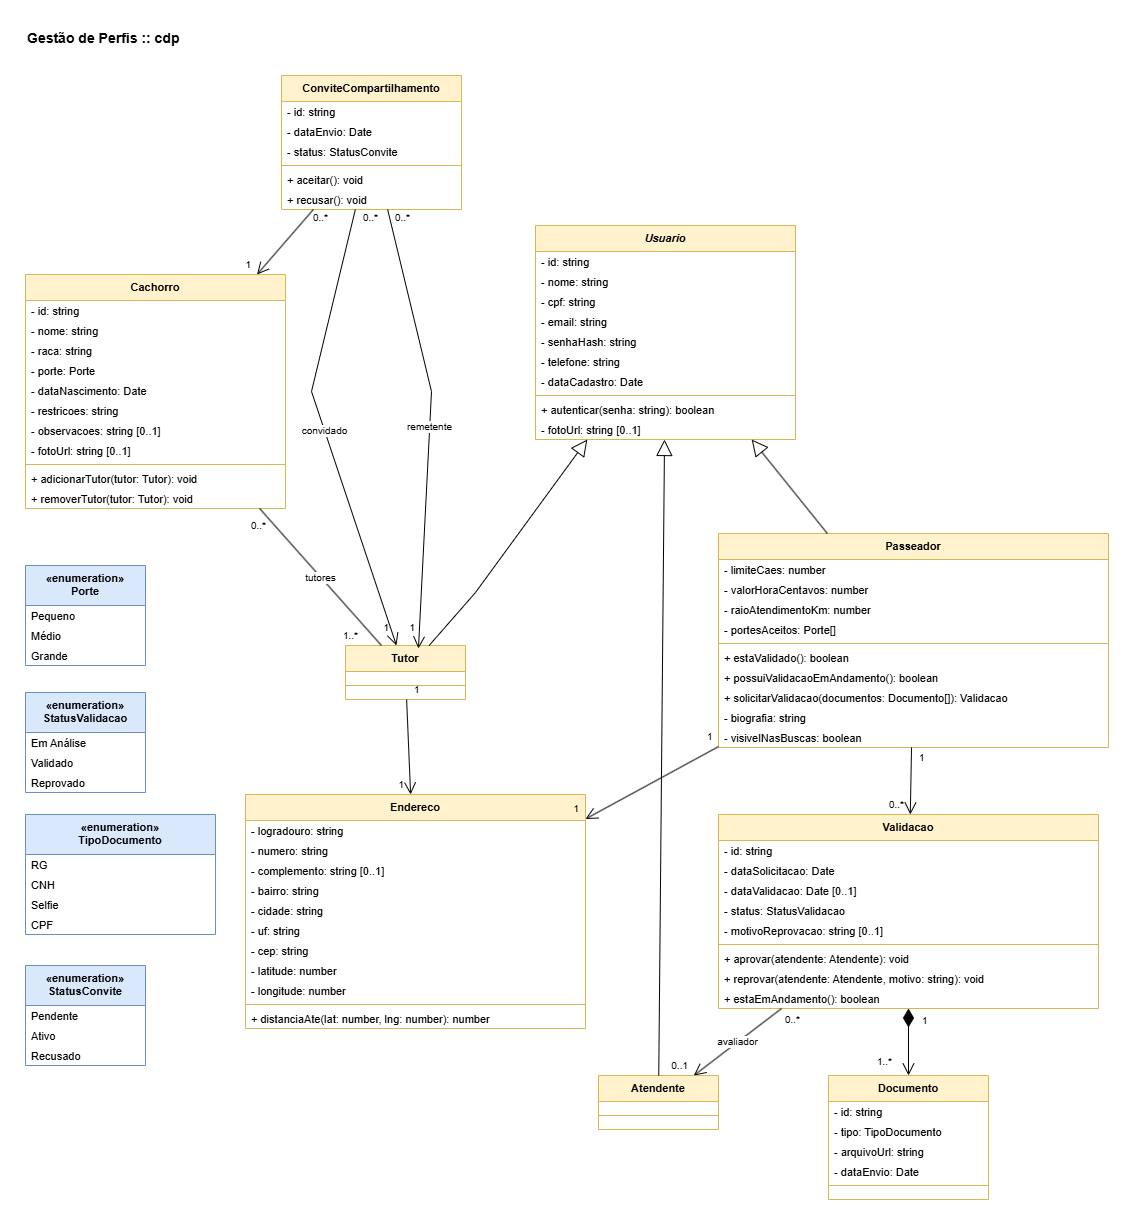
\includegraphics[width=1\textwidth,height=0.85\textheight,keepaspectratio]{figuras/ln-perfis-cdp.png}
	\caption{Projeto da Componente de Domínio do Problema (\texttt{cdp}) do subsistema Gestão de Perfis.}
	\label{figura-perfis-cdp}
\end{figure}

As principais decisões que levaram a este modelo, em relação ao modelo de requisitos, foram:

\begin{itemize}
	\item \textbf{Generalização de Pessoa em Usuário.} A classe abstrata \texttt{Pessoa} do modelo de requisitos foi renomeada para \texttt{Usuario}, generalizando Tutor, Passeador e Atendente. Foram acrescentados \texttt{senhaHash}, \texttt{dataCadastro} e a operação \texttt{autenticar()}, necessários para o acesso ao sistema, e o atributo \texttt{fotoUrl}, que corresponde à foto de perfil das telas de cadastro. A autenticação é feita pela biblioteca Better Auth (Capítulo~\ref{sec-plataforma}): \texttt{senhaHash} e \texttt{autenticar()} representam, no CDP, a credencial do usuário, mas o hash da senha é calculado e guardado pela própria biblioteca, em sua tabela de contas, e a operação \texttt{AplCadastroUsuario.autenticar()} apenas delega a ela a verificação, de modo que o código do sistema nunca calcula nem compara hashes de senha. Como o Drizzle ORM não oferece herança de entidades, a generalização é realizada no banco de dados por uma tabela comum de usuários, referenciada por chave estrangeira pelas tabelas de cada papel.

	\item \textbf{Criação da classe Validação.} No modelo de requisitos, o estado da validação era o atributo \texttt{status} de Passeador, mas as restrições RI-4 (um Passeador não pode ter mais de uma Validação ao mesmo tempo) e RI-5 (a data de envio dos Documentos deve ser anterior ou igual à data de conclusão da Validação) já tratavam a Validação como um conceito próprio. Foi criada, então, a classe \texttt{Validacao}, com os atributos \texttt{dataSolicitacao}, \texttt{dataValidacao}, \texttt{status} e \texttt{motivoReprovacao} (este exigido pelo CA04.4), associada a um Passeador (que passa a ter um histórico de validações), a seus Documentos (composição) e ao Atendente que a avaliou. O \texttt{status} deixou de ser atributo de Passeador, que passa a obter essa informação por meio da operação \texttt{estaValidado()}.

	\item \textbf{Criação da classe ConviteCompartilhamento.} O compartilhamento de perfil de um cão entre tutores (US05) possui estado próprio (pendente até o aceite, ativo depois do aceite, CA05.2 e CA05.3) e envolve três participantes: o cão, o tutor que convida (\texttt{remetente}) e o tutor convidado (\texttt{convidado}). Por isso, foi criada a classe \texttt{ConviteCompartilhamento}, com as operações \texttt{aceitar()} e \texttt{recusar()}. A associação entre Cachorro e Tutor permanece muitos-para-muitos, com a cardinalidade mínima 1 do lado do Tutor, que garante a RI-3.

	\item \textbf{Atributos do Passeador.} Foram acrescentados \texttt{biografia} (CA03.1), \texttt{portesAceitos} (campo ``Porte aceito'' da tela de cadastro, usado como filtro na busca, CA07.1) e \texttt{visivelNasBuscas} (controle de disponibilidade da tela de modo de trabalho, CA06.4). O preço por hora passou a ser armazenado em centavos (\texttt{valorHoraCentavos}), evitando erros de arredondamento com números de ponto flutuante. O atributo \texttt{raioAtendimentoKm} apoia a busca por geolocalização citada no propósito do sistema.

	\item \textbf{Atributos de Endereço e de Cachorro.} Endereço ganhou \texttt{latitude} e \texttt{longitude} e a operação \texttt{distanciaAte()}, que permitem filtrar passeadores por proximidade. Em Cachorro, a idade foi substituída por \texttt{dataNascimento} (a idade é calculada), e foram mantidos \texttt{restricoes} (alergias e medos, CA02.1) e \texttt{observacoes} (campo livre da tela de cadastro).

	\item \textbf{Enumerações.} Os valores das enumerações seguem os nomes dos critérios de aceitação do documento de requisitos: \texttt{StatusValidacao} (Em Análise, Validado, Reprovado), \texttt{StatusConvite} (Pendente, Ativo, Recusado, este último introduzido pela operação \texttt{recusar()}) e \texttt{TipoDocumento} (RG, CNH, Selfie, CPF).
\end{itemize}

A Figura~\ref{figura-perfis-cgt} mostra o projeto da Componente de Gerência de Tarefas (pacote \texttt{cgt}) do subsistema, que depende das classes do pacote \texttt{cdp}. Cada classe de aplicação agrupa as operações de um conjunto de \textit{user stories}:

\begin{figure}[h]
	\centering
	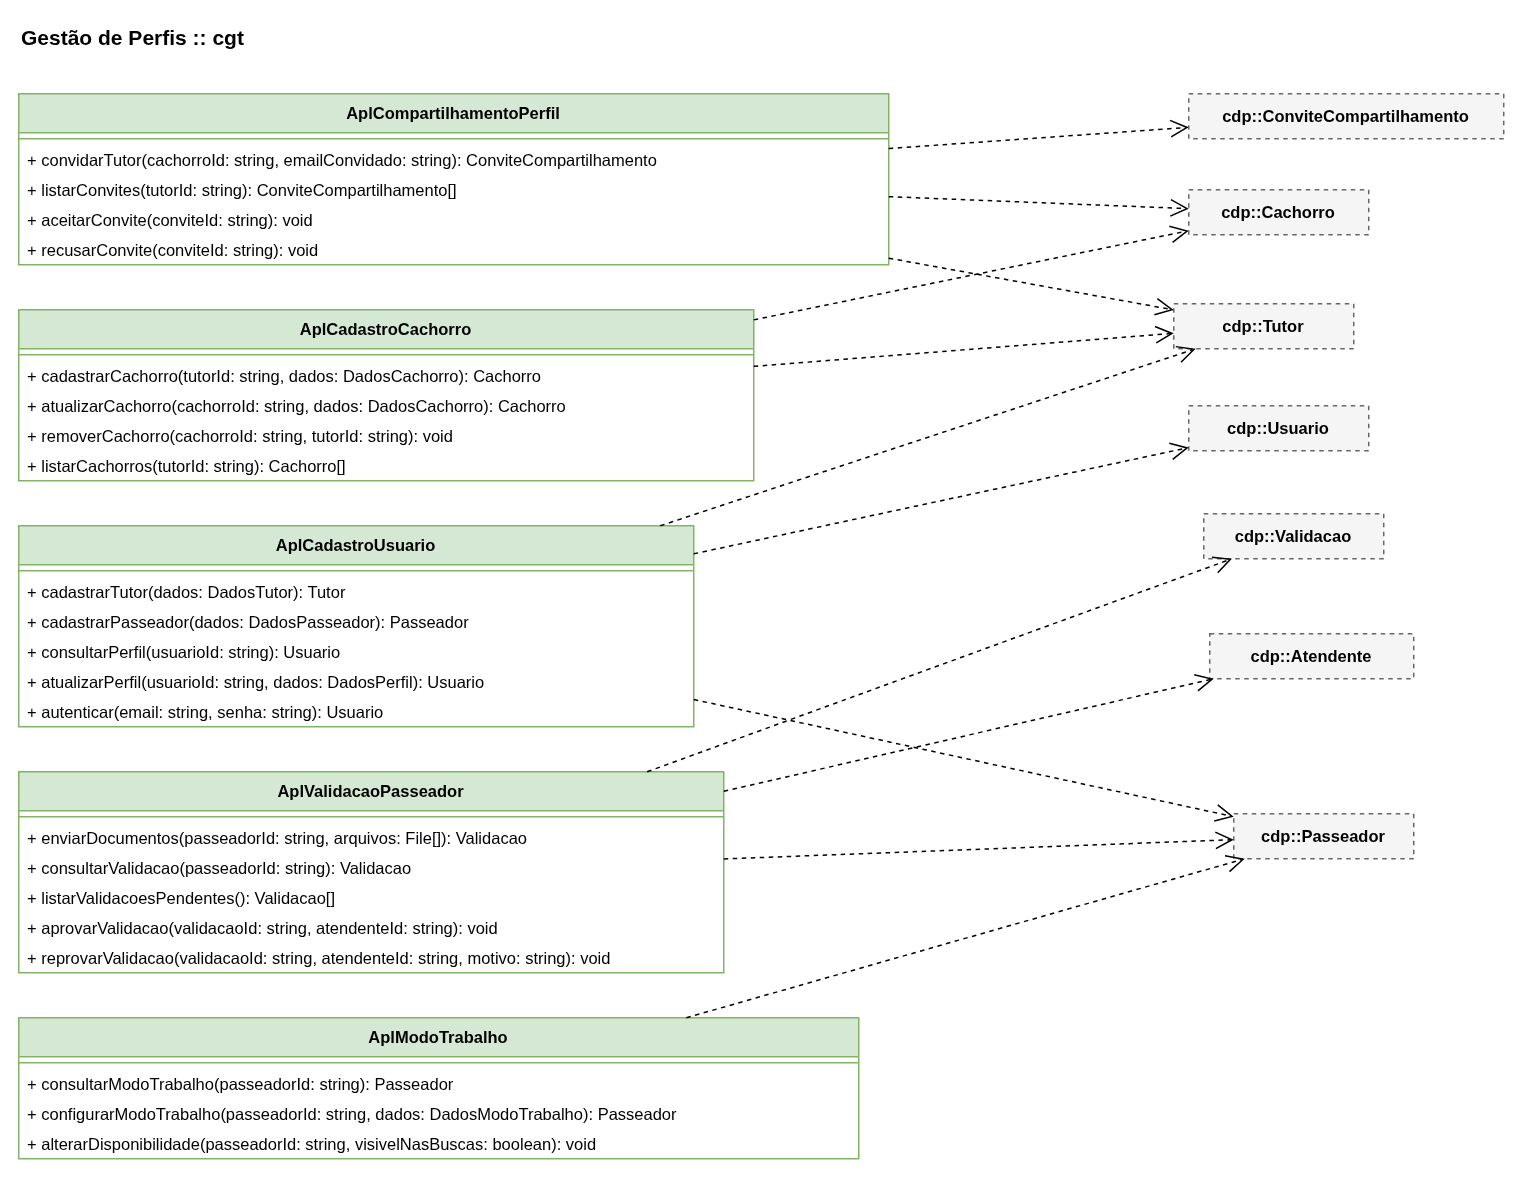
\includegraphics[width=1\textwidth,height=0.85\textheight,keepaspectratio]{figuras/ln-perfis-cgt.png}
	\caption{Projeto da Componente de Gerência de Tarefas (\texttt{cgt}) do subsistema Gestão de Perfis.}
	\label{figura-perfis-cgt}
\end{figure}

\begin{itemize}
	\item \texttt{AplCadastroUsuario}: cadastro de Tutor e de Passeador, atualização de perfil e autenticação (US01, US03). Verifica a unicidade de CPF e e-mail (RI-1 e RI-2);
	\item \texttt{AplCadastroCachorro}: cadastro, atualização, remoção e listagem de cães de um Tutor (US02). Garante que todo Cachorro tenha ao menos um Tutor (RI-3);
	\item \texttt{AplCompartilhamentoPerfil}: envio, aceite e recusa de convites de compartilhamento (US05);
	\item \texttt{AplValidacaoPasseador}: envio de documentos pelo Passeador e aprovação ou reprovação da Validação pelo Atendente (US04). Impede mais de uma Validação em andamento por Passeador (RI-4) e confere as datas dos Documentos (RI-5);
	\item \texttt{AplModoTrabalho}: definição de preço por hora, limite de cães, portes aceitos e disponibilidade do Passeador (US06), rejeitando valores inválidos (CA06.2).
\end{itemize}


\subsection{Camada de Apresentação}
\label{sec-componentes-perfis-apresentacao}

Esta camada tem as telas de cadastro de Tutor e de Passeador, a tela de cadastro de cão, a tela de compartilhamento de perfil de pet e a tela usada pelo Atendente para validar documentos, conforme as telas mostradas nas Figuras 1 a 6 do documento de requisitos.


\subsection{Camada de Acesso a Dados}
\label{sec-componentes-perfis-dados}

\begin{sloppypar}
Esta camada guarda e busca os dados do subsistema no banco PostgreSQL, usando o Drizzle ORM. Ela é formada pelos repositórios: \texttt{TutorRepository}, \texttt{PasseadorRepository}, \texttt{CachorroRepository}, \texttt{EnderecoRepository}, \texttt{ValidacaoRepository}, \texttt{DocumentoRepository} e \texttt{ConviteCompartilhamento\-Repository}, que seguem as classes do \texttt{cdp} apresentado na Figura~\ref{figura-perfis-cdp}.
\end{sloppypar}



%=======================================================================================================
\section{Subsistema Serviços}
\label{sec-componentes-servicos}

O subsistema Serviços cuida da busca por passeadores, do agendamento de passeios (avulsos ou fixos), da execução do passeio em tempo real (GPS, alertas e fotos), do pagamento, da avaliação e das conquistas do pet (US07 a US15).


\subsection{Camada de Negócio}
\label{sec-componentes-servicos-negocio}

A Figura~\ref{figura-servicos-cdp} mostra o projeto da Componente de Domínio do Problema do subsistema Serviços, obtido a partir do diagrama de classes do Documento de Especificação de Requisitos (Figura 36). As classes Tutor, Passeador e Cachorro pertencem ao subsistema Gestão de Perfis e são apenas referenciadas.

\begin{figure}[h]
	\centering
	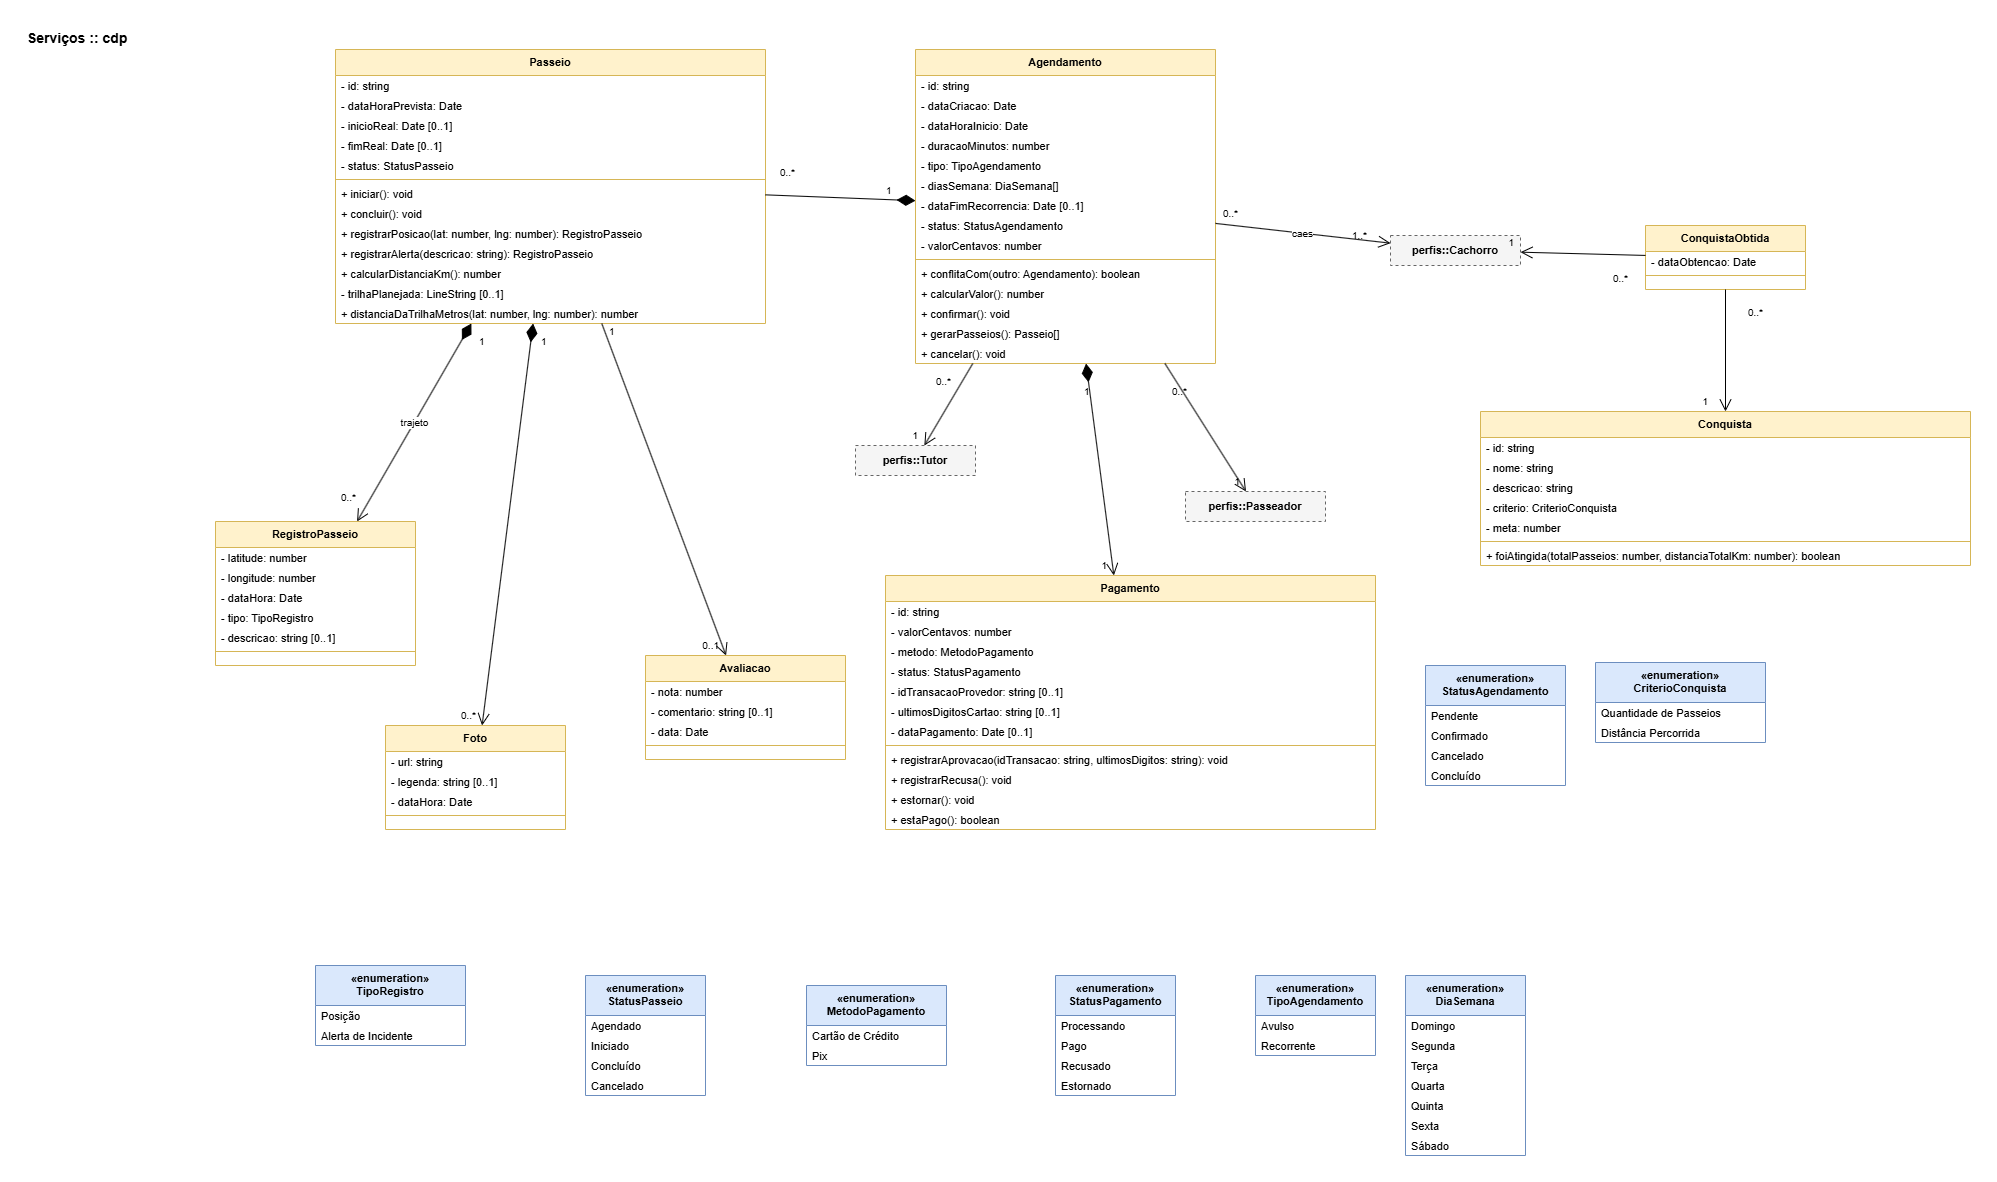
\includegraphics[width=1\textwidth,height=0.85\textheight,keepaspectratio]{figuras/ln-servicos-cdp.png}
	\caption{Projeto da Componente de Domínio do Problema (\texttt{cdp}) do subsistema Serviços.}
	\label{figura-servicos-cdp}
\end{figure}

As principais decisões que levaram a este modelo, em relação ao modelo de requisitos, foram:

\begin{itemize}
	\item \textbf{Agendamento e Passeio.} Um Agendamento recorrente gera vários Passeios (um por ocorrência), por isso a associação é de composição, e os Passeios são criados pela operação \texttt{gerarPasseios()}. A cardinalidade do lado do Passeio é 0..*, pois um Agendamento pendente ainda não possui Passeios. O Agendamento passou a guardar \texttt{dataHoraInicio} (que substitui a data e a hora de início separadas), \texttt{duracaoMinutos}, \texttt{dataFimRecorrencia} (para agendamentos fixos) e \texttt{valorCentavos}, o valor calculado no momento do agendamento. Guardar o valor no Agendamento faz com que alterações posteriores de preço do Passeador só valham para novos contratos (CA06.4).

	\item \textbf{Pagamento associado ao Agendamento.} No modelo de requisitos, o Pagamento aparecia associado ao Passeio, mas a RI-4 (um Agendamento só pode ser confirmado se o Pagamento correspondente estiver pago) e o agendamento recorrente, cobrado mensalmente (Figura 12 do documento de requisitos), mostram que o pagamento se refere ao Agendamento. Em atendimento ao RNF-2, o Pagamento não guarda o número do cartão, apenas o identificador da transação no provedor (\texttt{idTransacaoProvedor}) e os últimos dígitos (\texttt{ultimosDigitosCartao}). A enumeração \texttt{StatusPagamento} tem os valores Processando, Pago, Recusado (CA14.2 a CA14.4) e Estornado, que permite desfazer um pagamento quando o Agendamento é cancelado.

	\item \textbf{Estado do Passeio.} A enumeração \texttt{StatusPasseio} foi redefinida como Agendado, Iniciado, Concluído e Cancelado, que são os estados citados nos critérios de aceitação (CA10.1, CA11.1, CA11.2), em lugar de Realizado e Em\_Andamento. O Passeio passou a ter \texttt{dataHoraPrevista}, \texttt{inicioReal} e \texttt{fimReal} e as operações \texttt{iniciar()}, \texttt{concluir()} e \texttt{calcularDistanciaKm()}.

	\item \textbf{Trilha planejada e desvio de rota.} O modelo de requisitos cita uma ``trilha pré-definida'' (CA10.3), mas não possui user story para cadastrar trilhas. Por isso, a trilha não foi modelada como classe: ela é um dado opcional do Passeio, o atributo \texttt{trilhaPlanejada}, que guarda a linha (sequência de coordenadas) informada ao agendar ou ao iniciar o passeio. A operação \texttt{distanciaDaTrilhaMetros()} calcula a distância de uma posição à trilha, e a classe \texttt{AplExecucaoPasseio} usa esse valor, a cada posição registrada por \texttt{registrarPosicao()}, para detectar o desvio de mais de 100 metros e avisar o tutor por meio de \texttt{NotificadorTempoReal}, o que faz o trajeto aparecer em vermelho. Quando o Passeio não tem trilha planejada, essa verificação não se aplica.

	\item \textbf{Registro do trajeto e alertas.} Como o alerta de incidente do Passeador (minimundo) e o trajeto de GPS são ambos registros ocorridos durante o Passeio, a classe RegistroPasseio recebeu o atributo \texttt{tipo} (Posição ou Alerta de Incidente) e o atributo opcional \texttt{descricao}.

	\item \textbf{Fotos e mural.} A classe Foto é composta pelo Passeio. O mural de um cão (US13) é obtido pelos Passeios dos Agendamentos que o incluem, o que dispensa a associação direta entre Cachorro e Foto do modelo de requisitos.

	\item \textbf{Conquistas.} A classe Conquista do modelo de requisitos foi dividida em duas: \texttt{Conquista}, que define o marco (\texttt{criterio} e \texttt{meta}, por exemplo, 50 km percorridos) e a operação \texttt{foiAtingida()}, e \texttt{ConquistaObtida}, que registra a data em que um Cachorro obteve uma Conquista. Assim, a definição da conquista não é repetida para cada cão.

	\item \textbf{Comentário da Avaliação.} O atributo \texttt{comentario} de Avaliação é opcional (0..1), enquanto a \texttt{nota} é obrigatória (de 1 a 5). O documento de requisitos é inconsistente nesse ponto: o CA15.2 exige nota e comentário, mas a tela de avaliação (Figura 24) marca o comentário como opcional. Prevaleceu a tela, para não impedir que o Tutor avalie um passeio apenas com a nota; a descrição do CA15.2 deve ser ajustada no documento de requisitos para refletir essa decisão.

	\item \textbf{Alertas durante o passeio.} A perda de sinal de GPS por mais de 2 minutos (CA10.4) e o atraso de mais de 15 minutos no encerramento (CA11.3 e CA11.4) não exigiram novas classes nem atributos, pois podem ser calculados a partir de dados já persistidos. A perda de sinal é a diferença entre a hora atual e a \texttt{dataHora} do último \texttt{RegistroPasseio} de um Passeio iniciado. O atraso é a hora atual ultrapassar em mais de 15 minutos a soma de \texttt{dataHoraPrevista} do Passeio com a \texttt{duracaoMinutos} do Agendamento. Uma tarefa periódica do servidor (por exemplo, uma rota acionada por um agendador do ambiente de hospedagem) consulta os Passeios com status ``Iniciado'', aplica essas duas regras e avisa o Tutor por meio de \texttt{NotificadorTempoReal}, o mesmo usado por \texttt{AplExecucaoPasseio}. O cronômetro em vermelho da tela do Passeador (CA11.3) é um comportamento da Camada de Apresentação, que compara a hora atual com o horário previsto de término. Esses alertas são eventos transitórios, não persistidos.

	\item \textbf{Enumerações.} \texttt{TipoAgendamento} (Avulso, Recorrente), \texttt{StatusAgendamento} (Pendente, Confirmado, Cancelado, Concluído), \texttt{DiaSemana}, \texttt{MetodoPagamento} (Cartão de Crédito, Pix), \texttt{CriterioConquista} e \texttt{TipoRegistro}.
\end{itemize}

A Figura~\ref{figura-servicos-cgt} mostra o projeto da Componente de Gerência de Tarefas do subsistema Serviços, e as classes de aplicação são:

\begin{figure}[h]
	\centering
	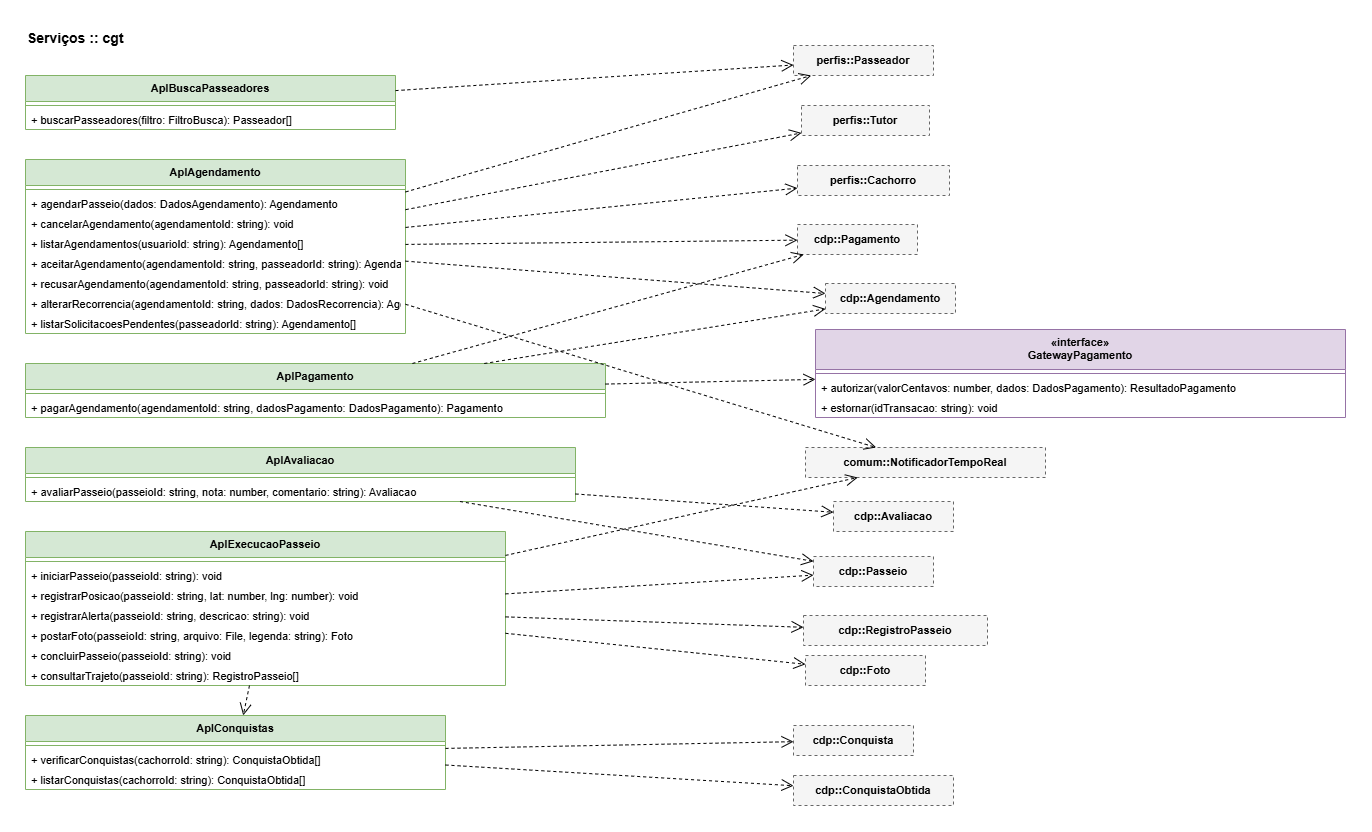
\includegraphics[width=1\textwidth,height=0.85\textheight,keepaspectratio]{figuras/ln-servicos-cgt.png}
	\caption{Projeto da Componente de Gerência de Tarefas (\texttt{cgt}) do subsistema Serviços.}
	\label{figura-servicos-cgt}
\end{figure}

\begin{itemize}
	\item \texttt{AplBuscaPasseadores}: busca de passeadores por filtros (US07);
	\item \texttt{AplAgendamento}: criação de agendamentos avulsos e recorrentes, cancelamento e listagem (US08, US09), além de aceite e recusa pelo Passeador, alteração de recorrência e listagem das solicitações pendentes (CA08.4, CA09.4, CA09.5). Verifica as restrições RI-1, RI-5 e RI-6 e notifica o Tutor por meio de \texttt{NotificadorTempoReal};
	\item \texttt{AplPagamento}: pagamento de um Agendamento (US14), por meio da interface \texttt{GatewayPagamento}, que isola o provedor de pagamento externo;
	\item \texttt{AplExecucaoPasseio}: início, registro de posições e alertas, postagem de fotos, consulta do trajeto e conclusão do Passeio (US10 a US12), publicando os eventos em tempo real por meio de \texttt{NotificadorTempoReal} e acionando \texttt{AplConquistas} na conclusão. Garante que o início real do Passeio não anteceda a data do Agendamento (RI-2) e que o fim real não anteceda o início real (RI-3);
	\item \texttt{AplAvaliacao}: avaliação do Passeio concluído pelo Tutor (US15);
	\item \texttt{AplConquistas}: verificação e listagem das conquistas de um Cachorro (US13).
\end{itemize}

A Figura~\ref{figura-servicos-seq-agendar} detalha o fluxo da operação \texttt{agendarPasseio}. A página de agendamento chama \texttt{AplAgendamento.agendarPasseio()}, que busca o Tutor, o Passeador e os Cachorros nos repositórios e verifica se o Passeador está validado e visível nas buscas. Em seguida, cria o Agendamento, cujo construtor recusa um início anterior à data de criação (RI-1), busca os agendamentos ativos do Passeador e do Cachorro no horário, verifica a existência de conflito para cada um deles (RI-5) e confere se a soma de cães respeita o \texttt{limiteCaes} do Passeador (RI-6). Por fim, calcula o valor, cria o Pagamento associado, salva o Agendamento e exibe a tela de pagamento.

\begin{figure}[h]
	\centering
	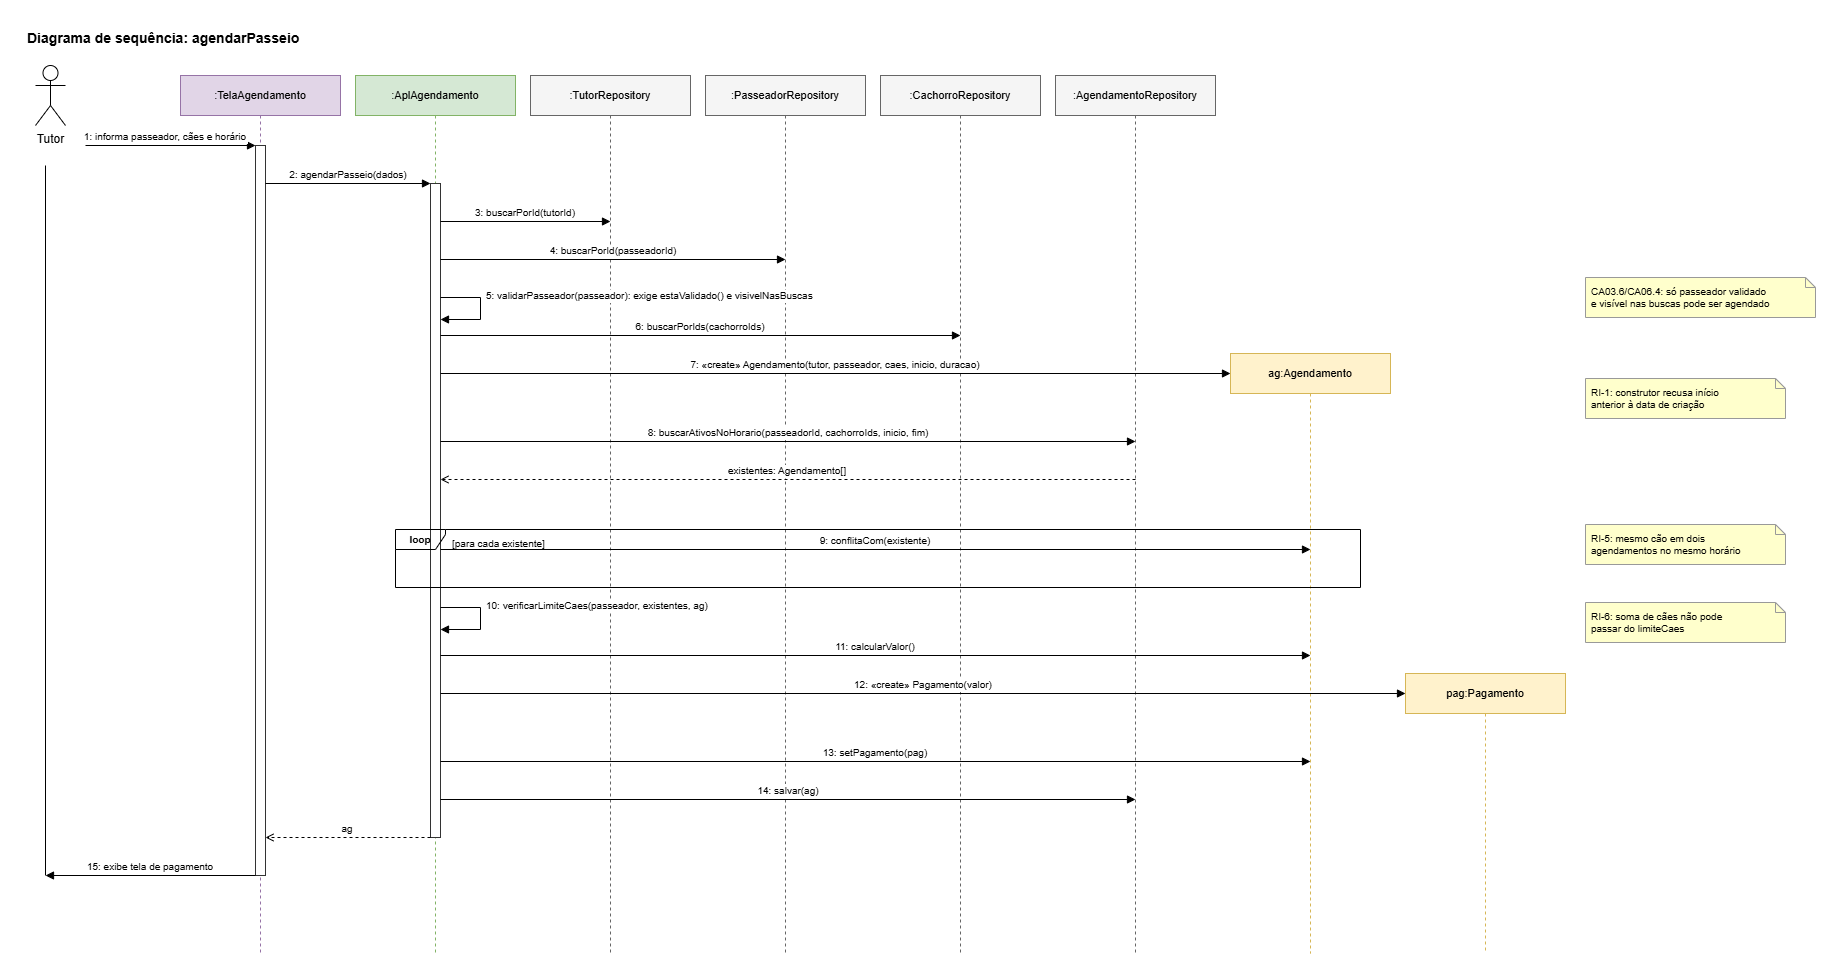
\includegraphics[width=1\textwidth,height=0.85\textheight,keepaspectratio]{figuras/ln-servicos-seq-agendar.png}
	\caption{Diagrama de sequência da operação \texttt{agendarPasseio}.}
	\label{figura-servicos-seq-agendar}
\end{figure}

O pagamento é solicitado logo após a criação do Agendamento. O Agendamento nasce com status ``Pendente'' e o Pagamento com status ``Processando''. Quando o Pagamento é confirmado (``Pago'') e o Passeador aceita a solicitação, o Agendamento passa a ``Confirmado'' (RI-4, CA08.4 e CA09.4). Se o Passeador recusa a solicitação ou o Tutor cancela o Agendamento, o Pagamento é estornado (``Estornado''). Essa escolha prevalece sobre a frase do minimundo que prevê o pagamento após o trajeto, por ser compatível com a RI-4 e com o CA14.5, que impede o início de um Passeio sem pagamento confirmado.


\subsection{Camada de Apresentação}
\label{sec-componentes-servicos-apresentacao}

Esta camada tem as telas de busca de passeadores, de agendamento (avulso e fixo), de acompanhamento do trajeto pelo GPS, de postagem de fotos, de pagamento e de avaliação do passeio, conforme as telas mostradas nas Figuras 7 a 24 do documento de requisitos.


\subsection{Camada de Acesso a Dados}
\label{sec-componentes-servicos-dados}

\begin{sloppypar}
Esta camada guarda e busca os dados do subsistema no banco, usando o Drizzle ORM. Ela é formada pelos repositórios: \texttt{AgendamentoRepository}, \texttt{PasseioRepository}, \texttt{RegistroPasseioRepository}, \texttt{PagamentoRepository}, \texttt{AvaliacaoRepository}, \texttt{FotoRepository}, \texttt{ConquistaRepository} e \texttt{ConquistaObtidaRepository}, que seguem as classes do \texttt{cdp} apresentado na Figura~\ref{figura-servicos-cdp}.
\end{sloppypar}



%=======================================================================================================
\section{Subsistema Suporte}
\label{sec-componentes-suporte}

O subsistema Suporte cuida dos chamados abertos por Tutores ou Passeadores e do atendimento feito pelos Atendentes (US16 e US17).


\subsection{Camada de Negócio}
\label{sec-componentes-suporte-negocio}

A Figura~\ref{figura-suporte-cdp} mostra o projeto da Componente de Domínio do Problema do subsistema Suporte, obtido a partir do diagrama de classes do Documento de Especificação de Requisitos (Figura 37).

\begin{figure}[h]
	\centering
	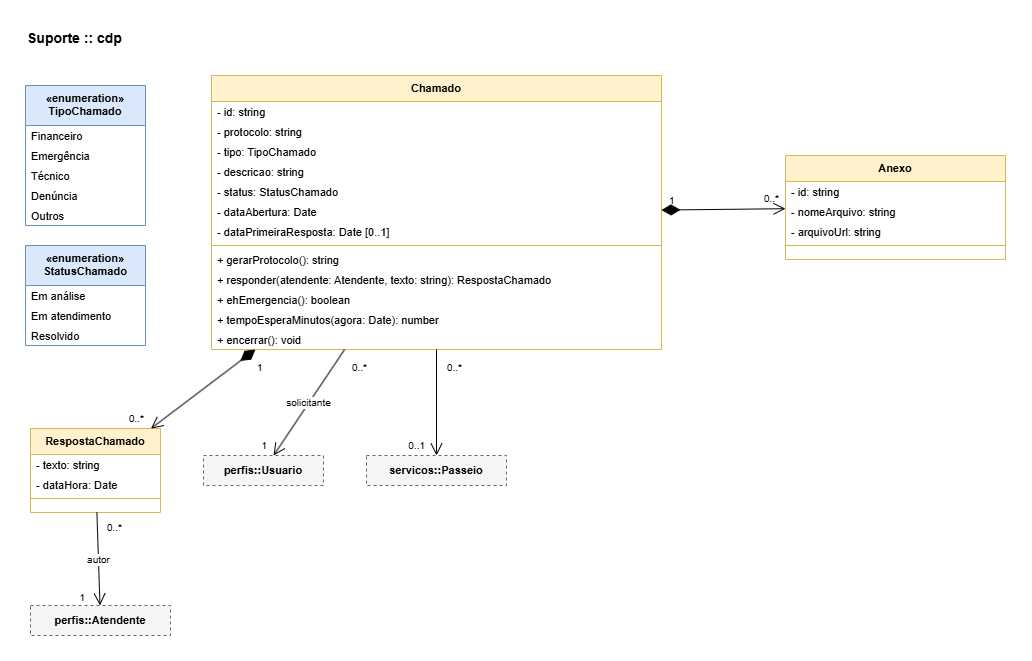
\includegraphics[width=1\textwidth,height=0.8\textheight,keepaspectratio]{figuras/ln-suporte-cdp.png}
	\caption{Projeto da Componente de Domínio do Problema (\texttt{cdp}) do subsistema Suporte.}
	\label{figura-suporte-cdp}
\end{figure}

As principais decisões que levaram a este modelo, em relação ao modelo de requisitos, foram:

\begin{itemize}
	\item \textbf{Solicitante do Chamado.} As duas associações ``abre'', de Tutor e de Passeador, foram substituídas por uma única associação \texttt{solicitante} com a classe Usuário, de Gestão de Perfis.
	\item \textbf{Criação da classe RespostaChamado.} O CA17.5 exige o registro do horário de cada interação do Atendente, e o CA17.4 exige a mudança de status na primeira resposta. Foi criada a classe \texttt{RespostaChamado} (texto e data/hora), composta pelo Chamado e com o Atendente como autor, que substitui a associação ``atende''. O atributo \texttt{dataPrimeiraResposta} em Chamado permite calcular o tempo de primeiro atendimento do RNF-4.
	\item \textbf{Criação da classe Anexo.} O CA17.3 exige que o Atendente visualize ou baixe as fotos e capturas de tela anexadas pelo usuário, o que o modelo de requisitos não representava. Foi criada a classe \texttt{Anexo}, composta pelo Chamado.
	\item \textbf{Chamado e Passeio.} Um Chamado pode se referir opcionalmente a um Passeio (por exemplo, um passeador que não apareceu). Essa associação cria a dependência de Suporte em relação a Serviços mostrada na Figura~\ref{figura-pacotes}.
	\item \textbf{Atributos do Chamado.} O \texttt{protocolo} passou a ser uma \textit{string}, já que os protocolos exibidos nas telas têm letras (por exemplo, EMG-2024-002), e \texttt{dataAbertura} substitui \texttt{data}. As operações \texttt{ehEmergencia()} e \texttt{tempoEsperaMinutos()} apoiam a priorização e o tempo de espera exibidos ao Atendente (CA17.1 e CA17.2).
	\item \textbf{Enumerações.} \texttt{TipoChamado} (Financeiro, Emergência, Técnico, Denúncia, Outros), conforme o CA16.1, e \texttt{StatusChamado} (Em análise, Em atendimento, Resolvido).
\end{itemize}

A Figura~\ref{figura-suporte-cgt} mostra o projeto da Componente de Gerência de Tarefas do subsistema Suporte, e as classes de aplicação são:

\begin{figure}[h]
	\centering
	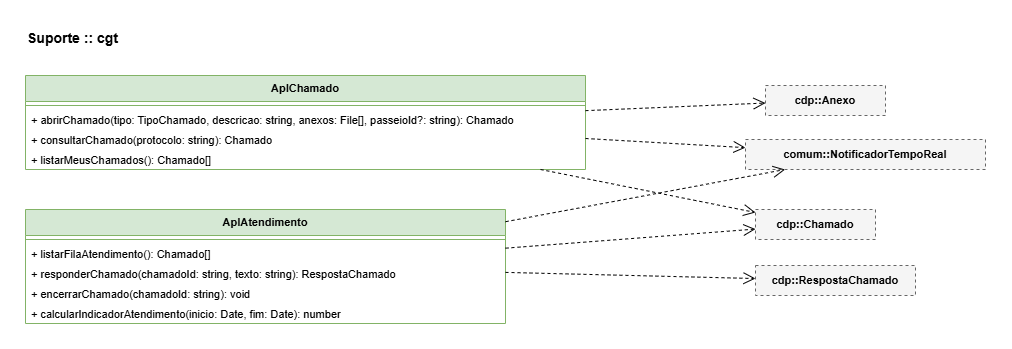
\includegraphics[width=1\textwidth,height=0.7\textheight,keepaspectratio]{figuras/ln-suporte-cgt.png}
	\caption{Projeto da Componente de Gerência de Tarefas (\texttt{cgt}) do subsistema Suporte.}
	\label{figura-suporte-cgt}
\end{figure}

\begin{itemize}
	\item \texttt{AplChamado}: abertura de chamado com tipo, descrição e anexos, consulta por protocolo e listagem dos chamados do usuário (US16). Exige o tipo e a descrição do problema (CA16.1), gera o protocolo e define o status inicial como ``Em análise'' (CA16.2);
	\item \texttt{AplAtendimento}: listagem da fila de atendimento com os chamados de emergência no topo, resposta e encerramento de chamados (US17), e cálculo do indicador de tempo de primeiro atendimento (RNF-4). Ao responder, muda o status para ``Em atendimento'' e notifica o usuário por meio de \texttt{NotificadorTempoReal} (CA16.3).
\end{itemize}


\subsection{Camada de Apresentação}
\label{sec-componentes-suporte-apresentacao}

Esta camada tem a tela de abertura de chamado, usada por Tutores e Passeadores, e as telas da central de atendimento, usadas pelo Atendente, conforme as telas mostradas nas Figuras 25 a 30 do documento de requisitos.


\subsection{Camada de Acesso a Dados}
\label{sec-componentes-suporte-dados}

Esta camada guarda e busca os dados do subsistema no banco, usando o Drizzle ORM. Ela é formada pelos repositórios \texttt{ChamadoRepository}, \texttt{RespostaChamadoRepository} e \texttt{AnexoRepository}, que seguem as classes do \texttt{cdp} apresentado na Figura~\ref{figura-suporte-cdp}.
%\vspace*{1.3cm}

\chapter{Projeto da Lógica de Negócio}
\label{sec-logica-negocio}
\vspace{-1cm}

Este capítulo apresenta o projeto da camada de Negócio dos três subsistemas do Happy Paws: Gestão de Perfis, Serviços e Suporte (Figura~\ref{figura-arquitetura}).

Para organizar a lógica de negócio foi usado o padrão Camada de Serviço (\textit{Service Layer})~\cite{fowler:book02}. Com ele, a camada de Negócio de cada subsistema é dividida em dois componentes:

\begin{itemize}
	\item \textbf{Componente de Domínio do Problema (CDP):} tem as classes do domínio (Tutor, Cachorro, Agendamento, Passeio, Chamado etc.), com seus atributos e os métodos que tratam das regras de cada objeto, como verificar se um Passeio pode ser iniciado ou se um Pagamento já foi pago;
	\item \textbf{Componente de Gerência de Tarefas (CGT):} tem as classes de aplicação (prefixo \texttt{Apl}), que realizam as histórias de usuário. Elas recebem as requisições da camada de Apresentação, buscam os objetos nos repositórios da camada de Acesso a Dados, chamam os métodos do CDP e salvam o resultado. No Happy Paws, cada classe de aplicação é implementada como um módulo de \emph{Server Actions} do Next.js.
\end{itemize}

Esse padrão foi escolhido por três motivos: Primeiro, as \emph{Server Actions} já funcionam como pontos de entrada para cada funcionalidade, o que corresponde diretamente às operações do CGT. Segundo, várias histórias envolvem muitas classes ao mesmo tempo, inclusive de subsistemas diferentes: agendar um passeio, por exemplo, envolve Tutor, Cachorro, Passeador, Agendamento e Pagamento, e essa coordenação fica mais clara em uma classe de aplicação do que espalhada pelas classes de domínio. Terceiro, a relação direta entre classes de aplicação e histórias de usuário facilita a manutenção: quando uma história muda, sabe-se qual classe alterar. Para não cair em um modelo de domínio anêmico, as regras que dizem respeito a um único objeto continuam como métodos das classes do CDP, e o CGT apenas coordena esses objetos.

A Tabela~\ref{tabela-componentes-negocio} resume os componentes da camada de Negócio de cada subsistema.

\begin{footnotesize}
\begin{longtable}{|p{2.6cm}|p{5.4cm}|p{5.4cm}|}
	\caption{Componentes da camada de Negócio por subsistema.}
	\label{tabela-componentes-negocio}\\\hline

	\rowcolor{lightgray}
	\textbf{Subsistema} & \textbf{CDP} & \textbf{CGT} \\\hline
	\endfirsthead
	\hline
	\rowcolor{lightgray}
	\textbf{Subsistema} & \textbf{CDP} & \textbf{CGT} \\\hline
	\endhead

	Gestão de Perfis & \texttt{Usuario}, \texttt{Tutor}, \texttt{Passeador}, \texttt{Atendente}, \texttt{Endereco}, \texttt{Cachorro}, \texttt{ConviteCompartilhamento}, \texttt{Validacao}, \texttt{Documento} & \texttt{AplCadastroUsuario}, \texttt{AplCadastroCachorro}, \texttt{AplCompartilhamentoPerfil}, \texttt{AplValidacaoPasseador} \\\hline

	Serviços & \texttt{Agendamento}, \texttt{Passeio}, \texttt{RegistroPasseio}, \texttt{Foto}, \texttt{Pagamento}, \texttt{Avaliacao}, \texttt{Conquista}, \texttt{ConquistaObtida} & \texttt{AplBuscaPasseadores}, \texttt{AplAgendamento}, \texttt{AplPagamento}, \texttt{AplExecucaoPasseio}, \texttt{AplAvaliacao}, \texttt{AplConquistas} \\\hline

	Suporte & \texttt{Chamado}, \texttt{RespostaChamado} & \texttt{AplChamado}, \texttt{AplAtendimento} \\\hline
\end{longtable}
\end{footnotesize}



\section{Dependências entre os Subsistemas}
\label{sec-logica-dependencias}

Os subsistemas não são independentes: classes de um subsistema fazem referência a classes de outro. A Figura~\ref{figura-ln-pacotes} mostra o diagrama de pacotes da camada de Negócio com essas dependências.

\begin{figure}[h!]
	\centering
	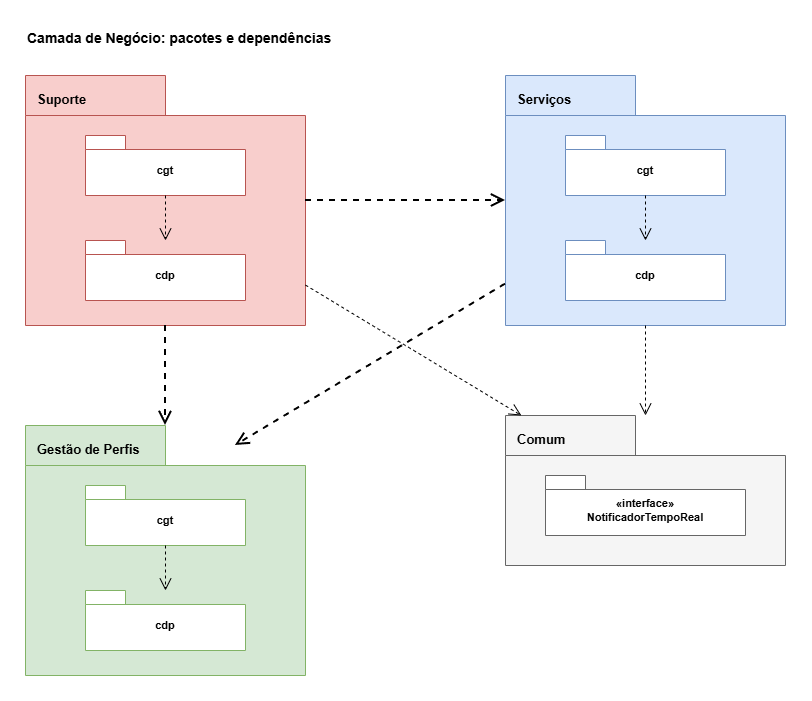
\includegraphics[width=0.85\textwidth]{figuras/ln-pacotes.png}
	\caption{Diagrama de pacotes da camada de Negócio, com as dependências entre os subsistemas.}
	\label{figura-ln-pacotes}
\end{figure}

\begin{itemize}
	\item \textbf{Serviços depende de Gestão de Perfis:} um \texttt{Agendamento} referencia o \texttt{Tutor} que o solicitou, o \texttt{Passeador} que vai realizá-lo e os \texttt{Cachorro}s que vão passear; uma \texttt{ConquistaObtida} referencia o \texttt{Cachorro} que a recebeu. A busca de passeadores também usa o \texttt{Endereco} e as especialidades do \texttt{Passeador};
	\item \textbf{Suporte depende de Gestão de Perfis:} um \texttt{Chamado} é aberto por um \texttt{Usuario} (Tutor ou Passeador) e cada \texttt{RespostaChamado} é escrita por um \texttt{Atendente};
	\item \textbf{Suporte depende de Serviços:} um \texttt{Chamado} pode estar ligado a um \texttt{Passeio}, quando o problema relatado aconteceu durante um passeio (por exemplo, um chamado de emergência).
\end{itemize}

As dependências seguem sempre o mesmo sentido (Suporte $\rightarrow$ Serviços $\rightarrow$ Gestão de Perfis) e não há ciclos. Gestão de Perfis não depende de nenhum outro subsistema e, por isso, pode ser implementado e testado primeiro. As associações entre classes de subsistemas diferentes são navegáveis apenas nesse sentido: um \texttt{Agendamento} conhece o seu \texttt{Tutor}, mas a classe \texttt{Tutor} não guarda a lista de agendamentos (essa consulta é feita pelo \texttt{AgendamentoRepository}).



\section{Decisões de Projeto Comuns aos Subsistemas}
\label{sec-logica-decisoes}

Para passar dos diagramas de classes de análise para os diagramas de classes de projeto, foram tomadas as decisões abaixo, que valem para os três subsistemas:

\begin{itemize}
	\item \textbf{Tipos de dados:} os atributos receberam tipos do TypeScript (\texttt{string}, \texttt{number}, \texttt{boolean} e \texttt{Date}). Identificadores são \texttt{string} no formato UUID. Valores em dinheiro são guardados como \texttt{number} inteiro em centavos (por exemplo, \texttt{valorCentavos}), para evitar erros de arredondamento. Atributos opcionais são indicados com multiplicidade \texttt{[0..1]} e implementados como \texttt{tipo | null};

	\item \textbf{Tipos enumerados:} atributos que só podem assumir alguns valores viraram tipos enumerados (Tabela~\ref{tabela-enumerados}). Isso permite que a camada de Apresentação mostre esses valores em listas de seleção, em vez de campos de texto livre, reduzindo erros de digitação e o número de ações do usuário. No banco, eles são mapeados para \texttt{pgEnum} do Drizzle ORM;

	\item \textbf{Navegabilidade:} as associações passaram a ter sentido de navegação, escolhido a partir das consultas mais frequentes. Por exemplo, \texttt{Passeio} navega para os seus \texttt{RegistroPasseio} (para desenhar o trajeto), mas \texttt{RegistroPasseio} não navega de volta. Entre subsistemas, a navegação segue o sentido das dependências da Seção~\ref{sec-logica-dependencias};

	\item \textbf{Visibilidade e métodos:} todos os atributos são privados. Os métodos de acesso (\texttt{get}/\texttt{set}), construtores e destrutores existem, mas não aparecem nos diagramas. Só são mostrados os métodos que não podem ser deduzidos dos atributos, isto é, os que implementam regras de negócio;

	\item \textbf{Ajuste de hierarquia:} Tutor, Passeador e Atendente têm em comum nome, CPF, e-mail, senha e telefone. Foi criada a superclasse abstrata \texttt{Usuario} com esses dados e com o método de autenticação. Isso também permite que um \texttt{Chamado} seja aberto por qualquer usuário;

	\item \textbf{Eliminação de classe associativa:} a associação entre \texttt{Cachorro} e \texttt{Conquista} guarda a data em que a conquista foi obtida. Como o TypeScript não tem um recurso para classes associativas, ela foi substituída pela classe \texttt{ConquistaObtida}, ligada a \texttt{Cachorro} e a \texttt{Conquista};

	\item \textbf{Segurança:} a senha é guardada apenas como \textit{hash} (\texttt{senhaHash}); \texttt{Pagamento} guarda só o identificador da transação no provedor de pagamento e os quatro últimos dígitos do cartão; e toda operação do CGT recebe o usuário autenticado da sessão e verifica se ele tem permissão sobre os objetos envolvidos (por exemplo, só o tutor e o passeador de um passeio podem ver o seu trajeto), conforme o \ref{rnf-seguranca-dados}.
\end{itemize}

\begin{footnotesize}
\begin{longtable}{|p{3.2cm}|p{5.8cm}|p{4.4cm}|}
	\caption{Tipos enumerados da camada de Negócio.}
	\label{tabela-enumerados}\\\hline

	\rowcolor{lightgray}
	\textbf{Tipo Enumerado} & \textbf{Valores} & \textbf{Usado em} \\\hline
	\endfirsthead
	\hline
	\rowcolor{lightgray}
	\textbf{Tipo Enumerado} & \textbf{Valores} & \textbf{Usado em} \\\hline
	\endhead

	\texttt{Porte} & Pequeno, Médio, Grande & \texttt{Cachorro} \\\hline
	\texttt{Especialidade} & Filhotes, Idosos, Grande Porte, Cães Reativos & \texttt{Passeador} \\\hline
	\texttt{TipoDocumento} & RG, CNH, Selfie, CPF & \texttt{Documento} \\\hline
	\texttt{StatusValidacao} & Em Análise, Validado, Reprovado & \texttt{Validacao} \\\hline
	\texttt{StatusConvite} & Pendente, Ativo, Recusado & \texttt{ConviteCompartilhamento} \\\hline
	\texttt{TipoAgendamento} & Avulso, Recorrente & \texttt{Agendamento} \\\hline
	\texttt{DiaSemana} & Domingo a Sábado & \texttt{Agendamento} (passeios fixos) \\\hline
	\texttt{StatusAgendamento} & Pendente, Confirmado, Cancelado, Concluído & \texttt{Agendamento} \\\hline
	\texttt{StatusPasseio} & Agendado, Iniciado, Concluído, Cancelado & \texttt{Passeio} \\\hline
	\texttt{TipoRegistro} & Posição, Alerta de Incidente & \texttt{RegistroPasseio} \\\hline
	\texttt{MetodoPagamento} & Cartão de Crédito, Pix & \texttt{Pagamento} \\\hline
	\texttt{StatusPagamento} & Processando, Pago, Recusado, Estornado & \texttt{Pagamento} \\\hline
	\texttt{CriterioConquista} & Quantidade de Passeios, Distância Percorrida & \texttt{Conquista} \\\hline
	\texttt{TipoChamado} & Financeiro, Emergência, Técnico, Denúncia, Outros & \texttt{Chamado} \\\hline
	\texttt{StatusChamado} & Em análise, Em atendimento, Resolvido & \texttt{Chamado} \\\hline
\end{longtable}
\end{footnotesize}



\section{Subsistema Gestão de Perfis}
\label{sec-logica-perfis}

O subsistema Gestão de Perfis cuida do cadastro de tutores, cães e passeadores, da validação de identidade dos passeadores e do compartilhamento de perfis de cães entre tutores (US01 a US06).


\subsection{Componente de Domínio do Problema}
\label{sec-logica-perfis-cdp}

A Figura~\ref{figura-ln-perfis-cdp} mostra o diagrama de classes do CDP do subsistema Gestão de Perfis.

\begin{figure}[h!]
	\centering
	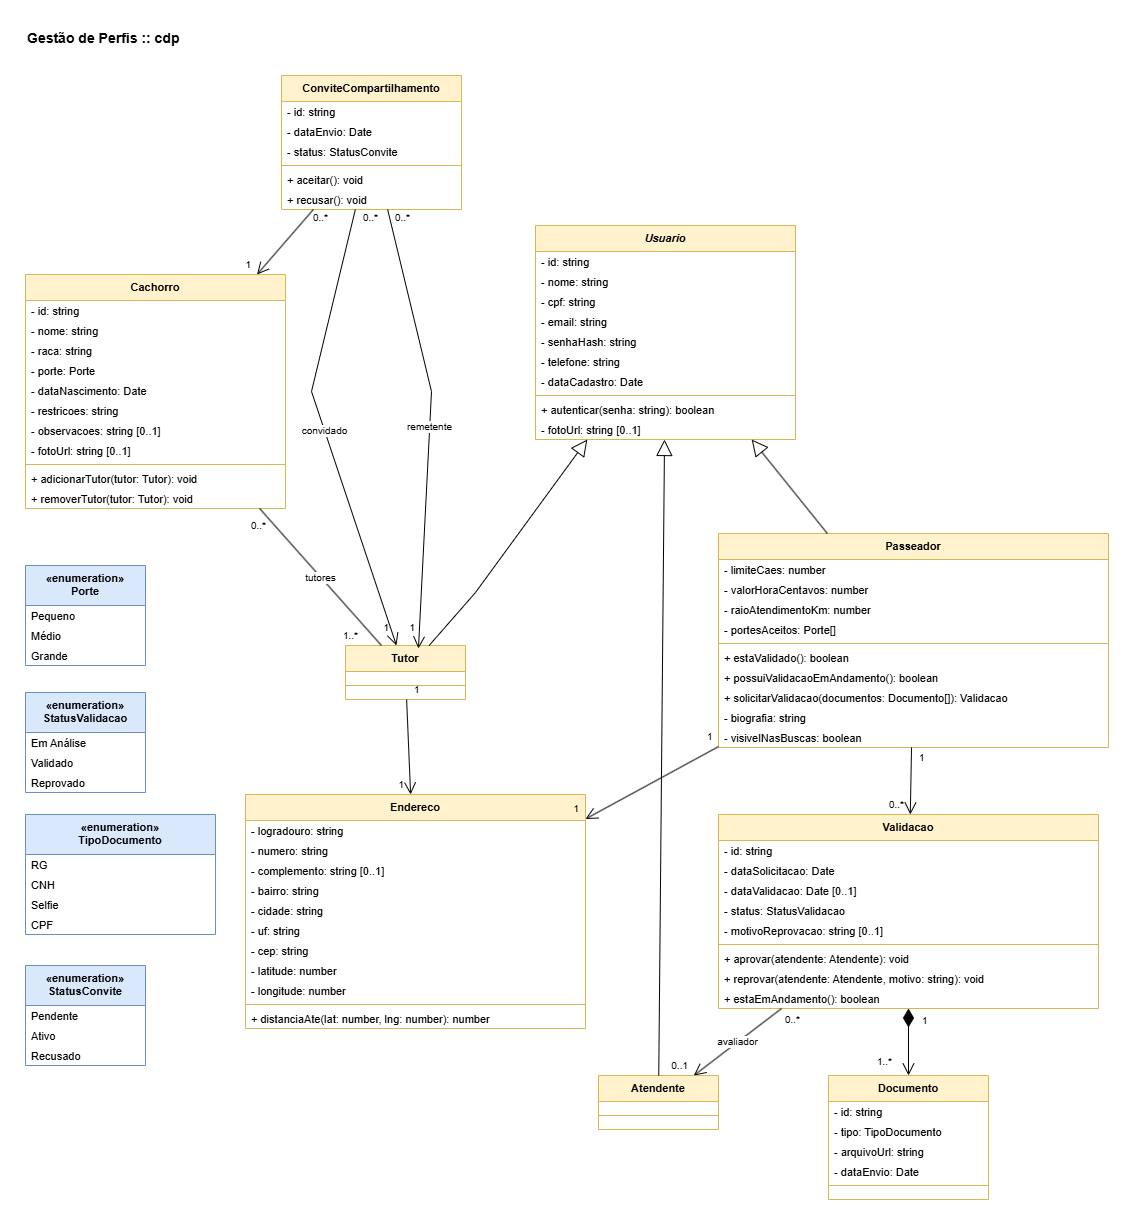
\includegraphics[width=\textwidth]{figuras/ln-perfis-cdp.png}
	\caption{Diagrama de classes do CDP do subsistema Gestão de Perfis.}
	\label{figura-ln-perfis-cdp}
\end{figure}

As principais classes e métodos são:

\begin{itemize}
	\item \texttt{Usuario} (abstrata): superclasse de \texttt{Tutor}, \texttt{Passeador} e \texttt{Atendente}, com \texttt{id}, \texttt{nome}, \texttt{cpf}, \texttt{email}, \texttt{senhaHash}, \texttt{telefone} e \texttt{dataCadastro}. O método \texttt{autenticar(senha)} compara a senha informada com o \textit{hash} guardado;

	\item \texttt{Passeador}: tem \texttt{limiteCaes}, \texttt{valorHoraCentavos}, \texttt{raioAtendimentoKm} e uma lista de \texttt{Especialidade}. O método \texttt{estaValidado()} indica se o passeador já teve uma validação aprovada (só passeadores validados aparecem na busca); \texttt{possuiValidacaoEmAndamento()} e \texttt{solicitarValidacao(documentos)} garantem que o passeador não tenha mais de uma Validação ao mesmo tempo (RI-4);

	\item \texttt{Endereco}: além dos dados do endereço, guarda \texttt{latitude} e \texttt{longitude}. O método \texttt{distanciaAte(lat, lng)} é usado na busca de passeadores por geolocalização;

	\item \texttt{Cachorro}: tem \texttt{nome}, \texttt{raca}, \texttt{porte}, \texttt{dataNascimento}, \texttt{observacoes} e \texttt{fotoUrl}, e uma associação com um ou mais \texttt{Tutor}es, navegável nos dois sentidos, pois as consultas ``cães de um tutor'' e ``tutores de um cão'' são frequentes. O método \texttt{removerTutor(tutor)} impede a remoção do último tutor, garantindo a RI-3;

	\item \texttt{ConviteCompartilhamento}: classe criada para representar o convite da US05. Liga o cão, o tutor que convida e o tutor convidado, e tem os métodos \texttt{aceitar()}, que adiciona o convidado como tutor do cão, e \texttt{recusar()};

	\item \texttt{Validacao} e \texttt{Documento}: uma Validação é composta por um ou mais Documentos enviados pelo passeador. Os métodos \texttt{aprovar(atendente)} e \texttt{reprovar(atendente, motivo)} registram o atendente responsável e a data da validação, conferindo se a data de envio de todos os documentos é anterior ou igual a ela (RI-5).
\end{itemize}

As regras RI-1 e RI-2 (CPF e e-mail únicos) dependem de outros objetos já cadastrados e, por isso, não ficam em uma classe do CDP: elas são verificadas pela classe de aplicação \texttt{AplCadastroUsuario}, que consulta os repositórios antes de salvar.


\subsection{Componente de Gerência de Tarefas}
\label{sec-logica-perfis-cgt}

A Figura~\ref{figura-ln-perfis-cgt} mostra as classes do CGT do subsistema e a Tabela~\ref{tabela-cgt-perfis} descreve suas operações.

\begin{figure}[h!]
	\centering
	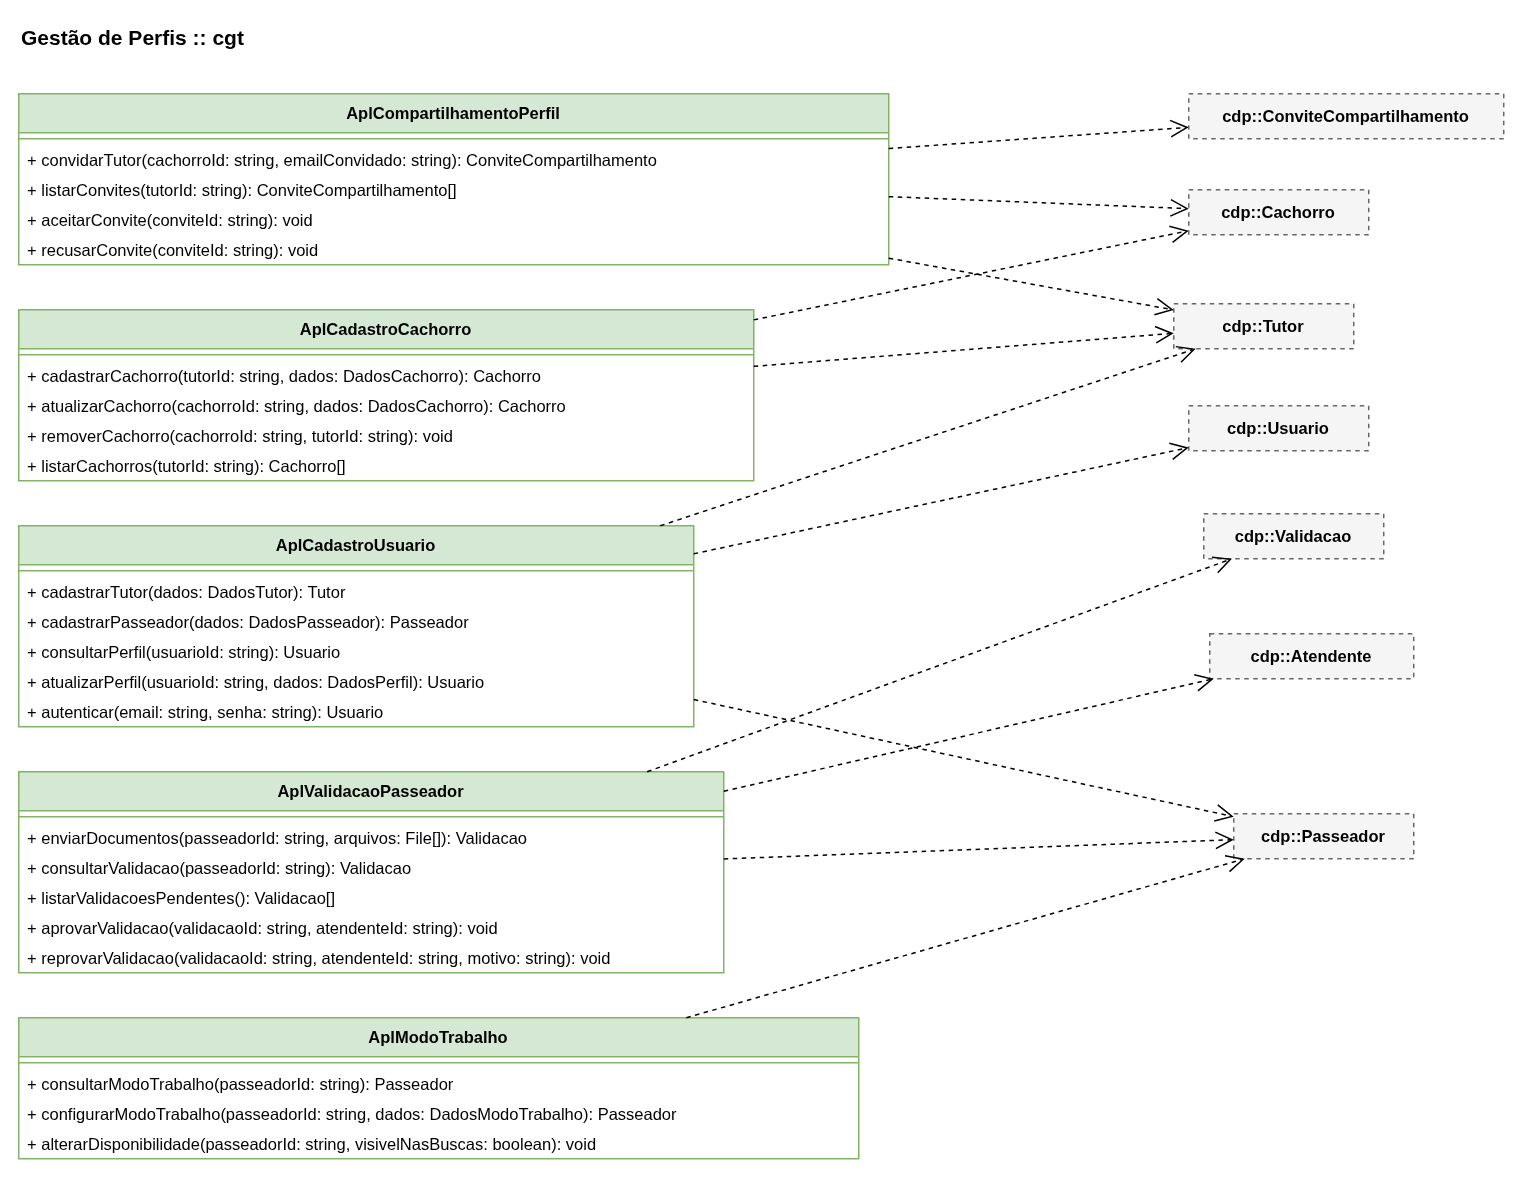
\includegraphics[width=\textwidth]{figuras/ln-perfis-cgt.png}
	\caption{Diagrama de classes do CGT do subsistema Gestão de Perfis.}
	\label{figura-ln-perfis-cgt}
\end{figure}

\begin{footnotesize}
\begin{longtable}{|p{3.4cm}|p{7.6cm}|p{2.4cm}|}
	\caption{Operações do CGT do subsistema Gestão de Perfis.}
	\label{tabela-cgt-perfis}\\\hline

	\rowcolor{lightgray}
	\textbf{Classe} & \textbf{Operações} & \textbf{Regras} \\\hline
	\endfirsthead
	\hline
	\rowcolor{lightgray}
	\textbf{Classe} & \textbf{Operações} & \textbf{Regras} \\\hline
	\endhead

	\texttt{AplCadastroUsuario} & \texttt{cadastrarTutor(dados)}: cadastra um tutor e seu endereço. \newline
	\texttt{cadastrarPasseador(dados)}: cadastra um passeador, com limite de cães e especialidades. \newline
	\texttt{atualizarPerfil(usuarioId, dados)}: altera os dados do perfil. \newline
	\texttt{autenticar(email, senha)}: faz o \textit{login} do usuário. & RI-1, RI-2 \\\hline

	\texttt{AplCadastroCachorro} & \texttt{cadastrarCachorro(tutorId, dados)}: cadastra um cão ligado ao tutor. \newline
	\texttt{atualizarCachorro(cachorroId, dados)}: altera os dados do cão. \newline
	\texttt{removerCachorro(cachorroId, tutorId)}: remove o cão ou desvincula o tutor. \newline
	\texttt{listarCachorros(tutorId)}: lista os cães do tutor. & RI-3 \\\hline

	\texttt{AplCompartilhamentoPerfil} & \texttt{convidarTutor(cachorroId, emailConvidado)}: cria um convite de compartilhamento. \newline
	\texttt{aceitarConvite(conviteId)}: o convidado passa a ser tutor do cão. \newline
	\texttt{recusarConvite(conviteId)}: encerra o convite. & US05 \\\hline

	\texttt{AplValidacaoPasseador} & \texttt{enviarDocumentos(passeadorId, arquivos)}: envia os documentos e abre uma validação. \newline
	\texttt{listarValidacoesPendentes()}: lista as validações para o Atendente. \newline
	\texttt{aprovarValidacao(validacaoId)}: aprova a validação. \newline
	\texttt{reprovarValidacao(validacaoId, motivo)}: reprova a validação, informando o motivo. & RI-4, RI-5 \\\hline
\end{longtable}
\end{footnotesize}



\section{Subsistema Serviços}
\label{sec-logica-servicos}

O subsistema Serviços cuida da busca por passeadores, do agendamento de passeios (avulsos ou fixos), da execução do passeio em tempo real (GPS, alertas e fotos), do pagamento, da avaliação e das conquistas do pet (US07 a US15).


\subsection{Componente de Domínio do Problema}
\label{sec-logica-servicos-cdp}

A Figura~\ref{figura-ln-servicos-cdp} mostra o diagrama de classes do CDP do subsistema Serviços. As classes \texttt{Tutor}, \texttt{Passeador} e \texttt{Cachorro} aparecem no diagrama como classes do pacote de Gestão de Perfis.

\begin{figure}[h!]
	\centering
	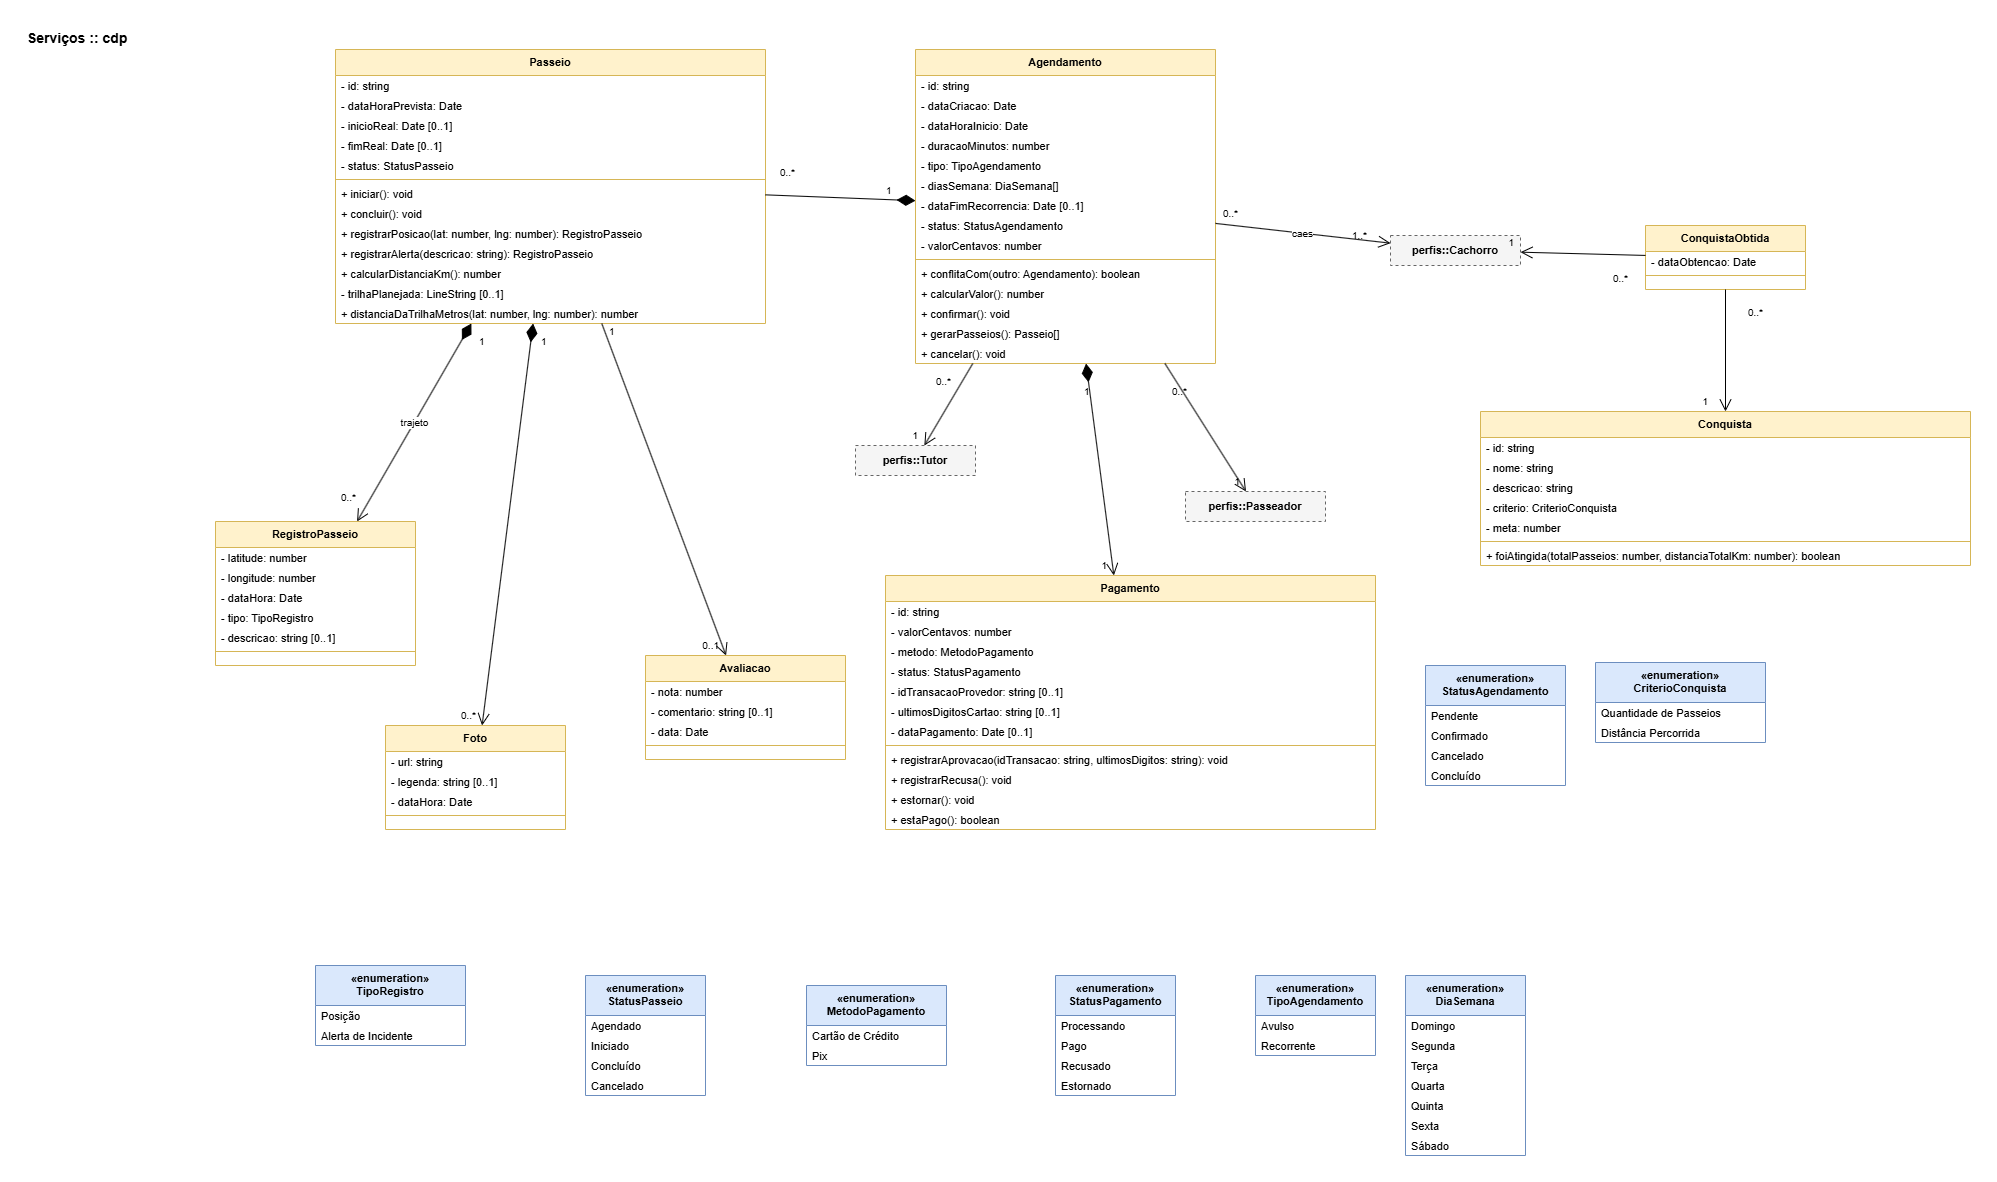
\includegraphics[width=\textwidth]{figuras/ln-servicos-cdp.png}
	\caption{Diagrama de classes do CDP do subsistema Serviços.}
	\label{figura-ln-servicos-cdp}
\end{figure}

As principais classes e métodos são:

\begin{itemize}
	\item \texttt{Agendamento}: tem \texttt{dataCriacao}, \texttt{dataHoraInicio}, \texttt{duracaoMinutos}, \texttt{tipo} (avulso ou fixo), \texttt{diasSemana} e \texttt{dataFimRecorrencia} (só para passeios fixos), \texttt{status} e \texttt{valorCentavos}. Seus métodos são:
	\begin{itemize}
		\item \texttt{conflitaCom(outro)}: indica se dois agendamentos usam o mesmo cão no mesmo horário (RI-5);
		\item \texttt{calcularValor()}: calcula o valor a partir do valor por hora do passeador, da duração e do número de cães;
		\item \texttt{confirmar()}: só muda o status para ``Confirmado'' se o Pagamento estiver ``Pago'' (RI-4);
		\item \texttt{gerarPasseios()}: cria um Passeio para um agendamento avulso, ou um Passeio para cada dia da recorrência de um agendamento fixo;
		\item \texttt{cancelar()}.
	\end{itemize}
	O construtor recusa um \texttt{dataHoraInicio} anterior à \texttt{dataCriacao} (RI-1);

	\item \texttt{Passeio}: tem \texttt{dataHoraPrevista}, \texttt{inicioReal}, \texttt{fimReal} e \texttt{status}. Os métodos \texttt{iniciar()} e \texttt{concluir()} mudam o status e registram o início e o fim reais, conferindo-os com o Agendamento (RI-2 e RI-3). Os métodos \texttt{registrarPosicao(lat, lng)} e \texttt{registrarAlerta(descricao)} só aceitam registros quando o passeio está ``Iniciado''. O método \texttt{calcularDistanciaKm()} soma as distâncias entre as posições do trajeto;

	\item \texttt{RegistroPasseio}: cada ponto do trajeto ou alerta de incidente, com \texttt{latitude}, \texttt{longitude}, \texttt{dataHora}, \texttt{tipo} e \texttt{descricao}. \texttt{Foto} guarda \texttt{url}, \texttt{legenda} e \texttt{dataHora}. As duas classes são partes do Passeio (composição);

	\item \texttt{Pagamento}: tem \texttt{valorCentavos}, \texttt{metodo}, \texttt{status}, \texttt{idTransacaoProvedor}, \texttt{ultimosDigitosCartao} e \texttt{dataPagamento}. Os métodos \texttt{registrarAprovacao(idTransacao, ultimosDigitos)}, \texttt{registrarRecusa()}, \texttt{estornar()} e \texttt{estaPago()} controlam o seu status. O número completo do cartão nunca chega a essa classe;

	\item \texttt{Avaliacao}: \texttt{nota} (de 1 a 5), \texttt{comentario} e \texttt{data}, ligada a um Passeio concluído;

	\item \texttt{Conquista} e \texttt{ConquistaObtida}: \texttt{Conquista} define o critério e a meta (por exemplo, 10 passeios ou 50 km percorridos) e tem o método \texttt{foiAtingida(totalPasseios, distanciaTotalKm)}. \texttt{ConquistaObtida} registra quando um Cachorro recebeu uma Conquista (US13).
\end{itemize}

A regra do limite de cães do passeador (RI-6) depende de todos os agendamentos do passeador naquele horário. Por isso, ela é verificada pela classe de aplicação \texttt{AplAgendamento}, que soma os cães dos agendamentos existentes com os do novo agendamento e compara com o \texttt{limiteCaes} do \texttt{Passeador}.


\subsection{Componente de Gerência de Tarefas}
\label{sec-logica-servicos-cgt}

A Figura~\ref{figura-ln-servicos-cgt} mostra as classes do CGT do subsistema e a Tabela~\ref{tabela-cgt-servicos} descreve suas operações. As classes \texttt{AplPagamento} e \texttt{AplExecucaoPasseio} usam duas interfaces para serviços externos: \texttt{GatewayPagamento}, que envia o pagamento ao provedor externo, e \texttt{NotificadorTempoReal}, que publica as posições e os alertas para o tutor por \textit{Server-Sent Events} (SSE), conforme o RNF-3 (Seção~\ref{rnf-tempo-real}).

\begin{figure}[h!]
	\centering
	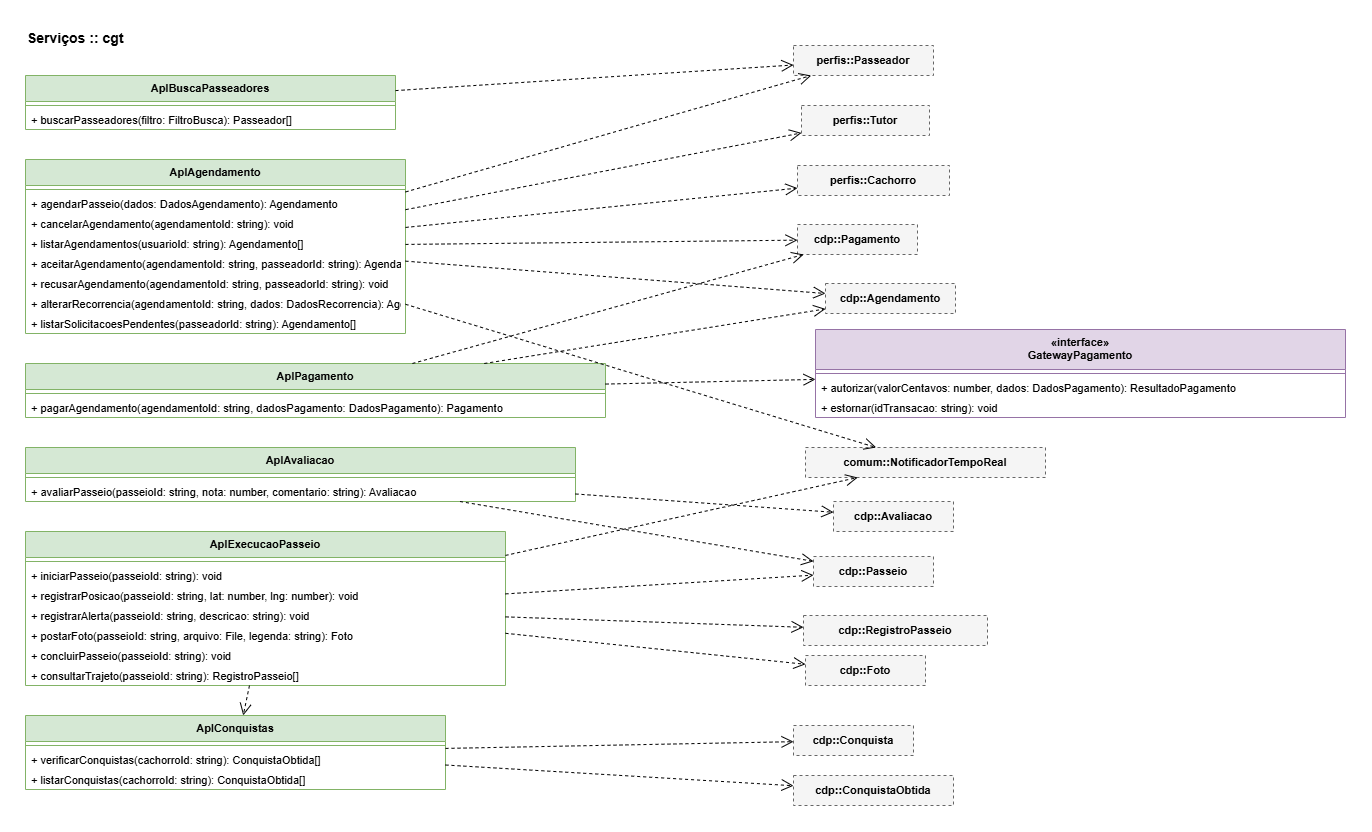
\includegraphics[width=\textwidth]{figuras/ln-servicos-cgt.png}
	\caption{Diagrama de classes do CGT do subsistema Serviços.}
	\label{figura-ln-servicos-cgt}
\end{figure}

\begin{footnotesize}
\begin{longtable}{|p{3.4cm}|p{7.6cm}|p{2.4cm}|}
	\caption{Operações do CGT do subsistema Serviços.}
	\label{tabela-cgt-servicos}\\\hline

	\rowcolor{lightgray}
	\textbf{Classe} & \textbf{Operações} & \textbf{Regras} \\\hline
	\endfirsthead
	\hline
	\rowcolor{lightgray}
	\textbf{Classe} & \textbf{Operações} & \textbf{Regras} \\\hline
	\endhead

	\texttt{AplBuscaPasseadores} & \texttt{buscarPasseadores(filtro)}: retorna os passeadores validados que atendem a localização, a especialidade e o horário informados, ordenados por distância. & --- \\\hline

	\texttt{AplAgendamento} & \texttt{agendarPasseio(dados)}: cria um agendamento avulso ou fixo, com pagamento pendente. \newline
	\texttt{cancelarAgendamento(agendamentoId)}: cancela o agendamento e os passeios futuros. \newline
	\texttt{listarAgendamentos(usuarioId)}: lista os agendamentos do tutor ou do passeador. & RI-1, RI-5, RI-6 \\\hline

	\texttt{AplPagamento} & \texttt{pagarAgendamento(agendamentoId, dadosPagamento)}: envia o pagamento ao provedor externo; se aprovado, confirma o agendamento e gera os passeios. & RI-4 \\\hline

	\texttt{AplExecucaoPasseio} & \texttt{iniciarPasseio(passeioId)}: inicia o passeio. \newline
	\texttt{registrarPosicao(passeioId, lat, lng)}: guarda a posição e a publica para o tutor. \newline
	\texttt{registrarAlerta(passeioId, descricao)}: registra e publica um alerta de incidente. \newline
	\texttt{postarFoto(passeioId, arquivo, legenda)}: guarda uma foto do passeio. \newline
	\texttt{concluirPasseio(passeioId)}: conclui o passeio e chama \texttt{AplConquistas}. \newline
	\texttt{consultarTrajeto(passeioId)}: retorna o trajeto, só para o tutor e o passeador do passeio. & RI-2, RI-3 \\\hline

	\texttt{AplAvaliacao} & \texttt{avaliarPasseio(passeioId, nota, comentario)}: registra a avaliação de um passeio concluído. & --- \\\hline

	\texttt{AplConquistas} & \texttt{verificarConquistas(cachorroId)}: confere o histórico do cão e cria as novas conquistas obtidas. \newline
	\texttt{listarConquistas(cachorroId)}: lista as conquistas do cão. & US13 \\\hline
\end{longtable}
\end{footnotesize}

A Figura~\ref{figura-ln-seq-agendar} mostra o diagrama de sequência da operação \texttt{agendarPasseio}, que é a que envolve mais classes no sistema. A sequência é a seguinte:

\begin{enumerate}
	\item A tela de agendamento chama \texttt{agendarPasseio(dados)} da classe \texttt{AplAgendamento};
	\item \texttt{AplAgendamento} busca o \texttt{Tutor}, o \texttt{Passeador} e os \texttt{Cachorro}s nos repositórios de Gestão de Perfis;
	\item Um novo \texttt{Agendamento} é criado, e o construtor verifica a RI-1;
	\item \texttt{AplAgendamento} busca no \texttt{AgendamentoRepository} os agendamentos pendentes ou confirmados no mesmo horário e, para cada um, chama \texttt{conflitaCom()} do novo agendamento (RI-5);
	\item A soma dos cães desses agendamentos com os do novo agendamento é comparada com o \texttt{limiteCaes} do \texttt{Passeador} (RI-6);
	\item O valor é calculado com \texttt{calcularValor()} e é criado um \texttt{Pagamento} com status ``Pendente'';
	\item O agendamento é salvo e devolvido à tela, que leva o tutor para a tela de pagamento.
\end{enumerate}

\begin{figure}[h!]
	\centering
	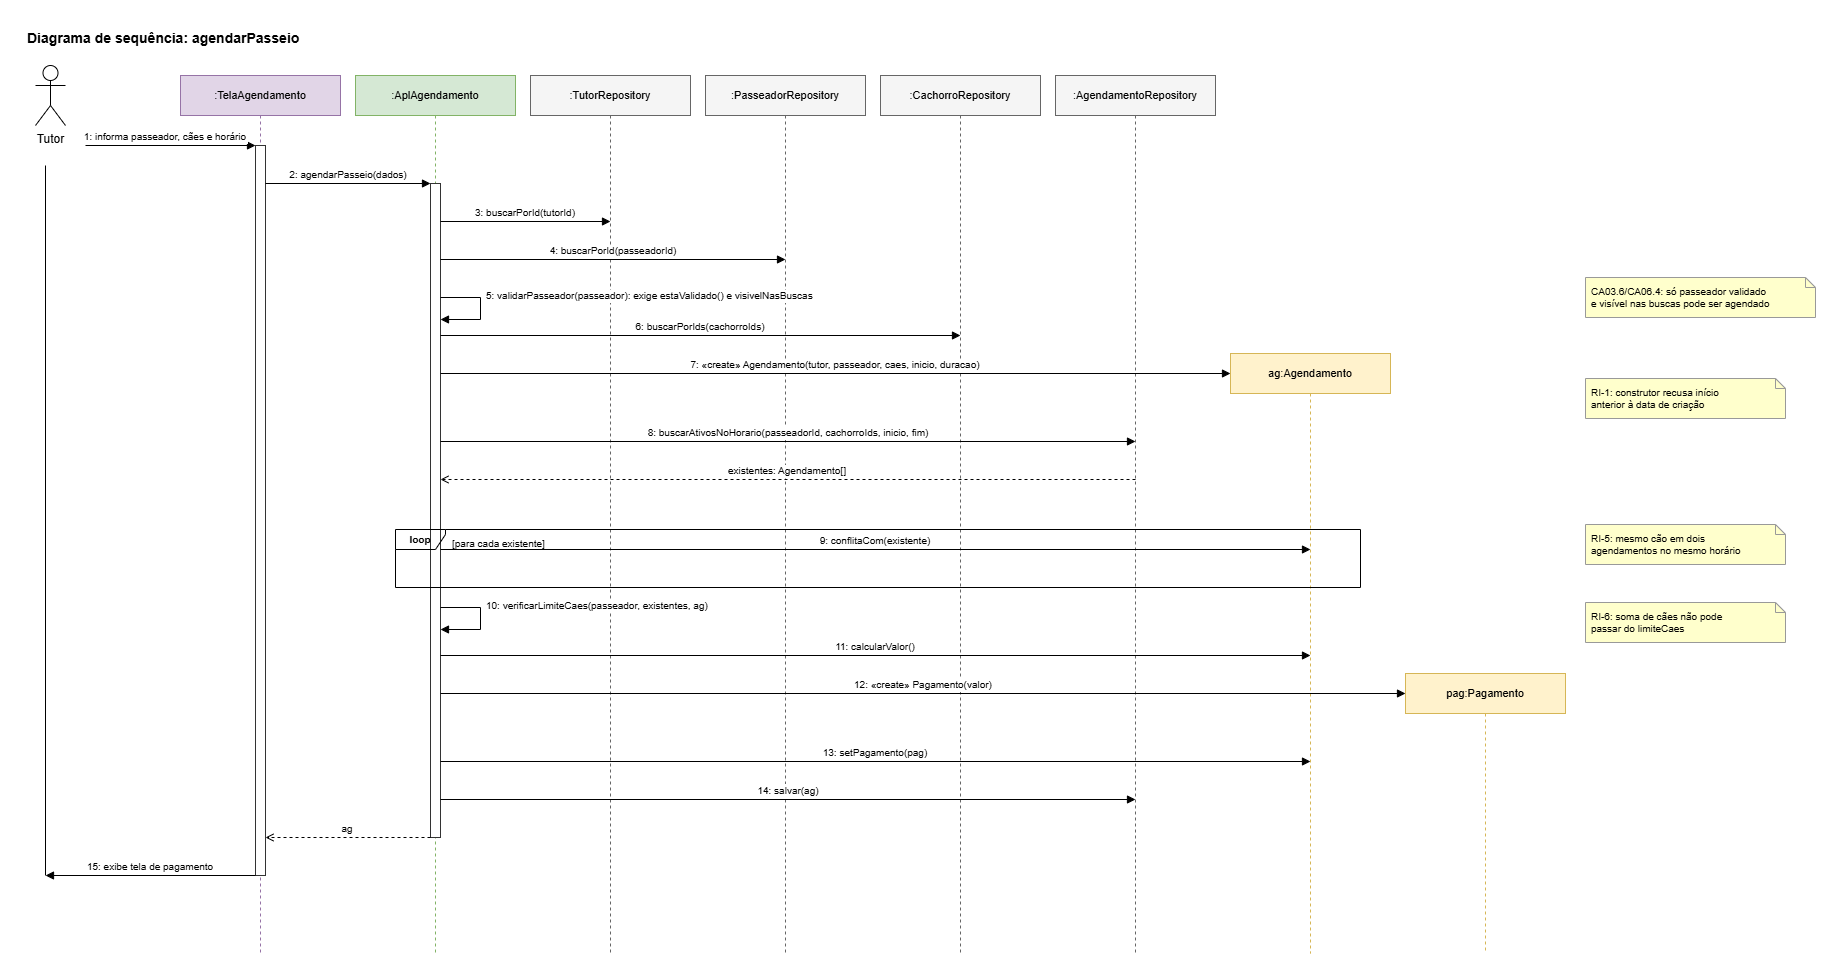
\includegraphics[width=\textwidth]{figuras/ln-servicos-seq-agendar.png}
	\caption{Diagrama de sequência da operação \texttt{agendarPasseio}.}
	\label{figura-ln-seq-agendar}
\end{figure}



\section{Subsistema Suporte}
\label{sec-logica-suporte}

O subsistema Suporte cuida dos chamados abertos por Tutores ou Passeadores e do atendimento feito pelos Atendentes (US16 e US17).


\subsection{Componente de Domínio do Problema}
\label{sec-logica-suporte-cdp}

A Figura~\ref{figura-ln-suporte-cdp} mostra o diagrama de classes do CDP do subsistema Suporte. As classes \texttt{Usuario} e \texttt{Atendente}, de Gestão de Perfis, e \texttt{Passeio}, de Serviços, aparecem no diagrama como classes de outros pacotes.

\begin{figure}[h!]
	\centering
	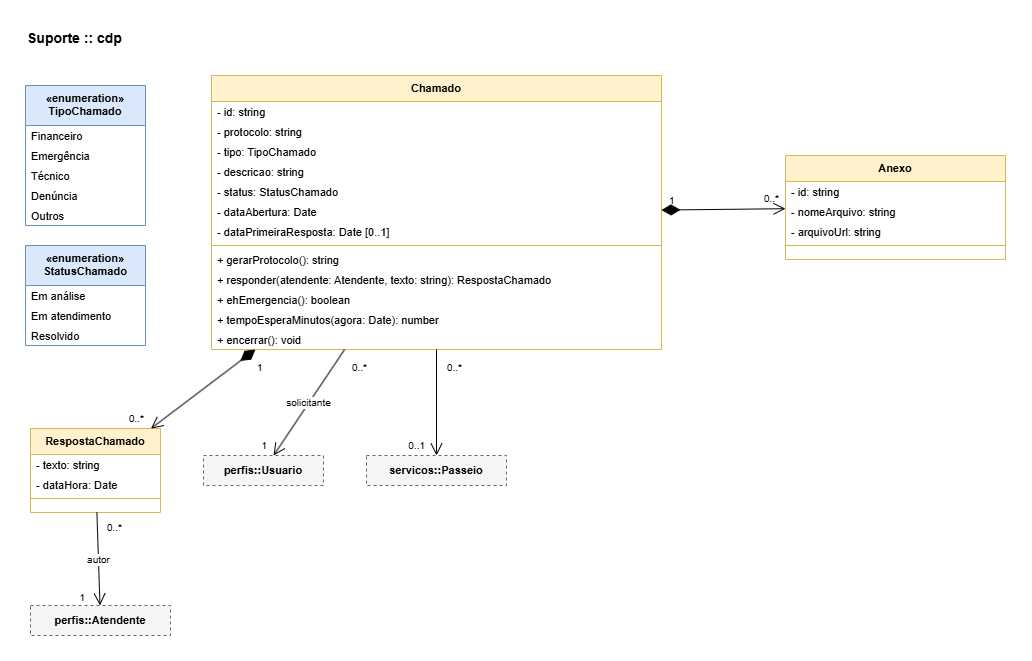
\includegraphics[width=0.85\textwidth]{figuras/ln-suporte-cdp.png}
	\caption{Diagrama de classes do CDP do subsistema Suporte.}
	\label{figura-ln-suporte-cdp}
\end{figure}

As classes deste componente são:

\begin{itemize}
	\item \texttt{Chamado}: tem \texttt{protocolo}, \texttt{tipo}, \texttt{descricao}, \texttt{status}, \texttt{dataAbertura} e \texttt{dataPrimeiraResposta}. Está ligado ao \texttt{Usuario} que o abriu e, opcionalmente, a um \texttt{Passeio}. Seus métodos são:
	\begin{itemize}
		\item \texttt{gerarProtocolo()}: chamado no construtor, que também coloca o status inicial como ``Em análise'' e exige o tipo e a descrição;
		\item \texttt{responder(atendente, texto)}: cria uma \texttt{RespostaChamado}, muda o status para ``Em atendimento'' e, se for a primeira resposta, guarda a \texttt{dataPrimeiraResposta};
		\item \texttt{ehEmergencia()}: indica se o chamado é do tipo ``Emergência'', usado para ordenar a fila de atendimento;
		\item \texttt{tempoEsperaMinutos(agora)}: calcula há quanto tempo o chamado espera a primeira resposta;
		\item \texttt{encerrar()}: muda o status para ``Resolvido''.
	\end{itemize}

	\item \texttt{RespostaChamado}: cada resposta do Atendente, com \texttt{texto} e \texttt{dataHora}, ligada ao \texttt{Atendente} que a escreveu. É parte do Chamado (composição) e guarda o horário de cada resposta para controle interno.
\end{itemize}


\subsection{Componente de Gerência de Tarefas}
\label{sec-logica-suporte-cgt}

A Figura~\ref{figura-ln-suporte-cgt} mostra as classes do CGT do subsistema e a Tabela~\ref{tabela-cgt-suporte} descreve suas operações.

\begin{figure}[h!]
	\centering
	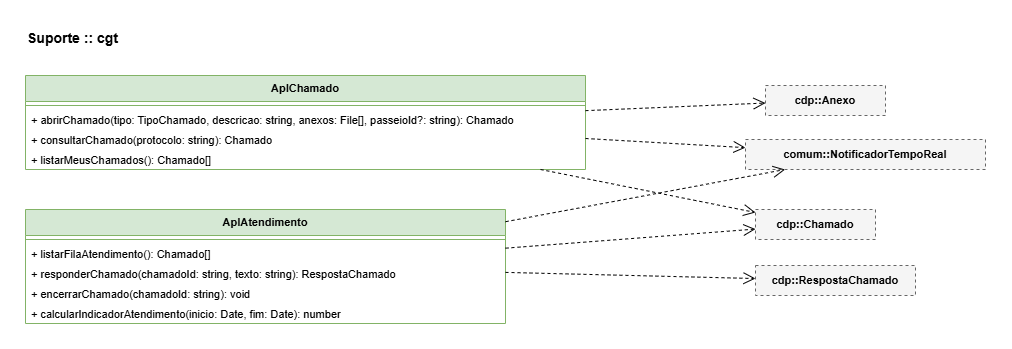
\includegraphics[width=0.85\textwidth]{figuras/ln-suporte-cgt.png}
	\caption{Diagrama de classes do CGT do subsistema Suporte.}
	\label{figura-ln-suporte-cgt}
\end{figure}

\begin{footnotesize}
\begin{longtable}{|p{3.4cm}|p{7.6cm}|p{2.4cm}|}
	\caption{Operações do CGT do subsistema Suporte.}
	\label{tabela-cgt-suporte}\\\hline

	\rowcolor{lightgray}
	\textbf{Classe} & \textbf{Operações} & \textbf{Regras} \\\hline
	\endfirsthead
	\hline
	\rowcolor{lightgray}
	\textbf{Classe} & \textbf{Operações} & \textbf{Regras} \\\hline
	\endhead

	\texttt{AplChamado} & \texttt{abrirChamado(tipo, descricao, passeioId)}: abre um chamado para o usuário autenticado; se for do tipo ``Emergência'', avisa os atendentes pelo \texttt{NotificadorTempoReal}. \newline
	\texttt{consultarChamado(protocolo)}: mostra o chamado e suas respostas. \newline
	\texttt{listarMeusChamados()}: lista os chamados do usuário. & US16 \\\hline

	\texttt{AplAtendimento} & \texttt{listarFilaAtendimento()}: lista os chamados abertos, com os de ``Emergência'' no topo e os demais por ordem de abertura. \newline
	\texttt{responderChamado(chamadoId, texto)}: registra a resposta do atendente. \newline
	\texttt{encerrarChamado(chamadoId)}: encerra o chamado. \newline
	\texttt{calcularIndicadorAtendimento(inicio, fim)}: calcula o percentual de chamados respondidos em até 30 minutos no período. & US17, CA17.2 \\\hline
\end{longtable}
\end{footnotesize}



\section{Requisitos Não Funcionais na Camada de Negócio}
\label{sec-logica-rnfs}

A Tabela~\ref{tabela-rnfs-negocio} mostra como as táticas dos requisitos não funcionais do Capítulo~\ref{sec-rnfs} aparecem no projeto da camada de Negócio.

\begin{footnotesize}
\begin{longtable}{|p{1.6cm}|p{11.8cm}|}
	\caption{Requisitos não funcionais tratados na camada de Negócio.}
	\label{tabela-rnfs-negocio}\\\hline

	\rowcolor{lightgray}
	\textbf{RNF} & \textbf{Elementos da camada de Negócio} \\\hline
	\endfirsthead
	\hline
	\rowcolor{lightgray}
	\textbf{RNF} & \textbf{Elementos da camada de Negócio} \\\hline
	\endhead

	\ref{rnf-multiplataforma} & As regras de negócio ficam apenas no CGT e no CDP, no servidor. O aplicativo móvel e o painel web chamam as mesmas operações, sem repetir regras nos clientes. \\\hline

	\ref{rnf-seguranca-dados} & \texttt{Usuario.senhaHash}; \texttt{Pagamento} guarda só \texttt{idTransacaoProvedor} e \texttt{ultimosDigitosCartao}, e o pagamento é feito pelo \texttt{GatewayPagamento}; \texttt{AplExecucaoPasseio.consultarTrajeto} só devolve o trajeto ao tutor e ao passeador do passeio. \\\hline

	\ref{rnf-tempo-real} & \texttt{AplExecucaoPasseio} publica cada posição e cada alerta pelo \texttt{NotificadorTempoReal} assim que eles são registrados, sem esperar uma nova consulta do tutor. \\\hline

	\ref{rnf-tempo-suporte} & \texttt{Chamado.dataAbertura}, \texttt{Chamado.dataPrimeiraResposta}, \texttt{Chamado.ehEmergencia()} e \texttt{Chamado.tempoEsperaMinutos()}; \texttt{AplAtendimento.listarFilaAtendimento()} ordena a fila e \texttt{calcularIndicadorAtendimento()} mede o critério de aceitação. \\\hline

	\ref{rnf-eficiencia-gps} & \texttt{Passeio.registrarPosicao()} só aceita posições com o passeio ``Iniciado'', o que impede a captura de coordenadas fora do intervalo entre o início e o fim do passeio. \\\hline
\end{longtable}
\end{footnotesize}
\vspace*{1.3cm}

\chapter{Projeto da Interação Humano-Computador}
\label{sec-ihc}
\vspace{-1cm}

% Permite quebrar melhor os parágrafos com identificadores longos em fonte monoespaçada.
\emergencystretch=3em

% Inclui a figura se o arquivo existir; senão, mostra uma caixa de aviso.
\providecommand{\figciu}[2]{%
	\IfFileExists{#1}{%
		\includegraphics[width=1\textwidth,height=#2\textheight,keepaspectratio]{#1}%
	}{%
		\fbox{\parbox{0.9\textwidth}{\centering\vspace{3cm}\textbf{[Diagrama pendente]}\\[2pt]\texttt{#1}\vspace{3cm}}}%
	}%
}

Este capítulo apresenta o projeto da Camada de Apresentação dos três subsistemas do Happy Paws: Gestão de Perfis, Serviços e Suporte (Figura~\ref{figura-arquitetura}). Na Camada de Apresentação é feita a comunicação entre as pessoas e o sistema: ela define como o usuário comanda o sistema e como o sistema mostra as informações a ele~\cite{falbo:notas18}.


%=======================================================================================================
\section{Organização da Camada de Apresentação}
\label{sec-ihc-organizacao}

Na Camada de Apresentação foi aplicado o padrão Modelo-Visão-Controlador (\textit{Model-View-Controller}, MVC), em que a lógica de negócio (Capítulo~\ref{sec-logica-negocio}) faz o papel do Modelo. Seguindo Falbo~\cite{falbo:notas18}, a Camada de Interface com o Usuário (CIU) de cada subsistema é dividida em dois pacotes, que correspondem às componentes da Tabela~\ref{tabela-pacotes-ciu}: o pacote \texttt{cih}, com a Componente de Interação Humana (CIH), que contém as páginas e os elementos visuais; e o pacote \texttt{cci}, com a Componente de Controle de Interação (CCI), que contém as classes que recebem as requisições das páginas, chamam as classes de aplicação do \texttt{cgt} e decidem qual página mostrar em seguida.

\begin{footnotesize}
\setlength{\tabcolsep}{4pt}
\begin{longtable}{|c|p{4.8cm}|p{6.2cm}|}
	\caption{Pacotes da Camada de Apresentação e as componentes equivalentes em~\cite{falbo:notas18}.}
	\label{tabela-pacotes-ciu}\\\hline
	\rowcolor{lightgray}
	\textbf{Pacote} & \textbf{Componente} & \textbf{Implementação no Happy Paws} \\\hline
	\endfirsthead
	\hline
	\rowcolor{lightgray}
	\textbf{Pacote} & \textbf{Componente} & \textbf{Implementação no Happy Paws} \\\hline
	\endhead
	\texttt{cih} & Componente de Interação Humana (CIH) & Páginas do Next.js e componentes React (shadcn/ui e Tailwind CSS), incluindo os componentes executados no navegador, como o mapa e a captura de GPS \\\hline
	\texttt{cci} & Componente de Controle de Interação (CCI) & Módulos de \textit{Server Actions} (comandos) e funções de consulta chamadas pelas páginas, e \textit{Route Handlers} para o envio de eventos em tempo real \\\hline
\end{longtable}
\end{footnotesize}

O pacote \texttt{cih} e o pacote \texttt{cci} são interdependentes, pois uma página envia dados e comandos ao controlador e recebe dele os dados a mostrar. Já o pacote \texttt{cci} depende, de um lado só, do pacote \texttt{cgt}: as classes de aplicação (\texttt{Apl*}) não conhecem a Camada de Apresentação, o que mantém a lógica de negócio independente da interface (Capítulo~\ref{sec-logica-negocio}). Toda chamada da interface à lógica de negócio passa por um controlador; nenhuma página chama diretamente uma classe \texttt{Apl*} ou um repositório.

Os diagramas das próximas seções seguem esta notação:

\begin{itemize}
	\item Elementos com o ícone de objeto de interface (estereótipo \texttt{<<boundary>>}) representam as páginas (rotas) do sistema e, quando for importante para o projeto, componentes de página executados no navegador, como o mapa do passeio;
	\item Elementos com o ícone de controlador de interação (estereótipo \texttt{<<control>>}) representam os controladores do pacote \texttt{cci}. Os nomes terminam com \texttt{Controller}. Cada controlador é implementado como um módulo de \textit{Server Actions} do Next.js (as operações que alteram dados) junto com as funções de consulta usadas pelas páginas. A exceção são os controladores terminados em \texttt{Handler}, que são \textit{Route Handlers} do Next.js e servem eventos em tempo real por \textit{Server-Sent Events} (SSE);
	\item Classes com o estereótipo \texttt{<<interface>>} representam, com suas operações, as classes de aplicação do pacote \texttt{cgt}, que são a porta de entrada da Camada de Negócio, e a interface \texttt{NotificadorTempoReal};
	\item Uma associação bidirecional entre página e controlador indica a ligação entre os campos e botões da página e as operações do controlador: os dados vão e voltam (formulários enviados a \textit{Server Actions} e dados de consulta mostrados na página);
	\item Uma associação unidirecional do controlador para a página indica um redirecionamento: como resultado de uma operação, o controlador manda o usuário para outra página, sem trocar dados com ela;
	\item Uma associação unidirecional entre páginas indica um \textit{link} (navegação) para a página de destino;
	\item As cardinalidades aparecem apenas nas associações entre controladores e classes de aplicação, no lado navegável (da classe de aplicação). As demais associações envolvem páginas e não têm cardinalidade;
	\item Setas tracejadas entre classes do \texttt{cgt} indicam dependência (por exemplo, de uma classe de aplicação para \texttt{NotificadorTempoReal}), como nos diagramas do Capítulo~\ref{sec-logica-negocio};
	\item O losango cheio indica composição: um componente executado no navegador que faz parte de uma página (\texttt{RastreadorGps} em \texttt{ExecucaoPasseioPage});
	\item \textit{Links} presentes em todas as páginas de uma área, como os do menu do \textit{layout}, não são desenhados, para não poluir os diagramas;
	\item Cada diagrama mostra um único subsistema, por isso os \textit{links} para páginas de outro subsistema também não são desenhados e são descritos no texto (por exemplo, de \texttt{AcompanhamentoPasseioPage}, de Serviços, para \texttt{AbrirChamadoPage}, de Suporte).
\end{itemize}

Quanto aos nomes, as classes de aplicação mantêm o prefixo \texttt{Apl} do padrão do prof. Falbo~\cite{falbo:notas18}. Na Camada de Apresentação foi usado o padrão comum em aplicações React e Next.js, em que o sufixo indica o tipo de artefato da plataforma: as páginas terminam em \texttt{Page}, os controladores (\textit{Server Actions}) em \texttt{Controller} e os \textit{Route Handlers} em \texttt{Handler}, no lugar dos prefixos \texttt{Jan}/\texttt{Painel} e \texttt{Ctrl} sugeridos por Falbo.


%=======================================================================================================
\section{Perfis de Usuário e Táticas de Usabilidade}
\label{sec-ihc-usabilidade}

O Happy Paws tem três perfis de usuário (Tutor, Passeador e Atendente) e um visitante ainda não cadastrado, e cada um usa o sistema em uma situação diferente, o que influencia o projeto das páginas:

\begin{itemize}
	\item \textbf{Tutor:} usa o sistema de forma ocasional, na maioria das vezes pelo celular, e não domina a tecnologia. As páginas precisam ser simples, com poucos campos e sem termos técnicos;
	\item \textbf{Passeador:} usa o sistema em movimento e ao ar livre, muitas vezes com uma mão só e sob luz do sol. As páginas de execução do passeio têm poucos comandos, botões grandes, bom contraste e não exigem digitação longa;
	\item \textbf{Atendente:} usa o sistema todos os dias, em um computador, e trata muitos chamados e validações. As páginas mostram listas ordenadas e com o estado de cada item à vista, para reduzir o número de ações.
\end{itemize}

A Tabela~\ref{tabela-matriz-us-perfil} mostra quais perfis têm acesso a cada \textit{user story}, em uma matriz \textit{user story} $\times$ perfil~\cite{falbo:notas18}. As Server Actions e o layout de cada área verificam a sessão (Better Auth) e o perfil do usuário antes de executar a operação e de mostrar a página, conforme o RNF-2.

\begin{footnotesize}
\setlength{\tabcolsep}{4pt}
\begin{longtable}{|p{1cm}|p{5cm}|c|c|c|c|}
	\caption{Matriz \textit{user story} $\times$ perfil de usuário.}
	\label{tabela-matriz-us-perfil}\\\hline
	\rowcolor{lightgray}
	\textbf{US} & \textbf{Funcionalidade} & \textbf{Visitante} & \textbf{Tutor} & \textbf{Passeador} & \textbf{Atendente} \\\hline
	\endfirsthead
	\hline
	\rowcolor{lightgray}
	\textbf{US} & \textbf{Funcionalidade} & \textbf{Visitante} & \textbf{Tutor} & \textbf{Passeador} & \textbf{Atendente} \\\hline
	\endhead
	% Títulos conferidos com as user stories do Documento de Especificação de Requisitos (seção 4.1).
	US01 & Cadastrar dados pessoais e perfil do Tutor & X & X & & \\\hline
	US02 & Cadastrar o perfil do cão & & X & & \\\hline
	US03 & Cadastrar dados profissionais do Passeador & X & & X & \\\hline
	US04 & Obter o status de perfil validado & & & X & X \\\hline
	US05 & Compartilhar o perfil do cão para gestão conjunta & & X & & \\\hline
	US06 & Definir o modo de trabalho & & & X & \\\hline
	US07 & Pesquisar passeadores & & X & & \\\hline
	US08 & Agendar um passeio único & & X & X & \\\hline
	US09 & Agendar passeios em dias fixos & & X & X & \\\hline
	US10 & Visualizar o trajeto do passeio via GPS & & X & & \\\hline
	US11 & Iniciar e finalizar o passeio & & & X & \\\hline
	US12 & Postar fotos do cão no mural & & & X & \\\hline
	US13 & Visualizar as fotos e conquistas do cão & & X & & \\\hline
	US14 & Realizar o pagamento do passeio & & X & & \\\hline
	US15 & Avaliar o serviço do passeador & & X & & \\\hline
	US16 & Registrar um chamado de suporte & & X & X & \\\hline
	US17 & Responder aos chamados de suporte & & & & X \\\hline
\end{longtable}
\end{footnotesize}

A Tabela~\ref{tabela-taticas-usabilidade} mostra as táticas de usabilidade~\cite{falbo:notas18} aplicadas às páginas, relacionadas aos requisitos não funcionais do Capítulo~\ref{sec-rnfs}.

\begin{footnotesize}
\setlength{\tabcolsep}{4pt}
\begin{longtable}{|p{4.2cm}|p{10.2cm}|}
	\caption{Táticas de usabilidade aplicadas à Camada de Apresentação.}
	\label{tabela-taticas-usabilidade}\\\hline
	\rowcolor{lightgray}
	\textbf{Tática} & \textbf{Aplicação no Happy Paws} \\\hline
	\endfirsthead
	\hline
	\rowcolor{lightgray}
	\textbf{Tática} & \textbf{Aplicação no Happy Paws} \\\hline
	\endhead
	Separar a interface do restante da aplicação & Padrão MVC com os pacotes \texttt{cih} e \texttt{cci}, independentes do pacote \texttt{cgt} (Seção~\ref{sec-ihc-organizacao}). \\\hline
	Adotar padrões de interface conhecidos & Componentes shadcn/ui (formulários, listas, diálogos, abas, \textit{toasts}) e Tailwind CSS com abordagem \textit{mobile-first}, para a interface funcionar nos navegadores e telas alvo do RNF-1. \\\hline
	Entrada por seleção em vez de digitação & Os tipos enumerados da Camada de Negócio viram listas de seleção, botões de opção ou \textit{checkboxes}: porte, especialidade, tipo de documento, tipo de agendamento, dias da semana, método de pagamento e tipo de chamado. \\\hline
	Não exigir dados que o sistema obtém sozinho & A posição do Passeador é capturada pela \textit{Geolocation API}, sem digitação (RNF-5); o protocolo do chamado, o valor do agendamento e as datas de cadastro são gerados pelo sistema. \\\hline
	Feedback sobre o estado do sistema & Indicador de carregamento e botão desabilitado enquanto uma \textit{Server Action} está em andamento, mensagem de sucesso após cada operação e indicação de conexão em tempo real nas páginas de acompanhamento e de execução do passeio. \\\hline
	Mensagens de erro e aviso significativas & Os erros de regra de negócio (por exemplo, CPF já cadastrado, horário em conflito, limite de cães do Passeador) voltam do controlador para a página e são mostrados junto ao campo ou ao comando que os causou, em linguagem do usuário. \\\hline
	Confirmação para ações destrutivas & Diálogo de confirmação antes de cancelar um agendamento (que estorna o pagamento), remover um cão ou desvincular um Tutor, recusar uma validação e encerrar um chamado. \\\hline
	Desativar comandos inapropriados & O botão ``Iniciar passeio'' fica desativado enquanto o pagamento não estiver confirmado ou o horário previsto não tiver chegado; o botão ``Concluir'' só aparece com o passeio iniciado; a avaliação só é oferecida para passeios concluídos. \\\hline
	Priorização pelo sistema (iniciativa do sistema) & A fila de atendimento mostra os chamados de ``Emergência'' em destaque e no topo, com o tempo de espera de cada chamado (RNF-4). \\\hline
	Comandos para diferentes perfis & Cada perfil tem sua própria área e seu próprio menu, com só as funcionalidades da Tabela~\ref{tabela-matriz-us-perfil}. \\\hline
	Eficiência no uso de recursos do aparelho & A captura de GPS só funciona com o passeio iniciado e envia posições em intervalo mínimo, para economizar bateria (RNF-5). \\\hline
\end{longtable}
\end{footnotesize}


%=======================================================================================================
% ==============================================================================
% Projeto de Sistema - Happy Paws
% Capítulo 7, seção do protótipo de alta fidelidade (T3).
% Incluída por ch7-human-computer-interaction.tex, logo após a seção de perfis de
% usuário e táticas de usabilidade.
% ==============================================================================

\section{Protótipo de Alta Fidelidade}
\label{sec-ihc-prototipo}

Na disciplina de Engenharia de Software I foi construído um protótipo navegável do sistema, cujas telas aparecem nas Figuras 1 a 30 do Documento de Especificação de Requisitos. Como parte do projeto da interação humano-computador, esse protótipo foi revisto e redesenhado em alta fidelidade de acordo com as decisões deste capítulo: cada tela do protótipo corresponde agora a uma página do pacote \texttt{cih} (Tabelas~\ref{tabela-ciu-perfis}, \ref{tabela-ciu-servicos} e~\ref{tabela-ciu-suporte}) e aplica as táticas de usabilidade da Tabela~\ref{tabela-taticas-usabilidade}, detalhando as telas apresentadas no Documento de Especificação de Requisitos. A versão de Engenharia de Software I, com o visual anterior a esta revisão, continua em \url{https://happypawss.lovable.app}, mas as telas que valem para este projeto são as desta seção, publicadas no endereço indicado ao final dela.

As telas dos perfis Tutor e Passeador foram projetadas na largura de referência de 375~px (celular) e as do perfil Atendente na largura de 1180~px (navegador em um computador), de acordo com os perfis de usuário da Seção~\ref{sec-ihc-usabilidade} e com o RNF-1. Cada tela é identificada pelo nome da página do pacote \texttt{cih} e pela sua rota, o que mantém a rastreabilidade entre o protótipo, os diagramas da Camada de Interface com o Usuário e as tabelas de páginas. Os valores exibidos nas telas são os dos tipos enumerados da Camada de Negócio (Tabela~\ref{tabela-enumerados}) e os das mensagens definidas nos critérios de aceitação do Documento de Especificação de Requisitos.

As Figuras~\ref{figura-proto-perfis-1} a~\ref{figura-proto-validacao} apresentam o protótipo, organizado por subsistema.

% ------------------------------------------------------ Gestão de Perfis
\begin{figure}[htbp]
	\centering
	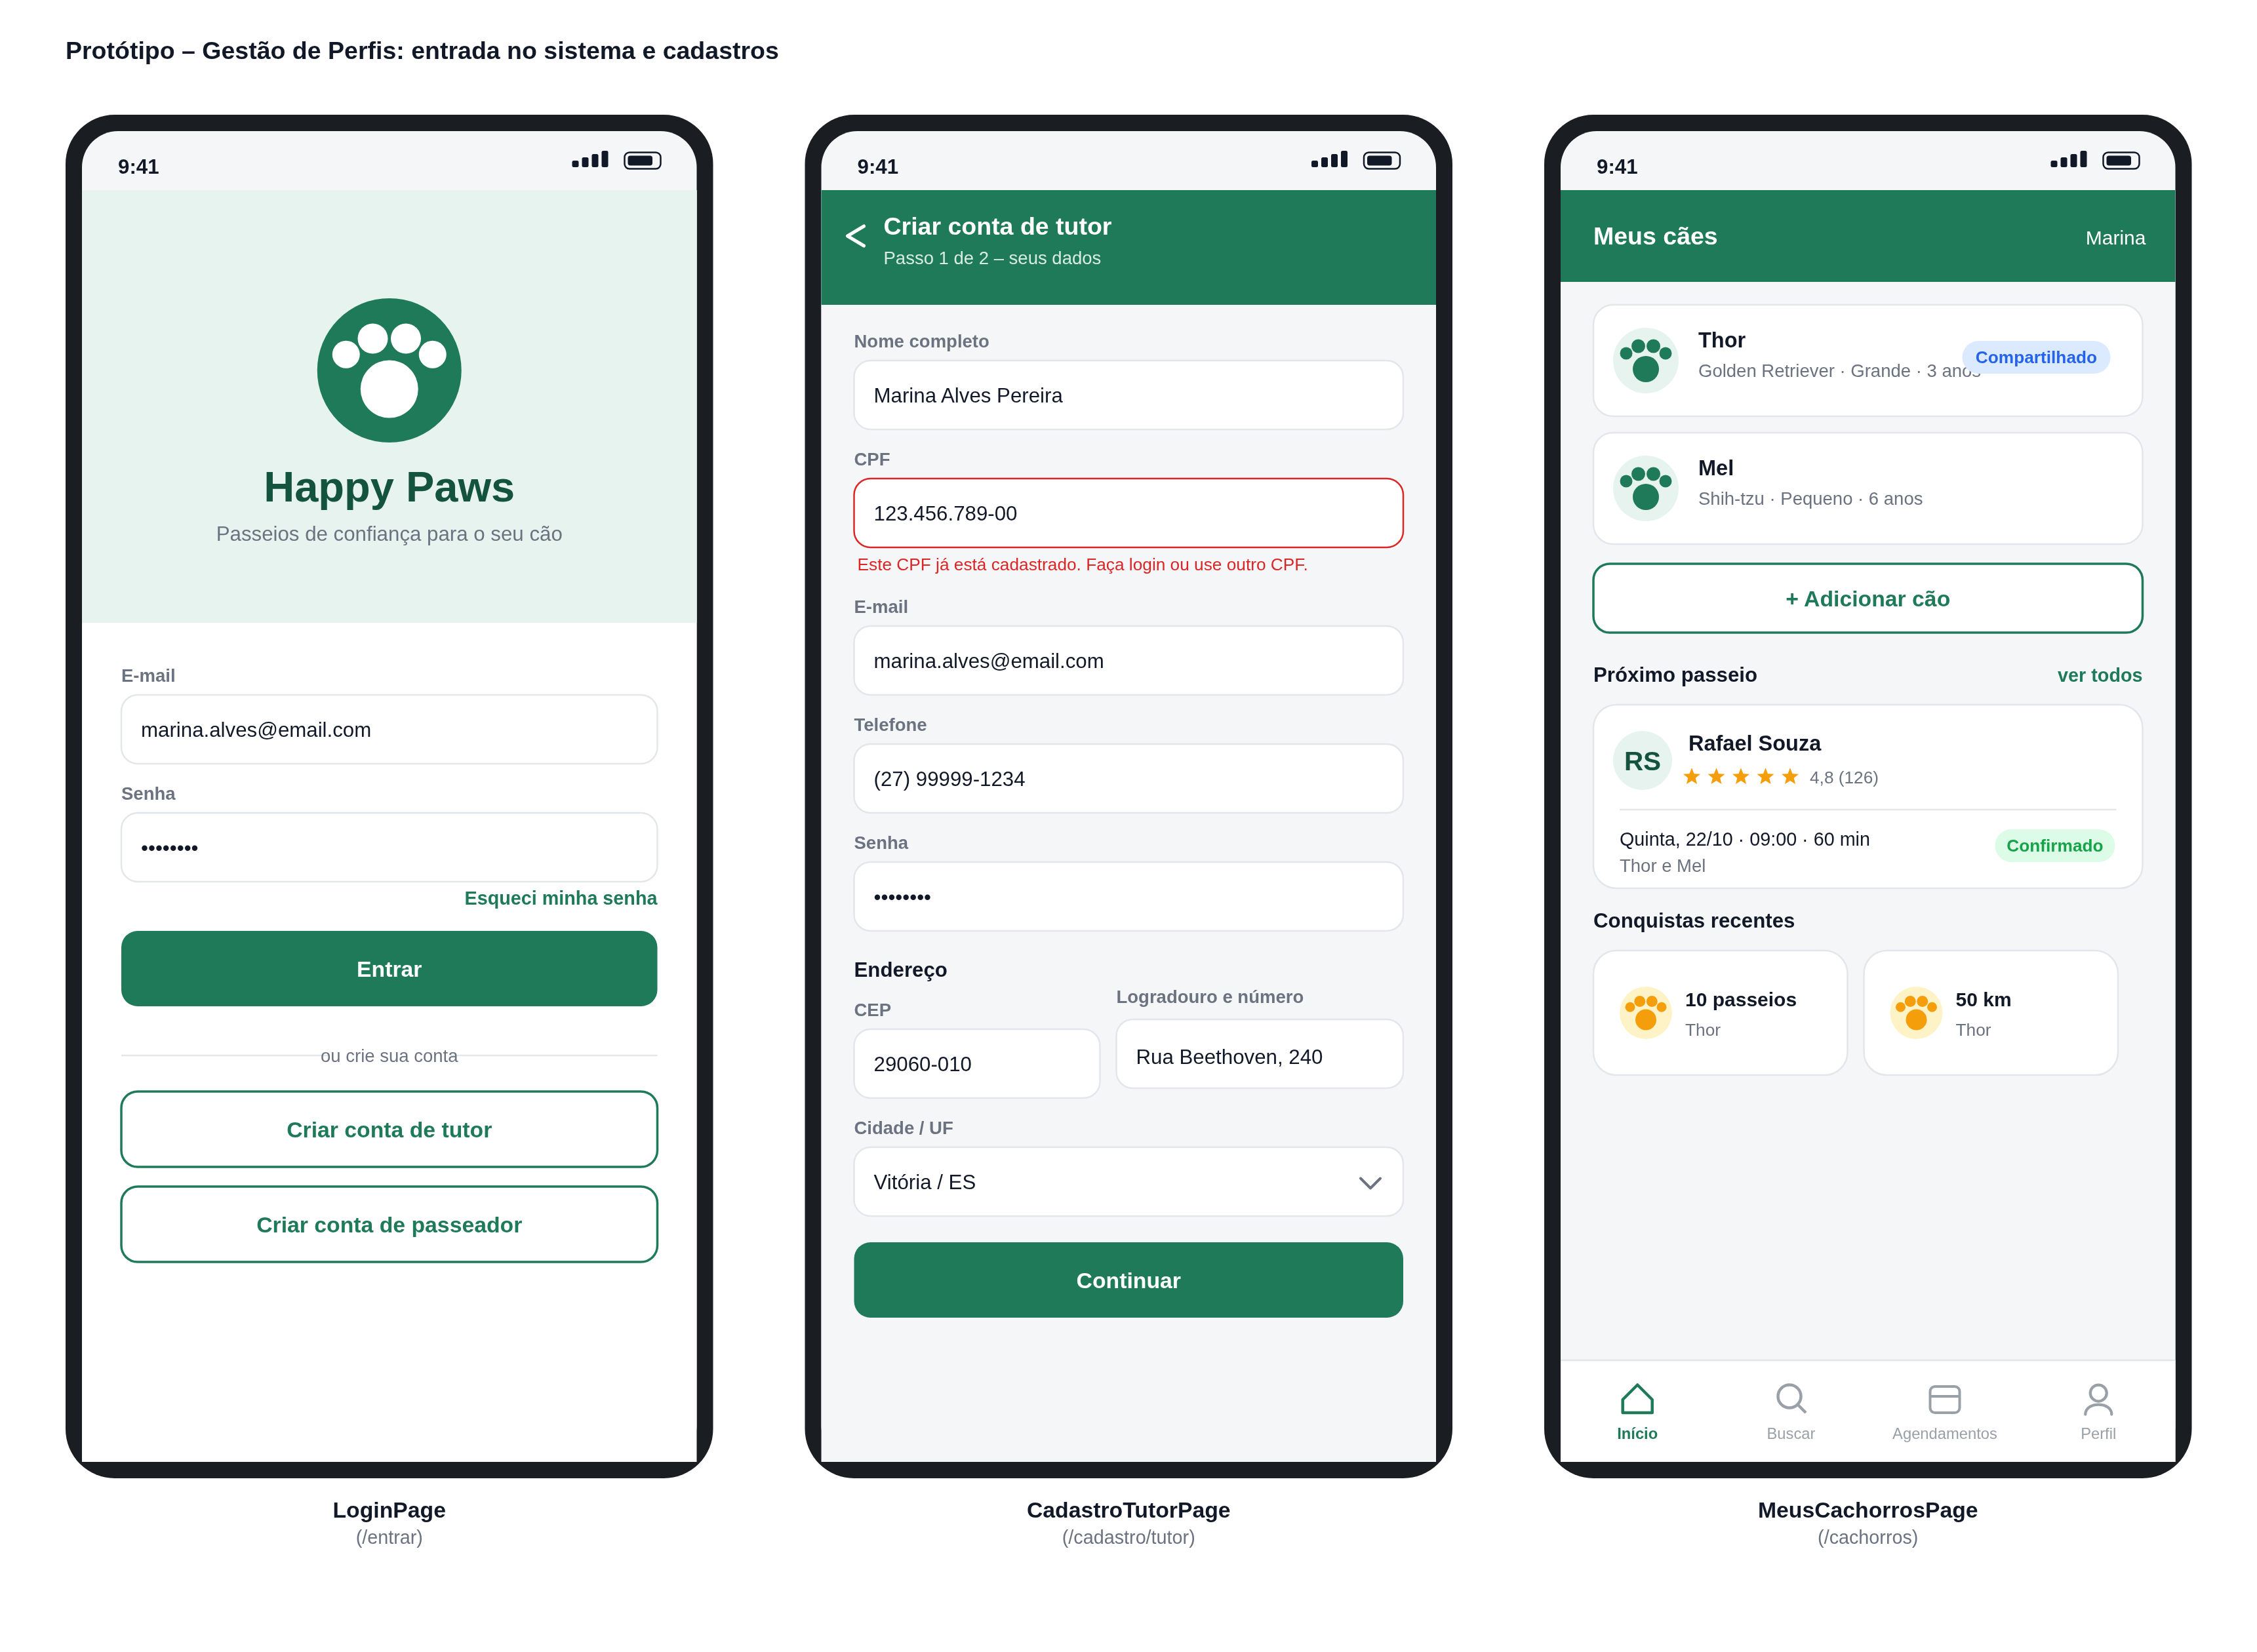
\includegraphics[width=1\textwidth,height=0.85\textheight,keepaspectratio]{figuras/proto-folha-perfis-1.png}
	\caption{Protótipo do subsistema Gestão de Perfis: entrada no sistema e cadastros.}
	\label{figura-proto-perfis-1}
\end{figure}

\begin{figure}[htbp]
	\centering
	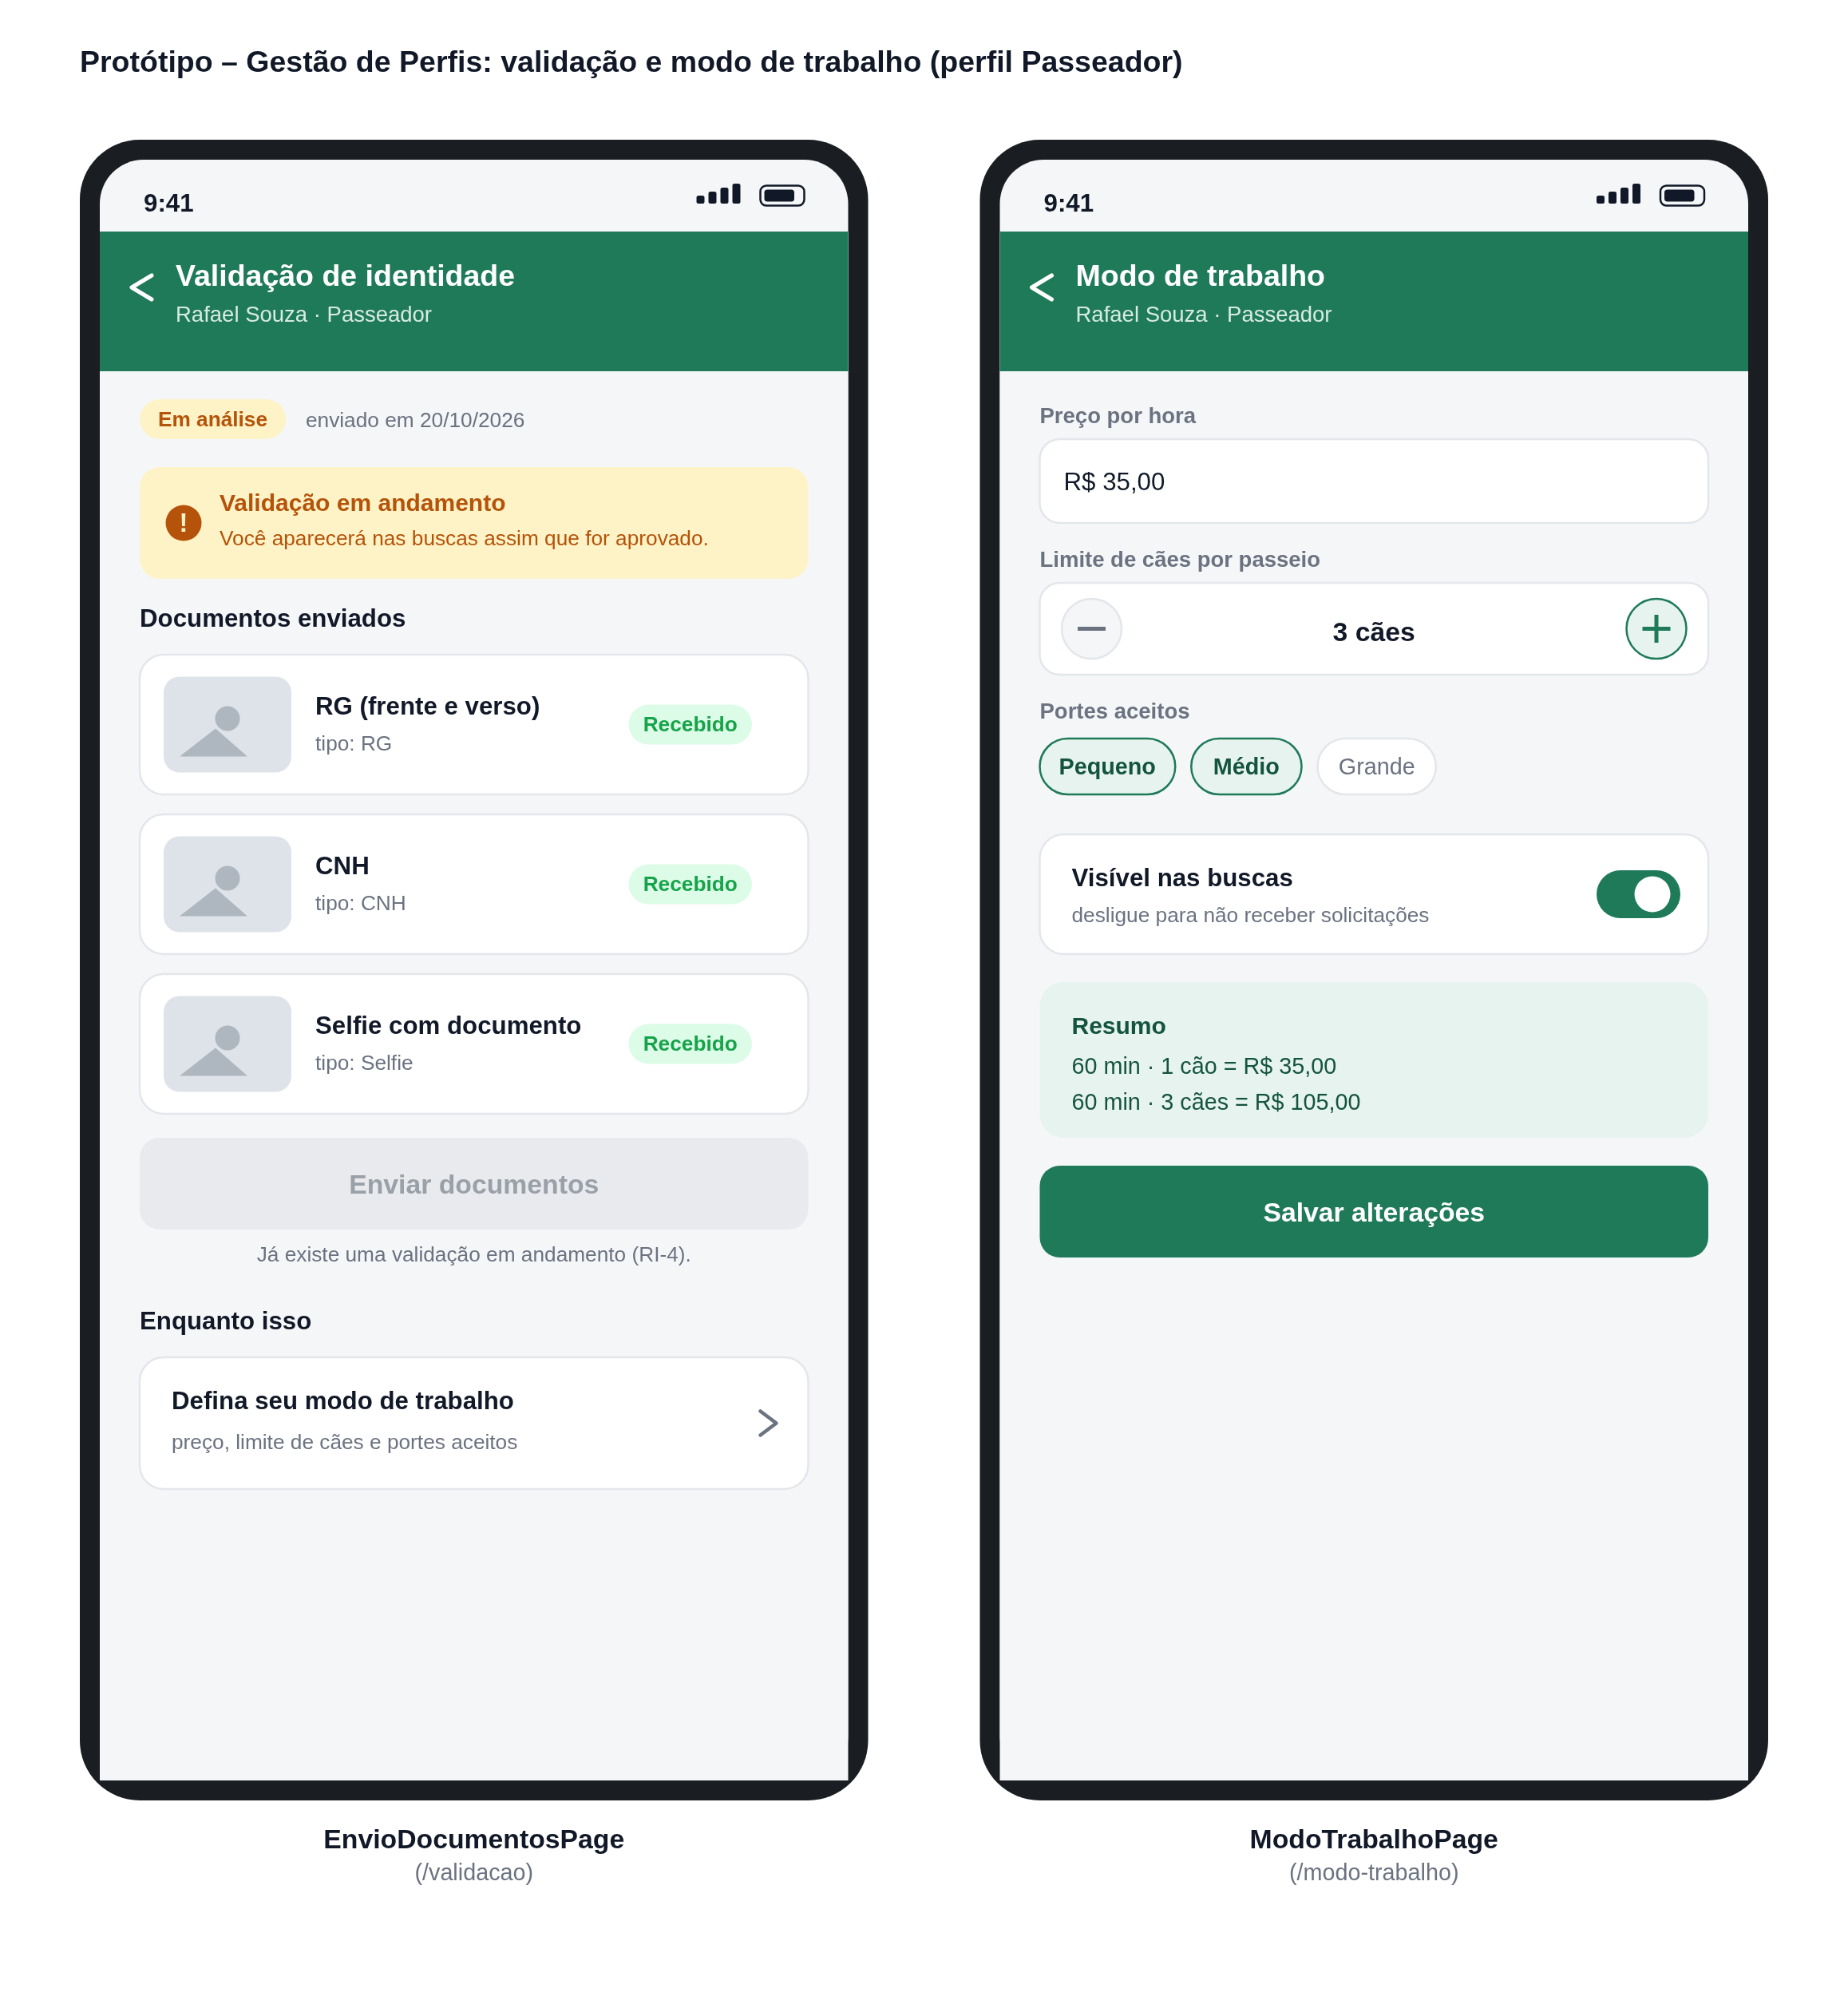
\includegraphics[width=0.68\textwidth,height=0.85\textheight,keepaspectratio]{figuras/proto-folha-perfis-2.png}
	\caption{Protótipo do subsistema Gestão de Perfis: validação de identidade e modo de trabalho (perfil Passeador).}
	\label{figura-proto-perfis-2}
\end{figure}

% ------------------------------------------------------------- Serviços
\begin{figure}[htbp]
	\centering
	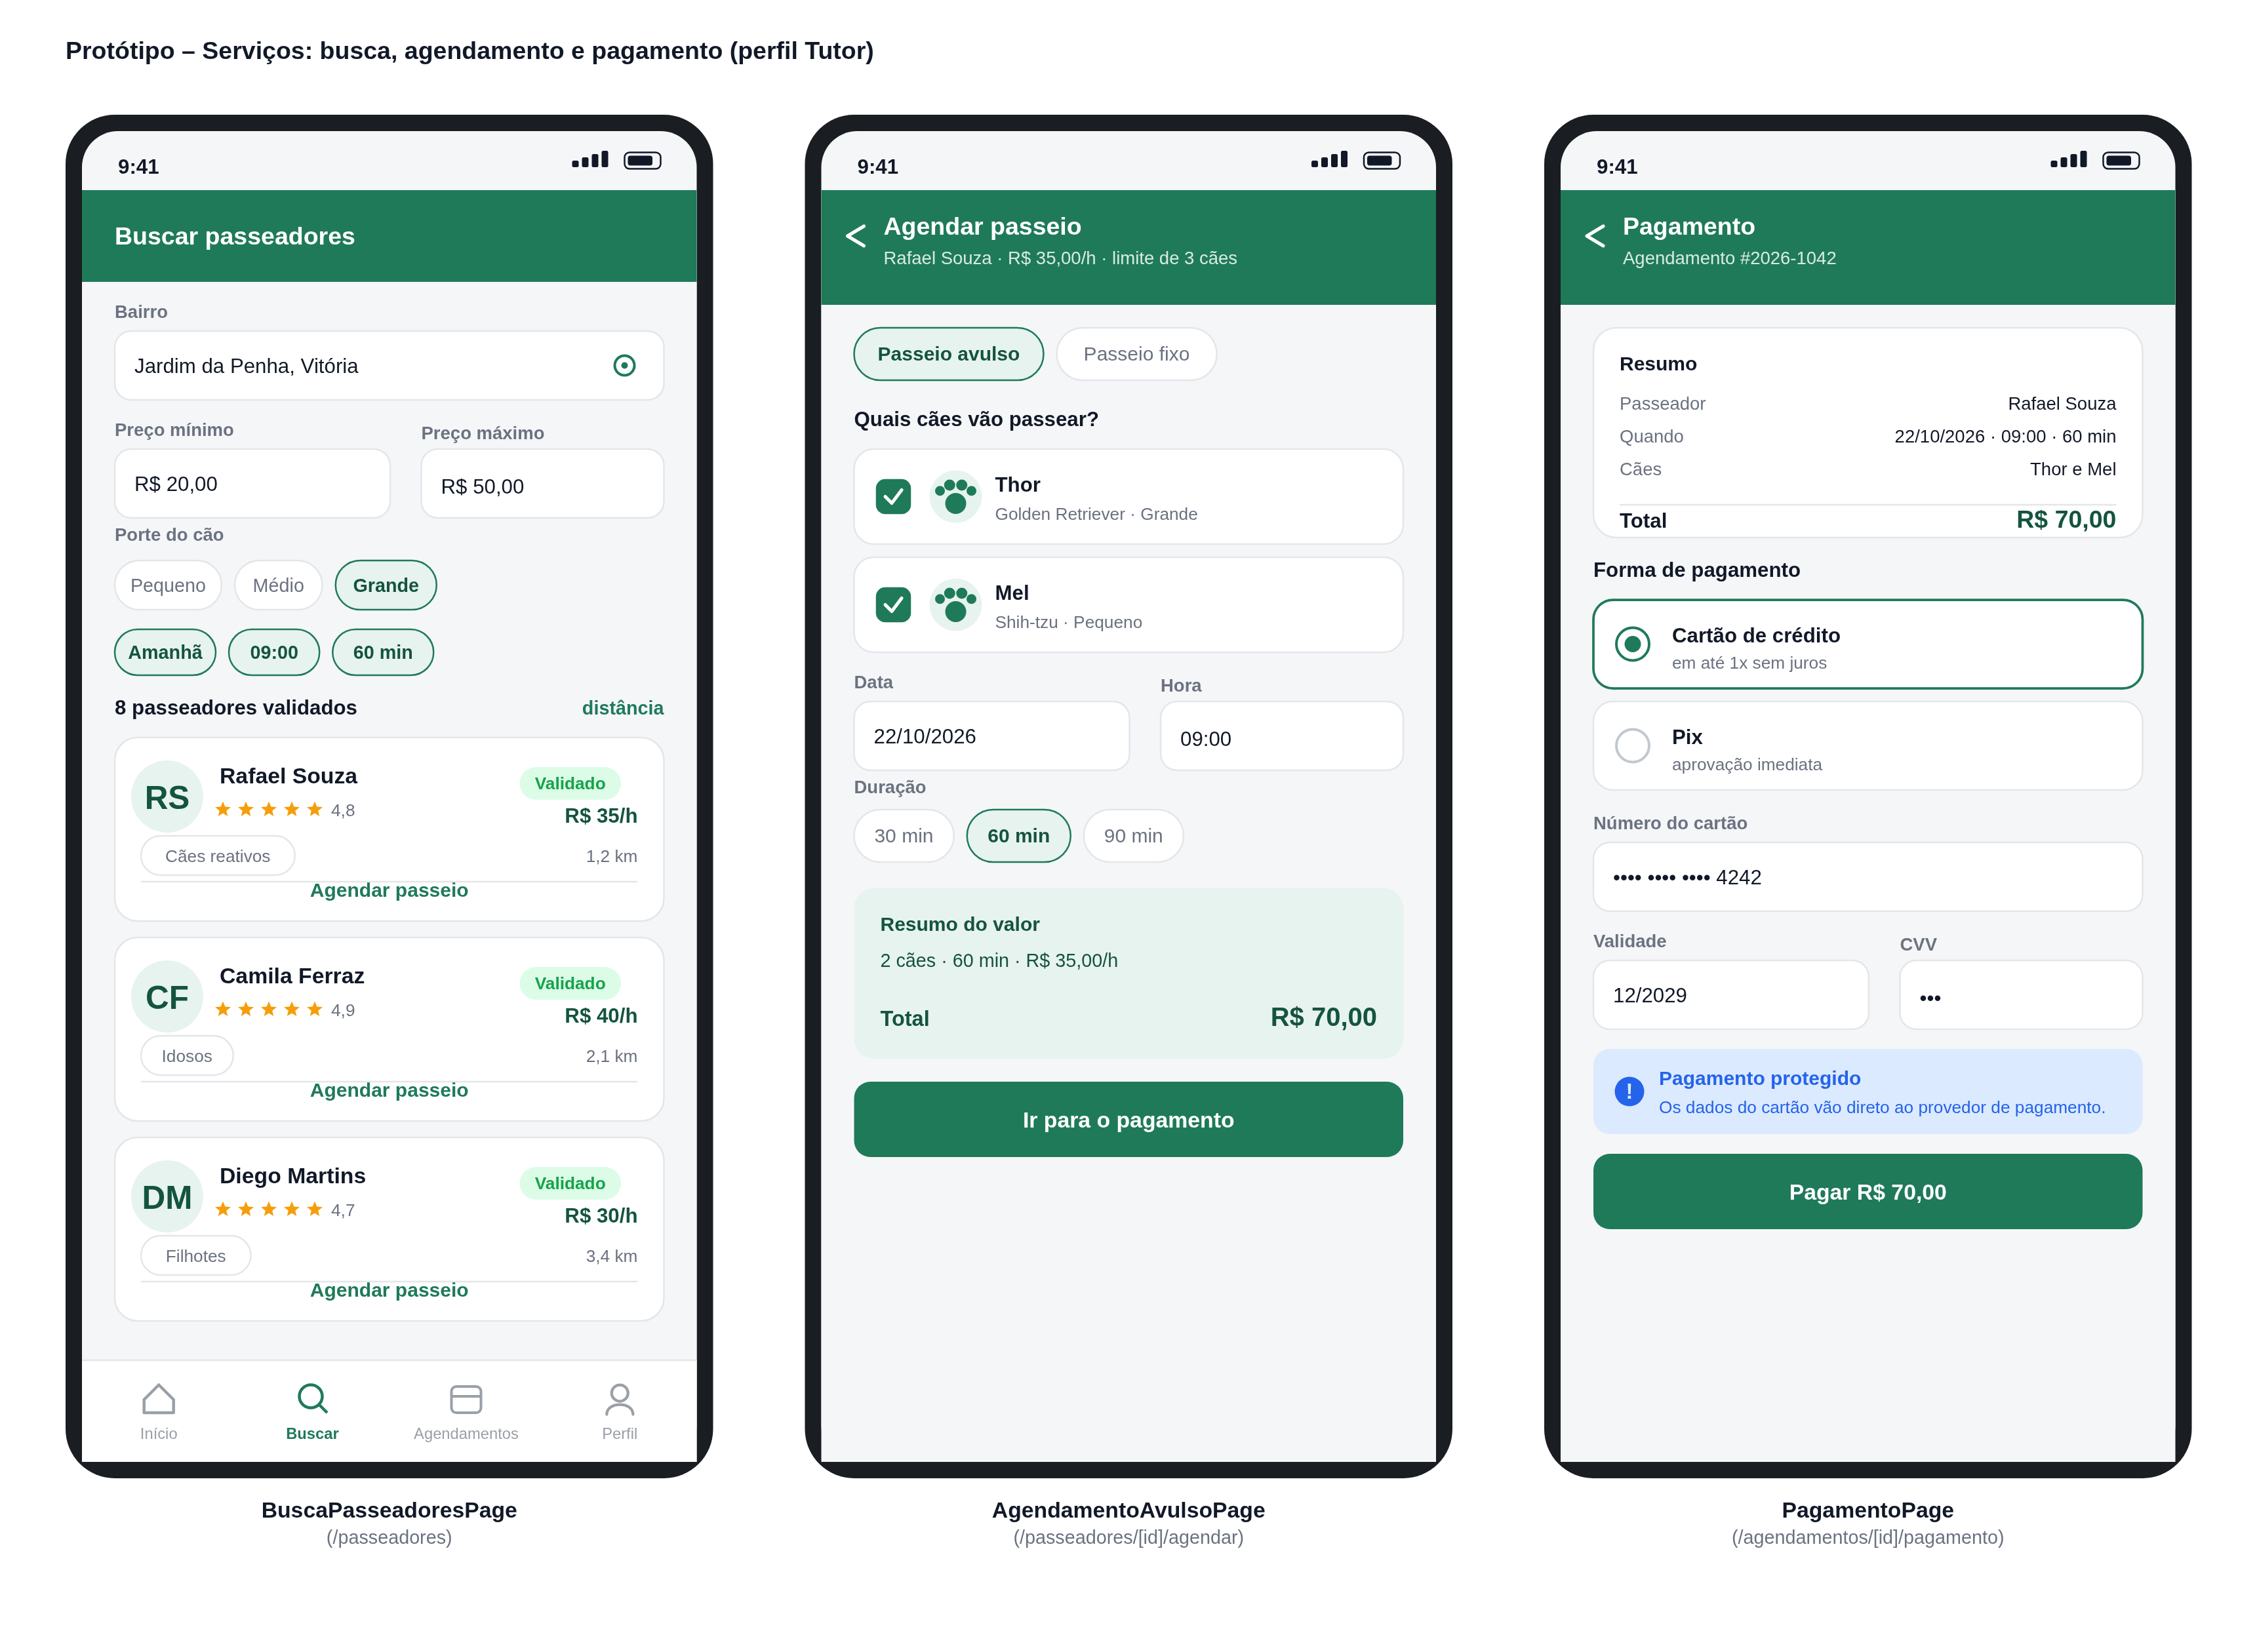
\includegraphics[width=1\textwidth,height=0.85\textheight,keepaspectratio]{figuras/proto-folha-servicos-1.png}
	\caption{Protótipo do subsistema Serviços: busca de passeadores, agendamento e pagamento (perfil Tutor).}
	\label{figura-proto-servicos-1}
\end{figure}

\begin{figure}[htbp]
	\centering
	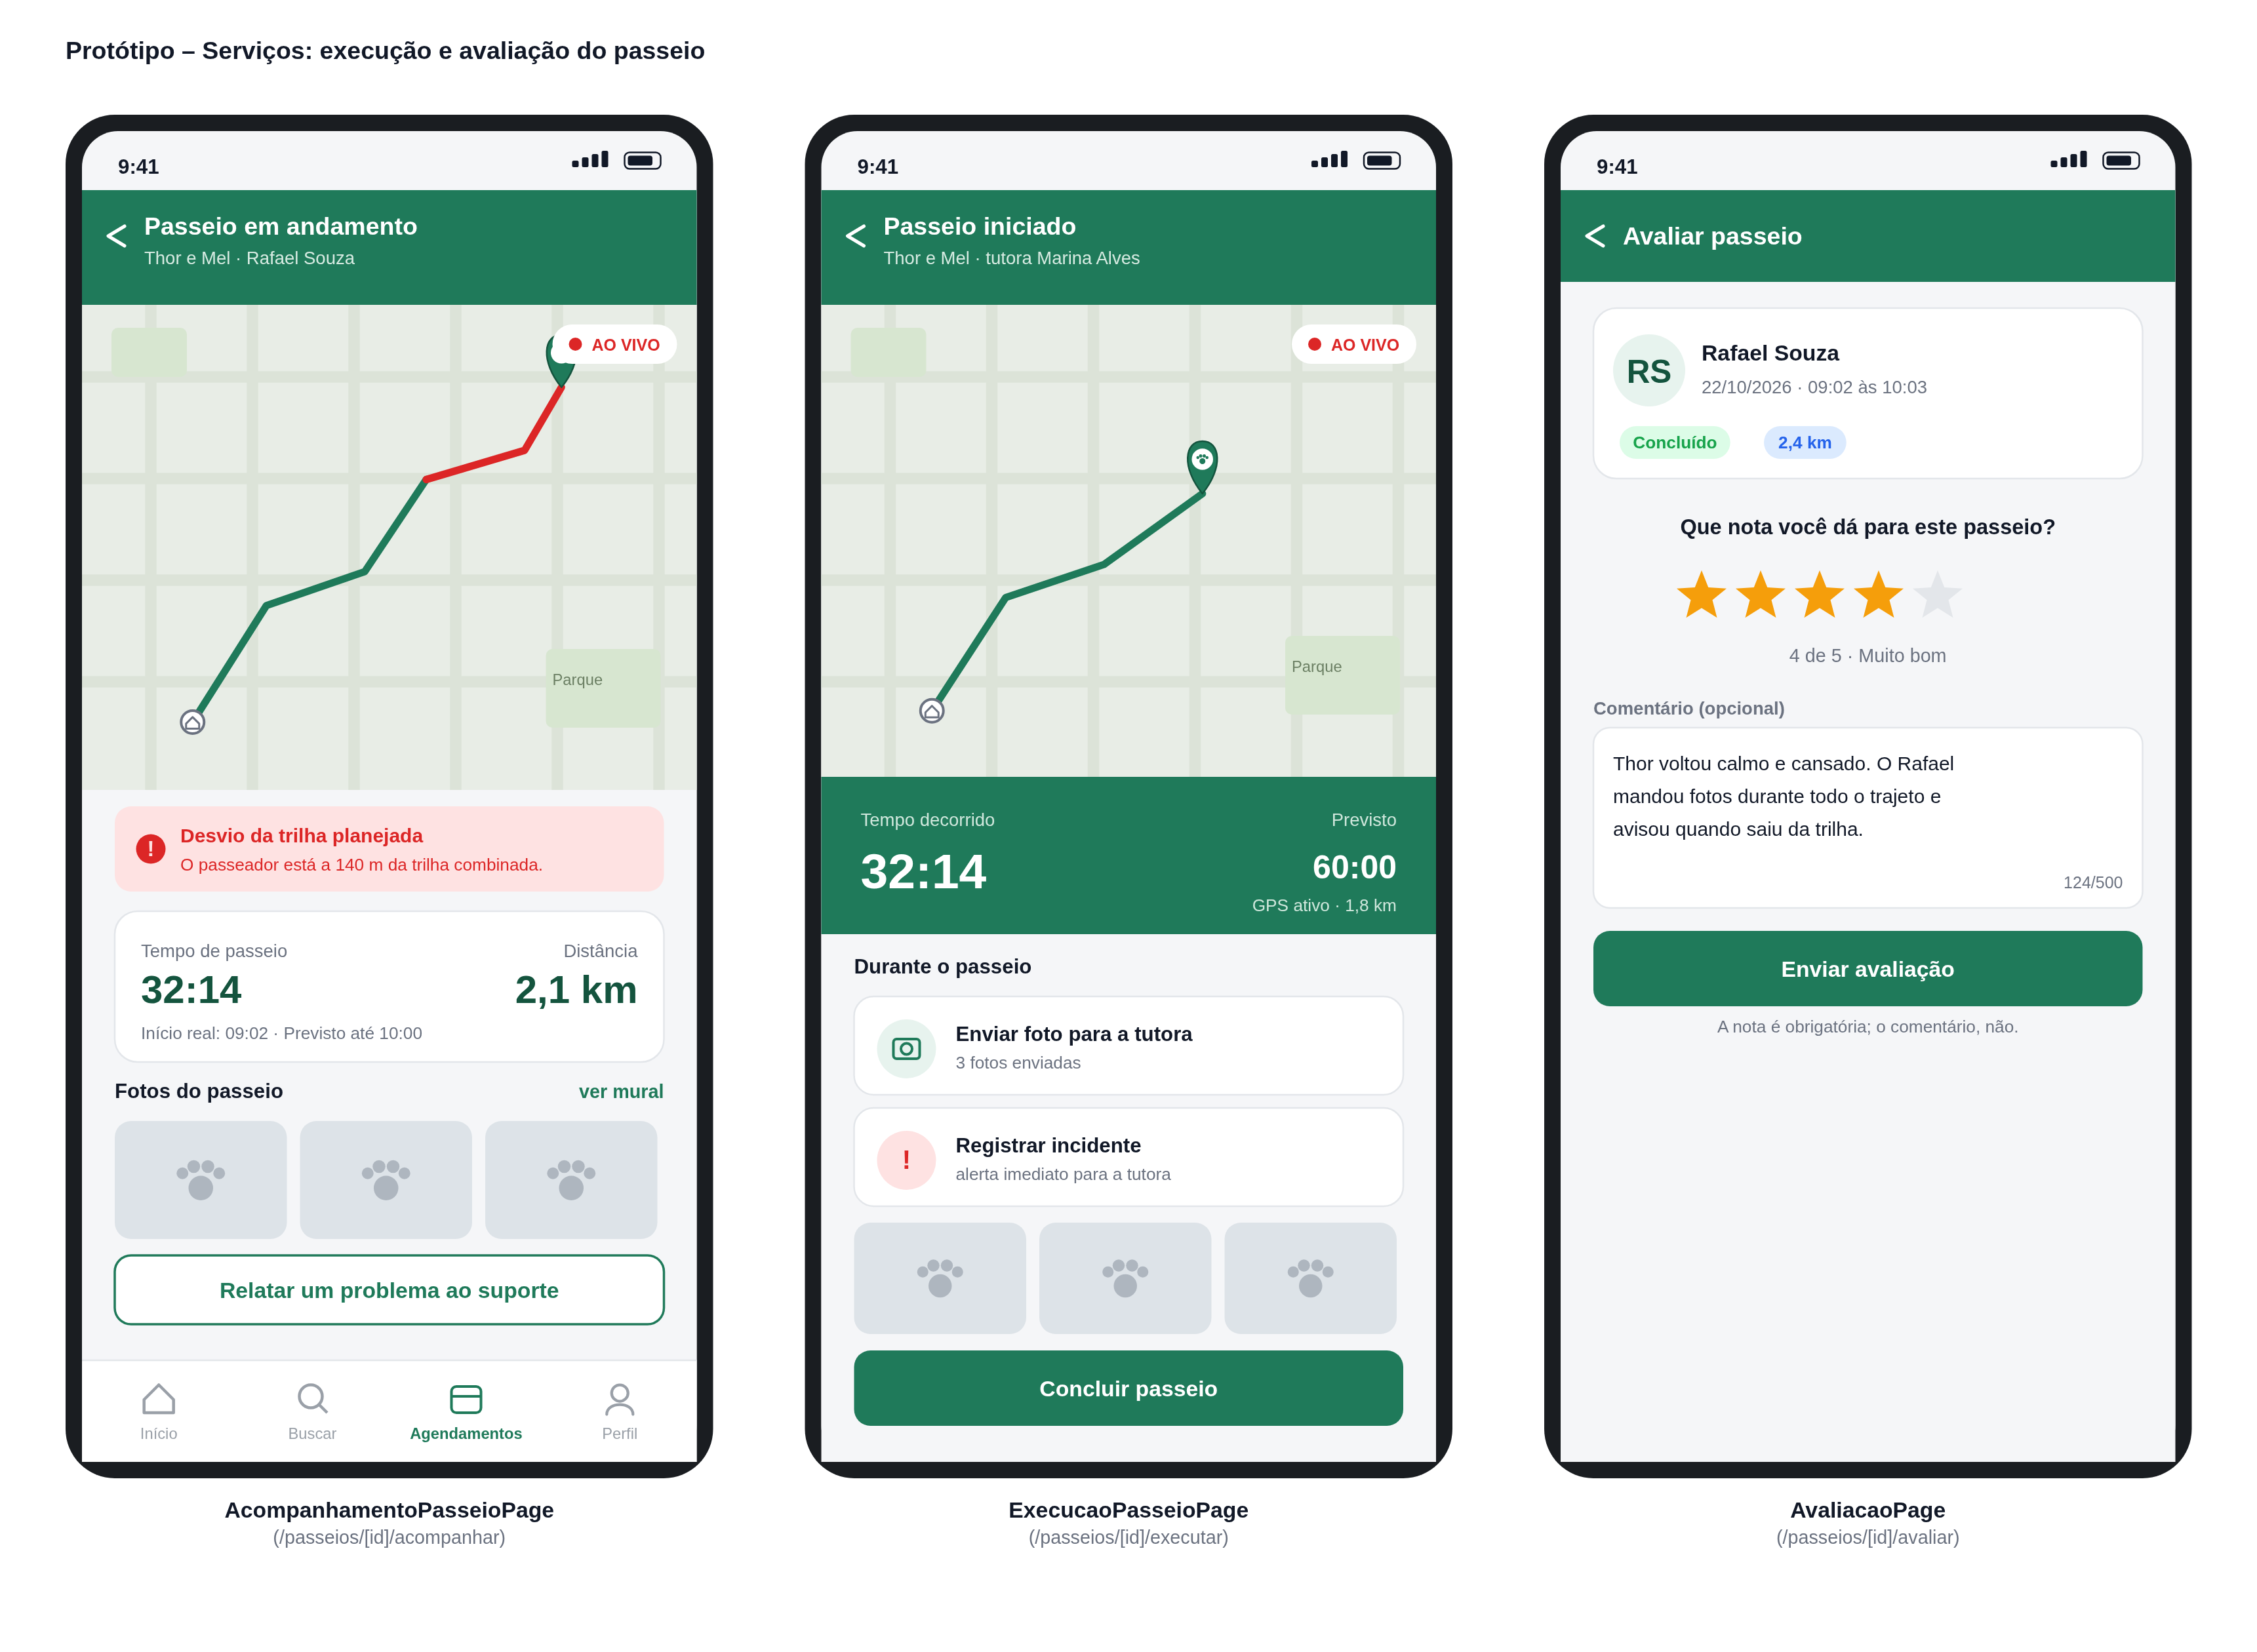
\includegraphics[width=1\textwidth,height=0.85\textheight,keepaspectratio]{figuras/proto-folha-servicos-2.png}
	\caption{Protótipo do subsistema Serviços: acompanhamento em tempo real, execução do passeio e avaliação.}
	\label{figura-proto-servicos-2}
\end{figure}

% -------------------------------------------------------------- Suporte
\begin{figure}[htbp]
	\centering
	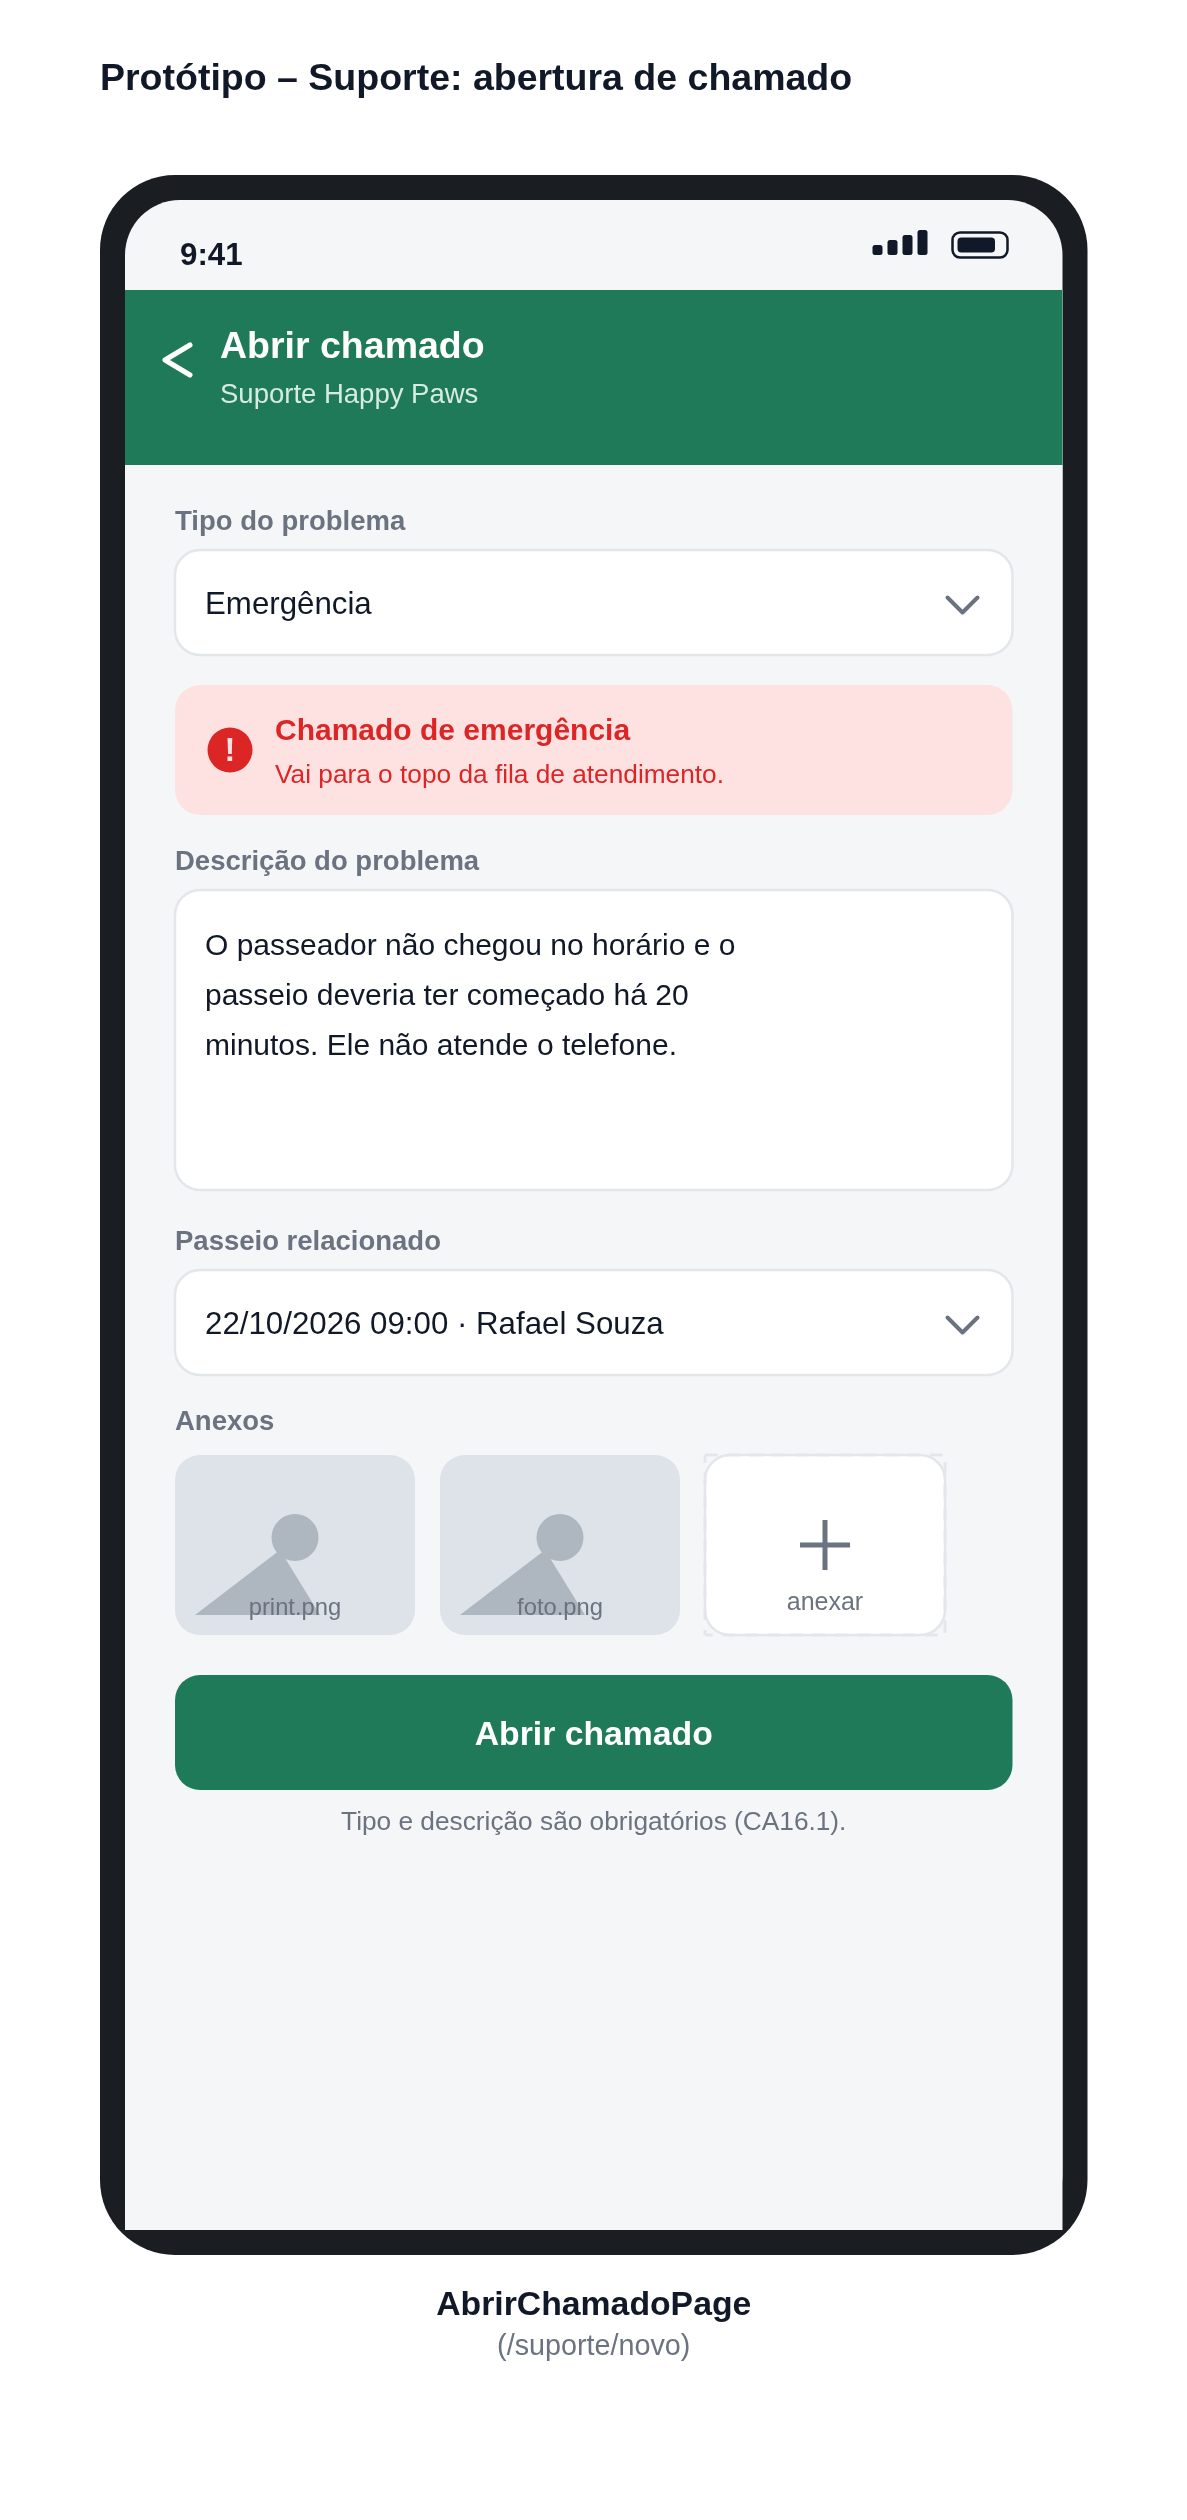
\includegraphics[width=0.29\textwidth,height=0.85\textheight,keepaspectratio]{figuras/proto-folha-suporte.png}
	\caption{Protótipo do subsistema Suporte: abertura de chamado pelo Tutor ou pelo Passeador.}
	\label{figura-proto-suporte}
\end{figure}

\begin{figure}[htbp]
	\centering
	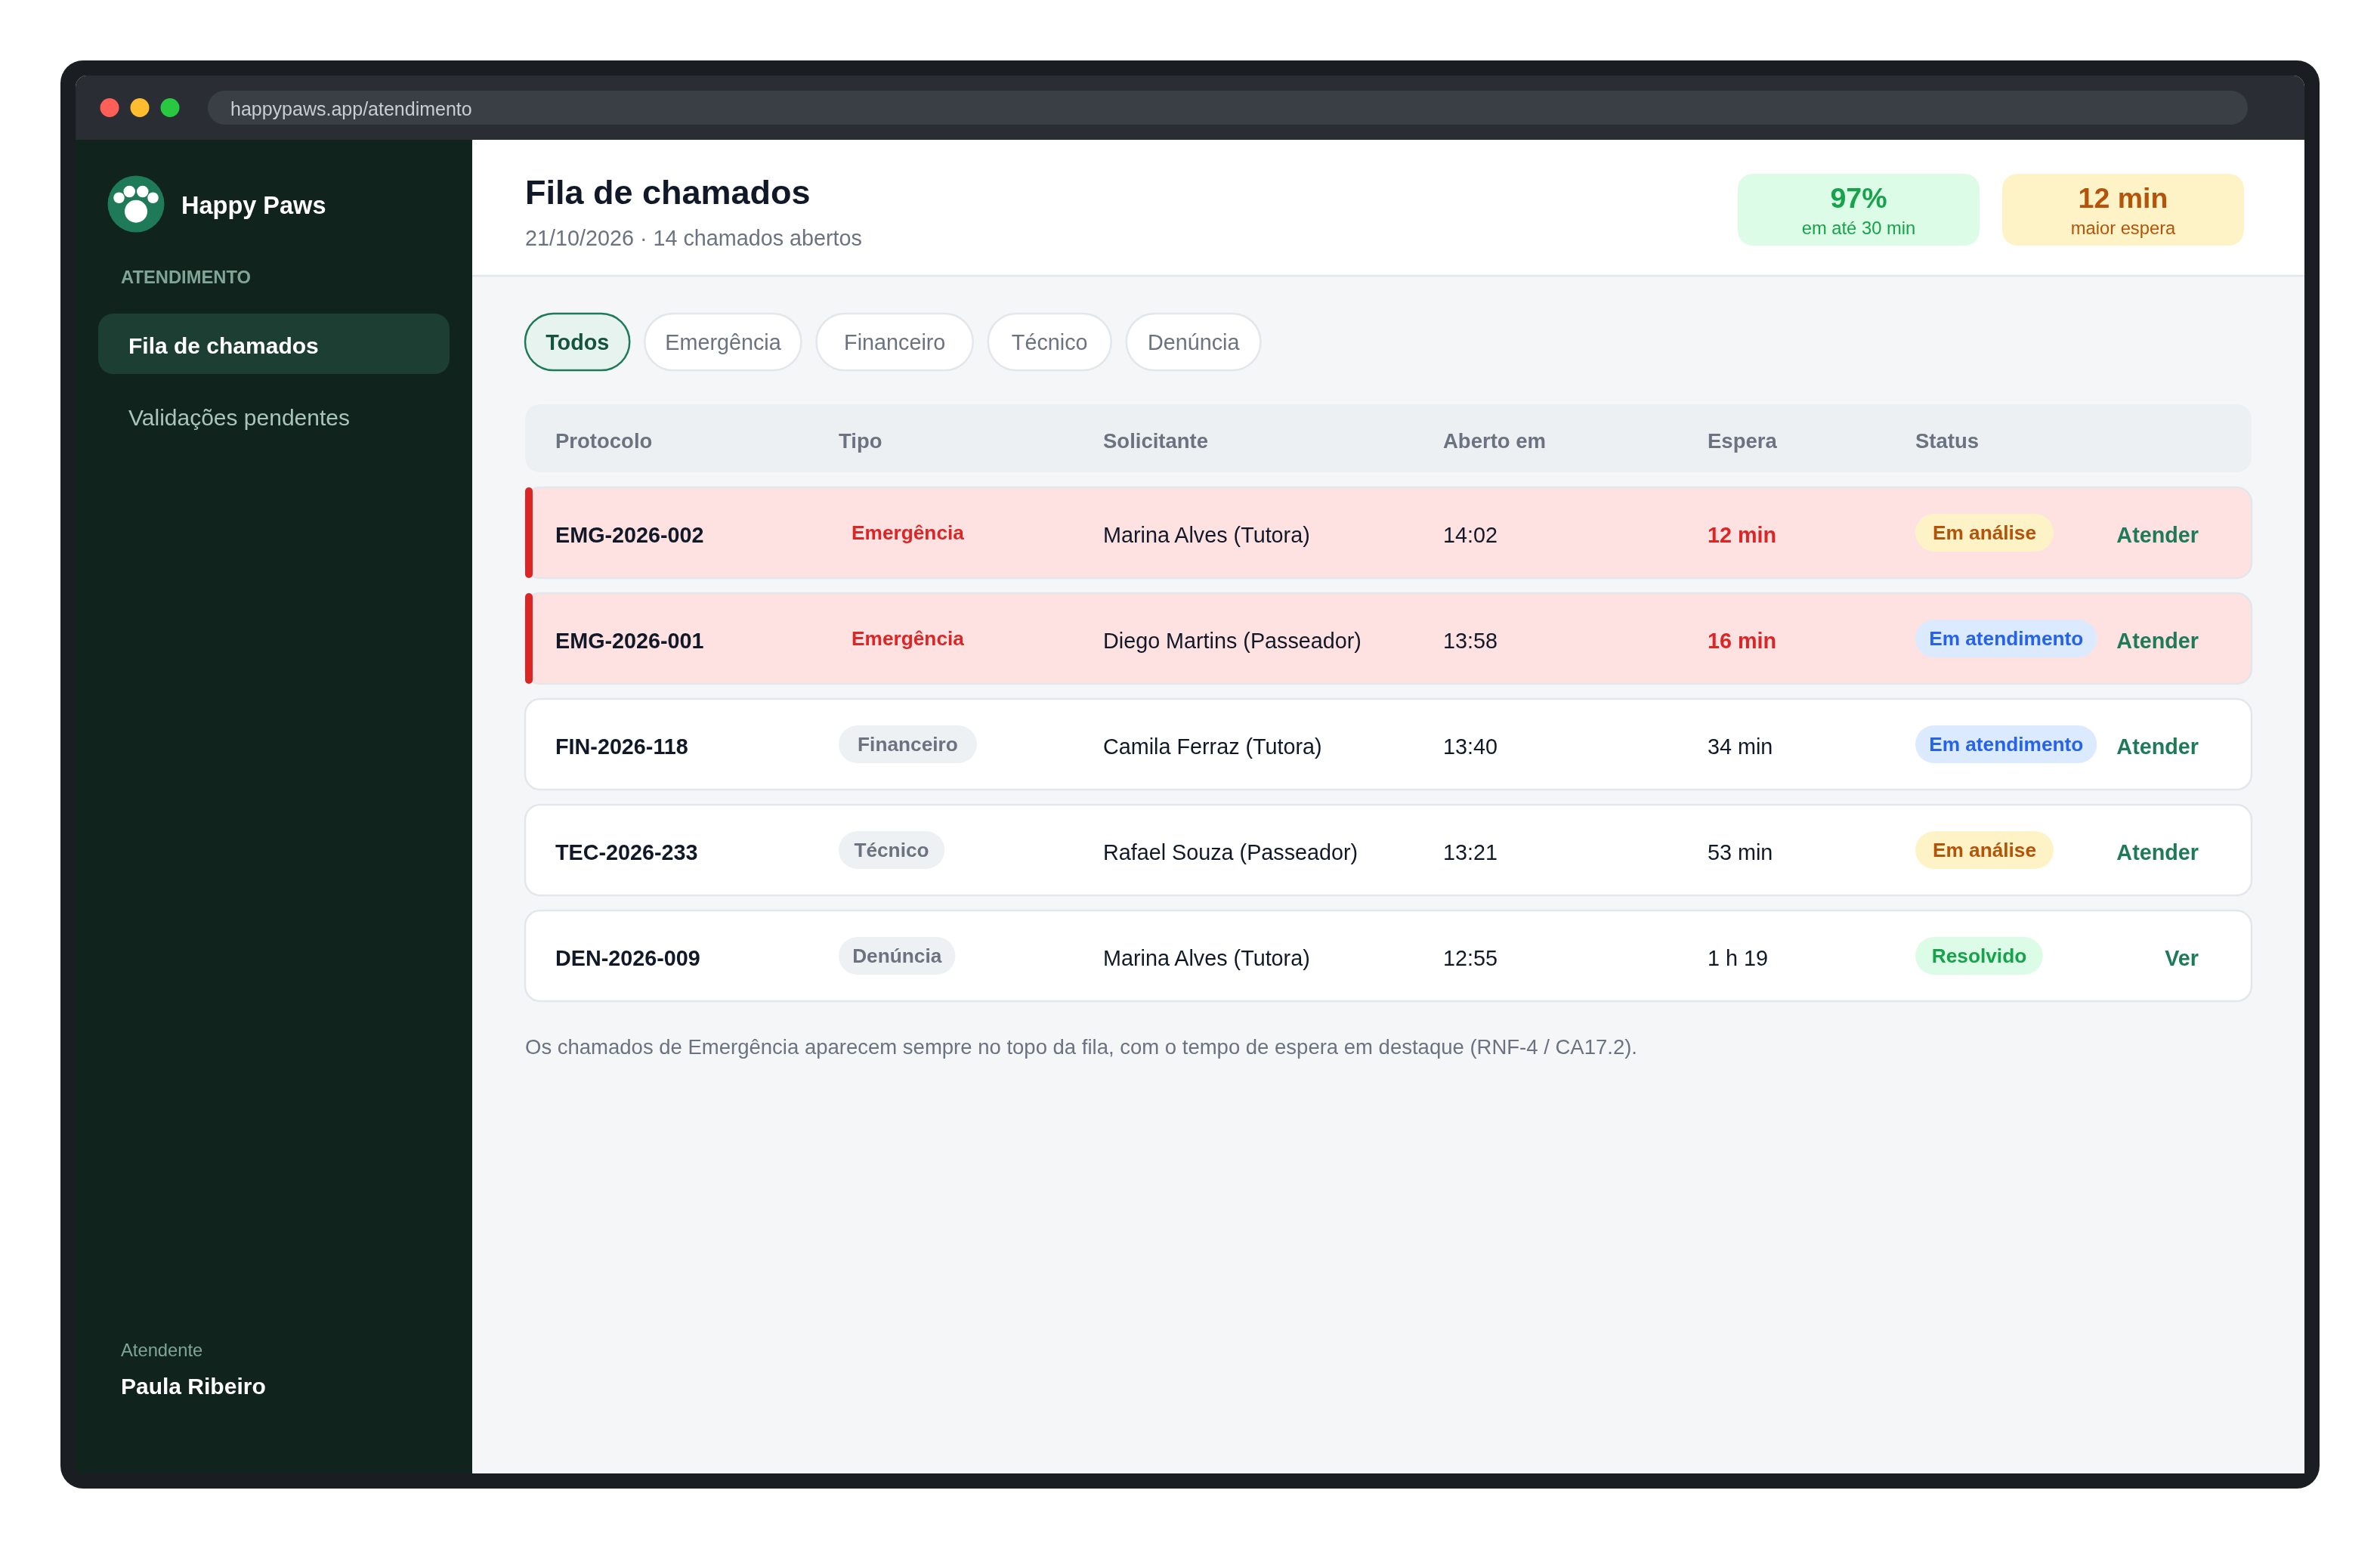
\includegraphics[width=1\textwidth,height=0.85\textheight,keepaspectratio]{figuras/proto-tela-13-fila-atendimento.png}
	\caption{Protótipo da central de atendimento (perfil Atendente): fila de chamados.}
	\label{figura-proto-fila}
\end{figure}

\begin{figure}[htbp]
	\centering
	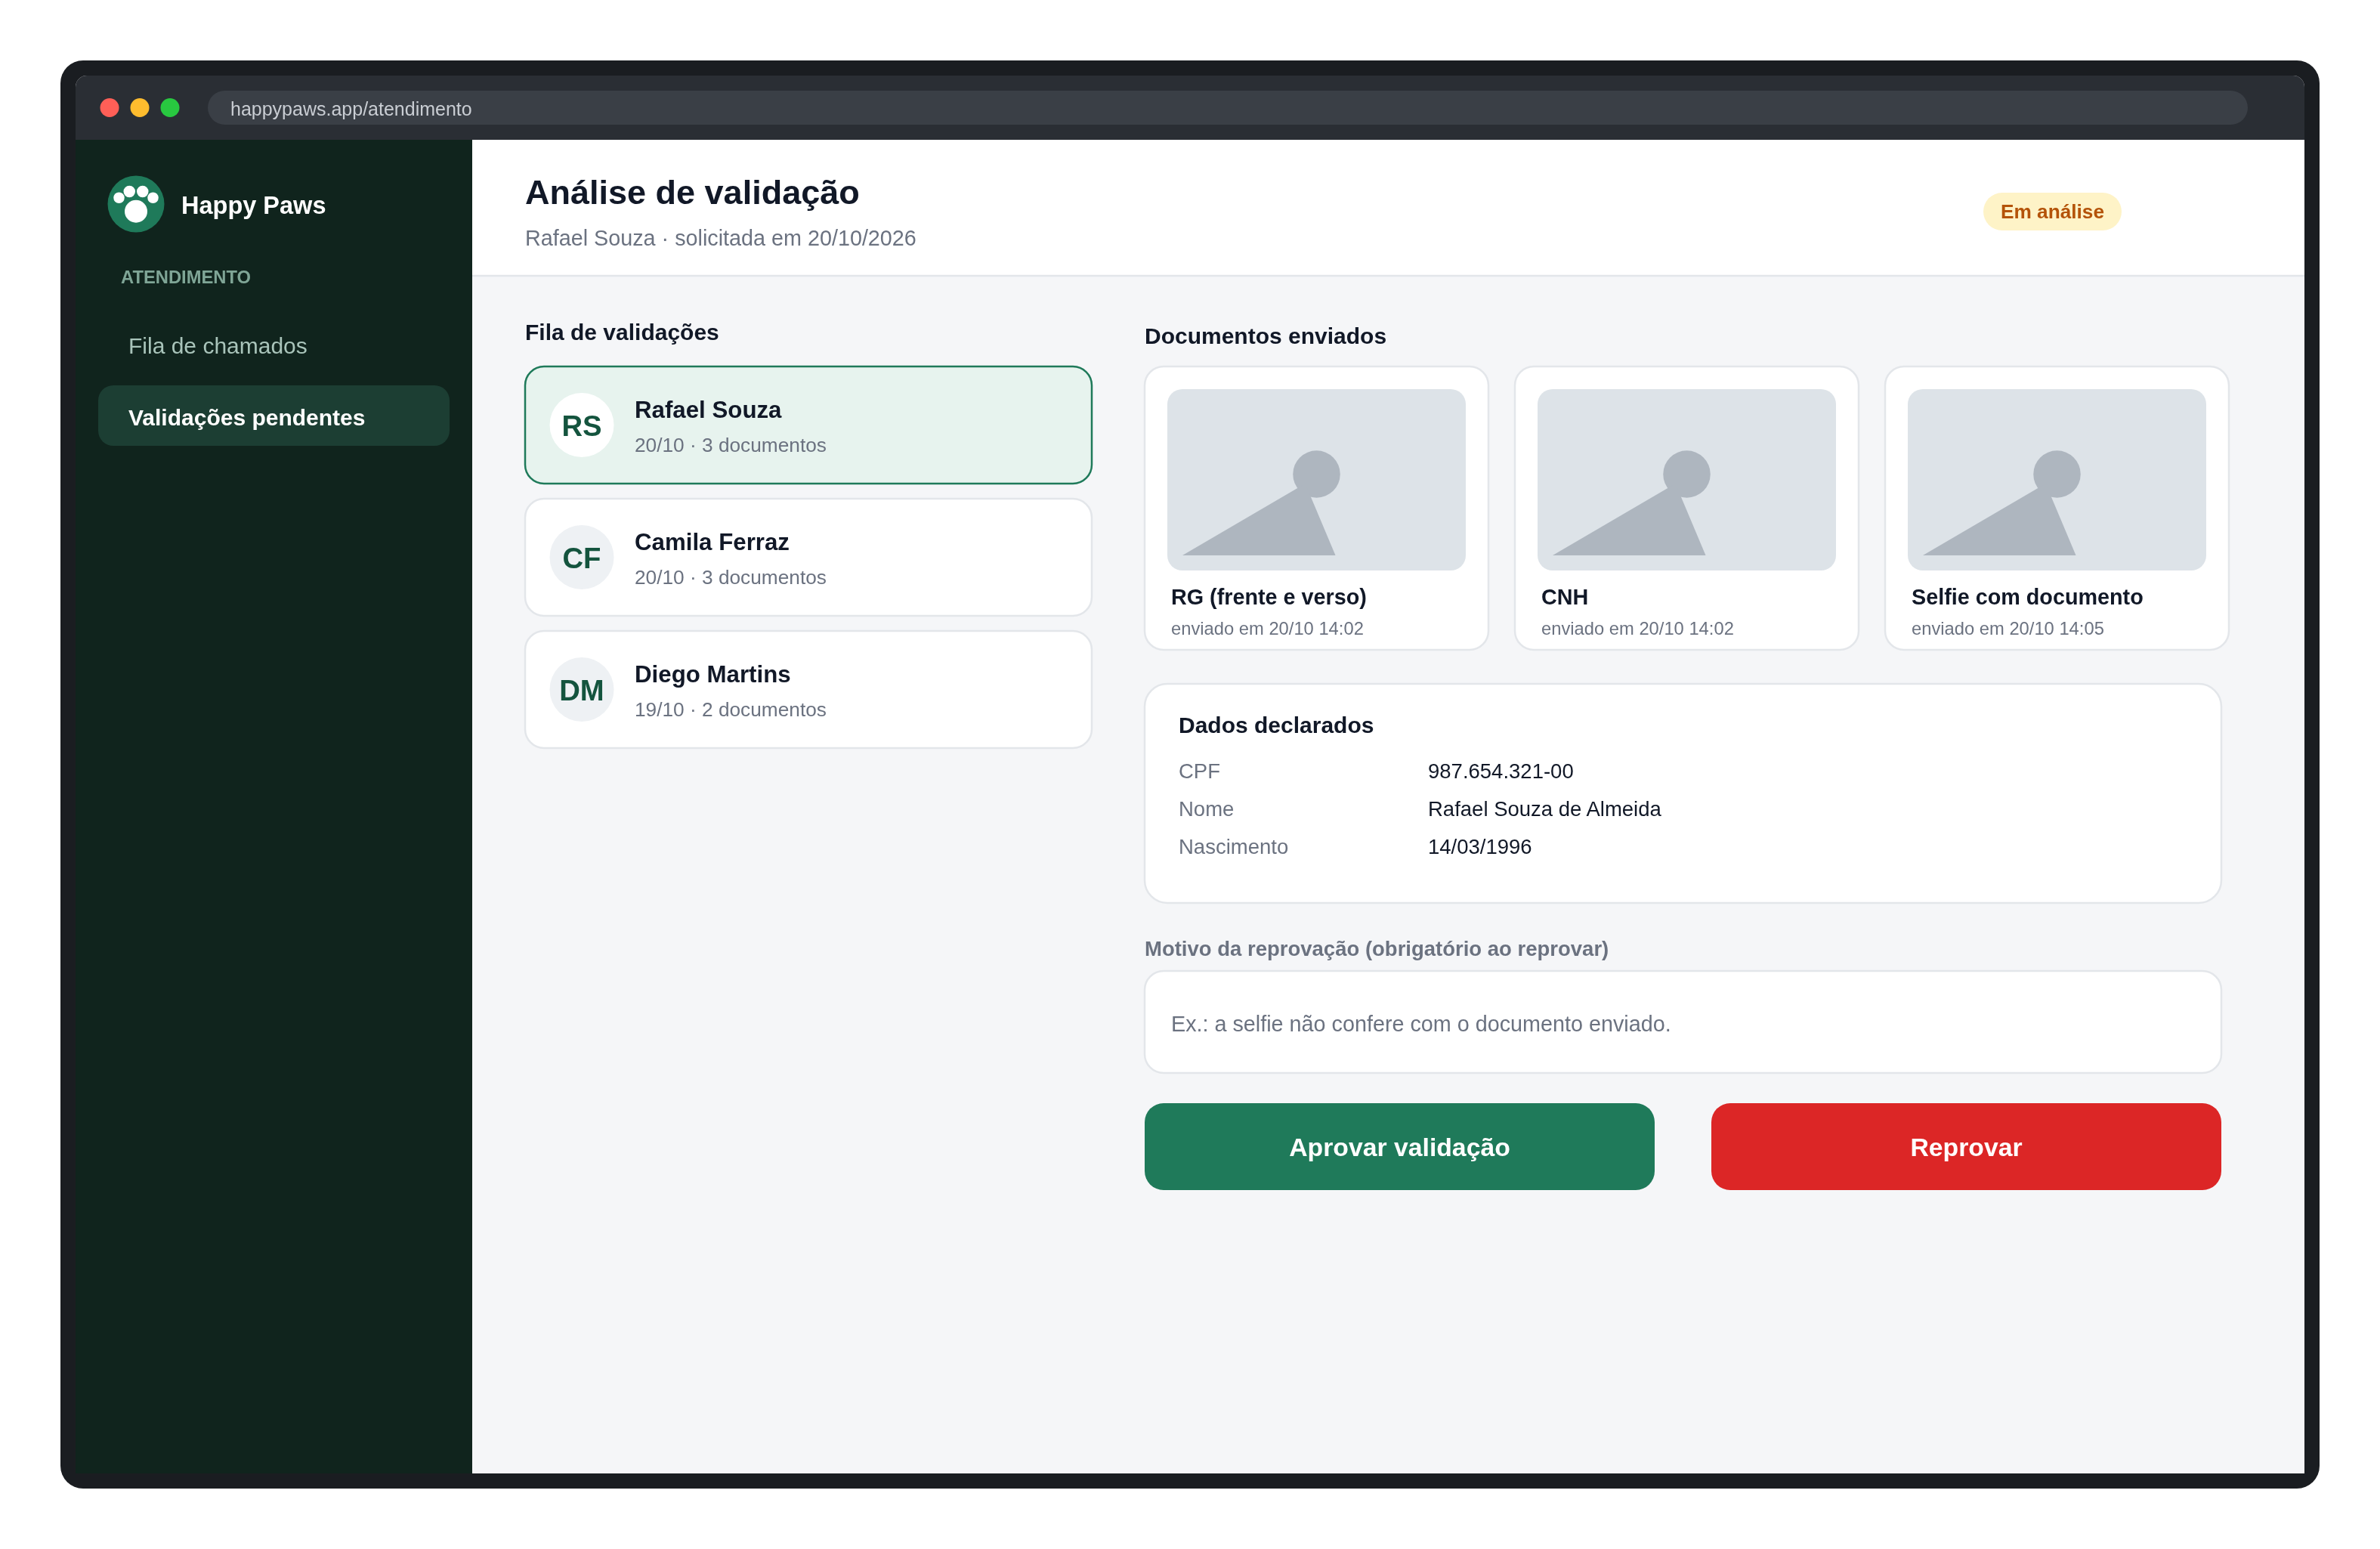
\includegraphics[width=1\textwidth,height=0.85\textheight,keepaspectratio]{figuras/proto-tela-14-analise-validacao.png}
	\caption{Protótipo da central de atendimento (perfil Atendente): análise de validação de identidade do Passeador.}
	\label{figura-proto-validacao}
\end{figure}

As decisões de projeto da interface registradas no protótipo são as seguintes:

\begin{sloppypar}
\begin{itemize}
	\item \textbf{Mensagens de erro junto ao campo.} Em \texttt{CadastroTutorPage} (Figura~\ref{figura-proto-perfis-1}), o erro de CPF já cadastrado (RI-1) aparece abaixo do próprio campo, em linguagem do usuário e com a ação sugerida, e não em uma mensagem genérica no topo da página;

	\item \textbf{Comandos inapropriados desabilitados.} Em \texttt{EnvioDocumentosPage} (Figura~\ref{figura-proto-perfis-2}), o botão de envio fica desabilitado enquanto houver uma validação em andamento (RI-4), e o motivo é informado logo abaixo do botão. A mesma tática vale para o botão ``Iniciar passeio'', que só é habilitado com o pagamento confirmado (CA14.5);

	\item \textbf{Entrada por seleção.} Porte, especialidades, portes aceitos, duração, tipo de agendamento, método de pagamento, tipo de documento e tipo de chamado são escolhidos em listas, botões de opção ou \textit{chips}, nunca digitados (Tabela~\ref{tabela-enumerados}); a localização da busca é obtida pela \textit{Geolocation API} e os cães do agendamento vêm da lista de cães do próprio Tutor;

	\item \textbf{Resumo antes do compromisso.} As telas de agendamento e de pagamento (Figura~\ref{figura-proto-servicos-1}) mostram o valor calculado por \texttt{Agendamento.calcularValor()} antes de o Tutor confirmar, e a tela de pagamento informa que os dados do cartão são enviados diretamente ao provedor de pagamento (RNF-2);

	\item \textbf{Estado do sistema sempre visível.} A tela de acompanhamento (Figura~\ref{figura-proto-servicos-2}) tem o indicador ``AO VIVO'', o tempo decorrido, a distância percorrida e o aviso de desvio de rota em destaque; o trecho fora da trilha planejada aparece em vermelho no mapa (CA10.3);

	\item \textbf{Telas de uso em movimento.} A tela de execução do passeio (perfil Passeador) usa poucos comandos, botões grandes, alto contraste e nenhuma digitação obrigatória: o cronômetro e os comandos de foto, de incidente e de conclusão ocupam toda a largura da tela;

	\item \textbf{Iniciativa do sistema na fila de atendimento.} Em \texttt{FilaAtendimentoPage} (Figura~\ref{figura-proto-fila}), os chamados do tipo ``Emergência'' aparecem no topo, com faixa e tempo de espera em destaque, e o indicador de primeiro atendimento em até 30 minutos fica no cabeçalho (RNF-4 e CA17.2);

	\item \textbf{Dados obrigatórios no momento certo.} Na análise de validação (Figura~\ref{figura-proto-validacao}), o campo de motivo fica junto dos botões e é obrigatório apenas quando o Atendente reprova a validação (CA04.4); na avaliação do passeio, a nota é obrigatória e o comentário é opcional.
\end{itemize}
\end{sloppypar}

Em relação ao protótipo de Engenharia de Software I, esta versão acrescenta as telas do perfil Atendente (fila de chamados e análise de validação), separa as páginas por rota e por perfil, conforme as Tabelas~\ref{tabela-ciu-perfis} a~\ref{tabela-ciu-suporte}, e incorpora as táticas de usabilidade da Tabela~\ref{tabela-taticas-usabilidade}.

O protótipo completo desta revisão pode ser visto na Web em \url{https://raw.githack.com/Eduardo-Ferraz/happy-paws-go/main/docs/es2-projeto/prototipo/index.html}. Os arquivos ficam no repositório do projeto, em \url{https://github.com/Eduardo-Ferraz/happy-paws-go/tree/main/docs/es2-projeto/prototipo}, em formato vetorial (SVG), uma tela por arquivo, nomeadas pela página correspondente do pacote \texttt{cih}.



%=======================================================================================================
\FloatBarrier
\section{Subsistema Gestão de Perfis}
\label{sec-ihc-perfis}

A Figura~\ref{figura-ciu-perfis} mostra o projeto da Camada de Interface com o Usuário (pacotes \texttt{cih} e \texttt{cci}) do subsistema Gestão de Perfis, juntamente com as classes de aplicação do pacote \texttt{cgt} das quais os controladores dependem (Figura~\ref{figura-ln-perfis-cgt}). As telas correspondem às Figuras 1 a 7 do documento de requisitos. A Tabela~\ref{tabela-ciu-perfis} lista as páginas, suas rotas, os perfis que as acessam e os controladores responsáveis.

\begin{figure}[h]
	\centering
	\figciu{figuras/ciu-perfis.png}{0.85}
	\caption{Projeto da Camada de Interface com o Usuário (\texttt{cih} e \texttt{cci}) do subsistema Gestão de Perfis.}
	\label{figura-ciu-perfis}
\end{figure}

\begin{scriptsize}
\setlength{\tabcolsep}{3pt}
\begin{longtable}{|p{4.2cm}|p{3.6cm}|p{1.7cm}|p{1.3cm}|p{3.8cm}|}
	\caption{Páginas do subsistema Gestão de Perfis.}
	\label{tabela-ciu-perfis}\\\hline
	\rowcolor{lightgray}
	\textbf{Página} & \textbf{Rota} & \textbf{Perfil} & \textbf{US} & \textbf{Controlador} \\\hline
	\endfirsthead
	\hline
	\rowcolor{lightgray}
	\textbf{Página} & \textbf{Rota} & \textbf{Perfil} & \textbf{US} & \textbf{Controlador} \\\hline
	\endhead
	\texttt{LoginPage} & \texttt{/entrar} & Todos & US01, US03 & \texttt{CadastroUsuario\-Controller} \\\hline
	\texttt{CadastroTutorPage} & \texttt{/cadastro/tutor} & Visitante & US01 & \texttt{CadastroUsuario\-Controller} \\\hline
	\texttt{CadastroPasseadorPage} & \texttt{/cadastro/\allowbreak passeador} & Visitante & US03 & \texttt{CadastroUsuario\-Controller} \\\hline
	\texttt{EditarPerfilPage} & \texttt{/perfil} & Tutor, Passeador & US01, US03 & \texttt{CadastroUsuario\-Controller} \\\hline
	\texttt{MeusCachorrosPage} & \texttt{/cachorros} & Tutor & US02 & \texttt{CadastroCachorro\-Controller} \\\hline
	\texttt{CadastroCachorroPage} & \texttt{/cachorros/novo} e \texttt{/cachorros/\allowbreak [id]/editar} & Tutor & US02 & \texttt{CadastroCachorro\-Controller} \\\hline
	\texttt{CompartilharPerfilPage} & \texttt{/cachorros/\allowbreak [id]/compartilhar} & Tutor & US05 & \texttt{Compartilhamento\-PerfilController} \\\hline
	\texttt{ConvitesPage} & \texttt{/convites} & Tutor & US05 & \texttt{Compartilhamento\-PerfilController} \\\hline
	\texttt{EnvioDocumentosPage} & \texttt{/validacao} & Passeador & US04 & \texttt{ValidacaoPasseador\-Controller} \\\hline
	\texttt{ModoTrabalhoPage} & \texttt{/modo-trabalho} & Passeador & US06 & \texttt{ModoTrabalho\-Controller} \\\hline
	\texttt{ValidacoesPendentesPage} & \texttt{/atendimento/\allowbreak validacoes} & Atendente & US04 & \texttt{ValidacaoPasseador\-Controller} \\\hline
	\texttt{AnaliseValidacaoPage} & \texttt{/atendimento/\allowbreak validacoes/[id]} & Atendente & US04 & \texttt{ValidacaoPasseador\-Controller} \\\hline
\end{longtable}
\end{scriptsize}

Os controladores se ligam às classes de aplicação do \texttt{cgt} da seguinte forma:

\begin{itemize}
	\item \texttt{CadastroUsuarioController}: \texttt{AplCadastroUsuario};
	\item \texttt{CadastroCachorroController}: \texttt{AplCadastroCachorro};
	\item \texttt{CompartilhamentoPerfilController}: \texttt{AplCompartilhamentoPerfil};
	\item \texttt{ValidacaoPasseadorController}: \texttt{AplValidacaoPasseador};
	\item \texttt{ModoTrabalhoController}: \texttt{AplModoTrabalho}.
\end{itemize}

A seguir, para fins didáticos, são explicadas as funcionalidades do subsistema:

\begin{sloppypar}
\begin{itemize}
	\item \textbf{Login:} \texttt{LoginPage} pede e-mail e senha e os envia a \texttt{CadastroUsuarioController}, que chama \texttt{AplCadastroUsuario.autenticar()} (a verificação da senha é feita pelo Better Auth). Em caso de sucesso, o controlador redireciona o usuário para a página inicial do seu perfil: \texttt{MeusCachorrosPage} (Tutor), \texttt{ModoTrabalhoPage} (Passeador) ou \texttt{ValidacoesPendentesPage} (Atendente). A página tem \textit{links} para as páginas de cadastro e para a recuperação de senha (``Esqueci minha senha''), que é feita pelo Better Auth e não corresponde a uma \textit{user story}, por isso não aparece no diagrama;
	\item \textbf{Cadastro de Tutor e de Passeador:} \texttt{CadastroTutorPage} e \texttt{CadastroPasseadorPage} pedem os dados pessoais, o endereço e, para o Passeador, a biografia, o limite de cães, os portes aceitos e as especialidades (listas de seleção). Os dados são enviados a \texttt{CadastroUsuarioController}, que chama \texttt{cadastrarTutor()} ou \texttt{cadastrarPasseador()}. Se o CPF ou o e-mail já estiverem cadastrados (RI-1 e RI-2), o erro volta para a página e é mostrado junto ao campo. Em caso de sucesso, o Tutor é redirecionado para \texttt{LoginPage} e o Passeador para \texttt{EnvioDocumentosPage};
	\item \textbf{Edição de perfil:} \texttt{EditarPerfilPage}, aberta pelo menu do \textit{layout} das áreas do Tutor e do Passeador, mostra os dados atuais (\texttt{consultarPerfil()}), permite alterá-los e os envia a \texttt{CadastroUsuarioController}, que chama \texttt{atualizarPerfil()} e volta à mesma página com uma mensagem de sucesso;
	\item \textbf{Cadastro de cães:} \texttt{MeusCachorrosPage} lista os cães do Tutor (\texttt{listarCachorros()}). O botão ``Adicionar cão'' leva a \texttt{CadastroCachorroPage}; as ações de cada cão (editar, compartilhar, que leva a \texttt{CompartilharPerfilPage}, e remover) ficam no menu do card do cão, que não aparece aberto no protótipo; a página também tem um \textit{link} para \texttt{ConvitesPage}. \texttt{CadastroCachorroPage} é usada para cadastrar e para editar (\texttt{cadastrarCachorro()} e \texttt{atualizarCachorro()}), e o porte é escolhido em uma lista; depois de salvar, o controlador volta para \texttt{MeusCachorrosPage}. A remoção (\texttt{removerCachorro()}) pede confirmação e, quando o cão tem outros Tutores, apenas desvincula o Tutor atual (RI-3);
	\item \textbf{Compartilhamento do perfil do cão:} \texttt{CompartilharPerfilPage} pede o e-mail do Tutor convidado e o envia a \texttt{CompartilhamentoPerfilController}, que chama \texttt{convidarTutor()}. O convidado vê os convites pendentes em \texttt{ConvitesPage} (\texttt{listarConvites()}), onde pode aceitar ou recusar cada um (\texttt{aceitarConvite()} e \texttt{recusarConvite()}); ao aceitar, o controlador o redireciona para \texttt{MeusCachorrosPage}, onde o cão passa a aparecer;
	\item \textbf{Validação de identidade:} em \texttt{EnvioDocumentosPage}, o Passeador escolhe o tipo de cada documento (RG, CNH, Selfie ou CPF, conforme a Tabela~\ref{tabela-enumerados}), anexa os arquivos e os envia a \texttt{ValidacaoPasseadorController}, que chama \texttt{enviarDocumentos()}. A página mostra o estado da validação mais recente (\texttt{consultarValidacao()}: ``Em Análise'', ``Validado'' ou ``Reprovado'', com o motivo) e, se já houver validação em andamento, o envio fica desativado (RI-4). Enquanto aguarda a análise, o Passeador pode seguir o \textit{link} para \texttt{ModoTrabalhoPage}. O Atendente vê em \texttt{ValidacoesPendentesPage} as validações pendentes (\texttt{listarValidacoesPendentes()}), abre uma delas em \texttt{AnaliseValidacaoPage} (que repete a lista de pendentes na lateral, para o Atendente passar de uma validação a outra sem voltar), visualiza os documentos e escolhe entre aprovar (\texttt{aprovarValidacao()}) e reprovar, caso em que o motivo é obrigatório (\texttt{reprovarValidacao()}, CA04.4). Depois da decisão, o controlador volta para \texttt{ValidacoesPendentesPage};
	\item \textbf{Modo de trabalho:} \texttt{ModoTrabalhoPage} carrega os dados atuais (\texttt{consultarModoTrabalho()}) e permite alterar o preço por hora, o limite de cães e os portes aceitos, que são enviados a \texttt{ModoTrabalhoController}, que chama \texttt{configurarModoTrabalho()}. A chave de visibilidade nas buscas chama \texttt{alterarDisponibilidade()} e tem efeito imediato. As duas operações são de \texttt{AplModoTrabalho}. Valores inválidos (por exemplo, preço negativo) são recusados e mostrados na própria página (CA06.2). O preço é digitado em reais e convertido para centavos antes do envio.
\end{itemize}
\end{sloppypar}


%=======================================================================================================
\FloatBarrier
\section{Subsistema Serviços}
\label{sec-ihc-servicos}

A Figura~\ref{figura-ciu-servicos} mostra o projeto da Camada de Interface com o Usuário do subsistema Serviços, juntamente com as classes de aplicação do \texttt{cgt} (Figura~\ref{figura-ln-servicos-cgt}) e a interface \texttt{NotificadorTempoReal}. As telas correspondem às Figuras 8 a 24 do documento de requisitos. A Tabela~\ref{tabela-ciu-servicos} lista as páginas e os controladores.

\begin{figure}[h]
	\centering
	\figciu{figuras/ciu-servicos.png}{0.85}
	\caption{Projeto da Camada de Interface com o Usuário (\texttt{cih} e \texttt{cci}) do subsistema Serviços.}
	\label{figura-ciu-servicos}
\end{figure}

\begin{scriptsize}
\setlength{\tabcolsep}{3pt}
\begin{longtable}{|p{4.2cm}|p{3.6cm}|p{1.7cm}|p{1.3cm}|p{3.8cm}|}
	\caption{Páginas do subsistema Serviços.}
	\label{tabela-ciu-servicos}\\\hline
	\rowcolor{lightgray}
	\textbf{Página} & \textbf{Rota} & \textbf{Perfil} & \textbf{US} & \textbf{Controlador} \\\hline
	\endfirsthead
	\hline
	\rowcolor{lightgray}
	\textbf{Página} & \textbf{Rota} & \textbf{Perfil} & \textbf{US} & \textbf{Controlador} \\\hline
	\endhead
	\texttt{BuscaPasseadoresPage} & \texttt{/passeadores} & Tutor & US07 & \texttt{BuscaPasseadores\-Controller} \\\hline
	\texttt{AgendamentoAvulsoPage} & \texttt{/passeadores/\allowbreak [id]/agendar} & Tutor & US08 & \texttt{Agendamento\-Controller} \\\hline
	\texttt{AgendamentoFixoPage} & \texttt{/passeadores/\allowbreak [id]/agendar-fixo} & Tutor & US09 & \texttt{Agendamento\-Controller} \\\hline
	\texttt{MeusAgendamentosPage} & \texttt{/agendamentos} & Tutor, Passeador & US08, US09 & \texttt{Agendamento\-Controller} \\\hline
	\texttt{Solicitacoes\-PendentesPage} & \texttt{/solicitacoes} & Passeador & US08, US09 & \texttt{Agendamento\-Controller} \\\hline
	\texttt{PagamentoPage} & \texttt{/agendamentos/\allowbreak [id]/pagamento} & Tutor & US14 & \texttt{Pagamento\-Controller} \\\hline
	\texttt{ExecucaoPasseioPage} & \texttt{/passeios/[id]/\allowbreak executar} & Passeador & US10 a US12 & \texttt{ExecucaoPasseio\-Controller} \\\hline
	\texttt{Acompanhamento\-PasseioPage} & \texttt{/passeios/[id]/\allowbreak acompanhar} & Tutor & US10, US12 & \texttt{ExecucaoPasseio\-Controller} e \texttt{EventosPasseio\-Handler} \\\hline
	\texttt{MuralCachorroPage} & \texttt{/cachorros/[id]/\allowbreak mural} & Tutor & US13 & \texttt{Conquistas\-Controller} \\\hline
	\texttt{AvaliacaoPage} & \texttt{/passeios/[id]/\allowbreak avaliar} & Tutor & US15 & \texttt{Avaliacao\-Controller} \\\hline
\end{longtable}
\end{scriptsize}

\begin{sloppypar}
Os controladores se ligam às classes de aplicação de mesmo nome (\texttt{BuscaPasseadoresController} a \texttt{AplBuscaPasseadores}, \texttt{AgendamentoController} a \texttt{AplAgendamento}, e assim por diante). \texttt{ConquistasController} usa \texttt{AplConquistas}, que lista as conquistas e as fotos do mural, e \texttt{PagamentoController} usa também \texttt{AplAgendamento}, para mostrar o resumo do agendamento antes do pagamento. \texttt{EventosPasseioHandler} não chama operações do \texttt{cgt}: ele só se inscreve nos eventos publicados por \texttt{NotificadorTempoReal} e os repassa ao navegador do Tutor. As funcionalidades do subsistema são:
\end{sloppypar}

\begin{sloppypar}
\begin{itemize}
	\item \textbf{Busca de passeadores:} \texttt{BuscaPasseadoresPage} tem os filtros do CA07.1: bairro (que pode ser preenchido com a posição atual, pelo botão de localização, que usa a do navegador), faixa de preço e porte do cão, além do dia, do horário e da duração desejados. Cada resultado mostra o preço, a avaliação e as especialidades do passeador. Os filtros são enviados a \texttt{BuscaPasseadoresController}, que chama \texttt{buscarPasseadores()} e devolve os passeadores validados, ordenados por distância. Cada resultado tem o botão ``Agendar passeio'', que abre \texttt{AgendamentoAvulsoPage}; as duas páginas de agendamento têm abas (``Passeio avulso'' e ``Passeio fixo'') para passar de uma para a outra;
	\item \textbf{Agendamento:} \texttt{AgendamentoAvulsoPage} e \texttt{AgendamentoFixoPage} pedem os cães (lista de seleção com os cães do Tutor), a data, a hora e a duração e, no passeio fixo, os dias da semana e a data final da recorrência. O valor é mostrado antes do envio. Os dados vão a \texttt{AgendamentoController}, que chama \texttt{agendarPasseio()} (fluxo da Figura~\ref{figura-ln-seq-agendar}). Se houver conflito de horário do cão ou o passeador estiver no limite de cães (RI-5 e RI-6), a página mostra o erro. Em caso de sucesso, o controlador redireciona para \texttt{PagamentoPage};
	\item \textbf{Pagamento:} \texttt{PagamentoPage} mostra o resumo e o valor do agendamento (\texttt{consultarAgendamento()}) e pede o método (cartão de crédito ou Pix). Os dados de pagamento vão a \texttt{PagamentoController}, que chama \texttt{pagarAgendamento()}. A página não guarda o número do cartão: ele é enviado ao provedor de pagamento por meio de \texttt{GatewayPagamento} (RNF-2). O resultado (``Pago'' ou ``Recusado'') é mostrado na página e, com o pagamento aprovado, o controlador redireciona o Tutor para \texttt{MeusAgendamentosPage};
	\item \textbf{Acompanhamento dos agendamentos:} \texttt{MeusAgendamentosPage} lista os agendamentos do Tutor ou do Passeador (\texttt{listarAgendamentos()}), com o estado de cada um, e permite cancelar (\texttt{cancelarAgendamento()}, com confirmação) ou, nos agendamentos fixos, alterar a recorrência (\texttt{alterarRecorrencia()}). Conforme o estado e o perfil, cada agendamento tem \textit{links} para \texttt{PagamentoPage} (pagamento pendente), \texttt{Acompanhamento\-PasseioPage} (Tutor, passeio iniciado), \texttt{ExecucaoPasseioPage} (Passeador) e \texttt{AvaliacaoPage} (passeio concluído). O Passeador vê em \texttt{Solicitacoes\-PendentesPage} as solicitações que aguardam resposta (\texttt{listarSolicitacoes\-Pendentes()}) e pode aceitar ou recusar cada uma (\texttt{aceitarAgendamento()} e \texttt{recusarAgendamento()}); o Tutor é avisado do resultado por \texttt{NotificadorTempoReal};
	\item \textbf{Execução do passeio (Passeador):} \texttt{ExecucaoPasseioPage} mostra o passeio, o mapa e o cronômetro. O comando ``Iniciar'' chama \texttt{iniciarPasseio()}. Com o passeio iniciado, o componente \texttt{RastreadorGps}, que faz parte da página e é executado no navegador, usa a \textit{Geolocation API} e envia uma posição a cada 5 segundos para \texttt{ExecucaoPasseioController}, que chama \texttt{registrarPosicao()}; a captura termina quando o passeio é concluído (RNF-5). A página também tem o comando de alerta de incidente (\texttt{registrarAlerta()}), o envio de fotos com legenda (\texttt{postarFoto()}) e o comando ``Concluir'' (\texttt{concluirPasseio()}). O cronômetro fica vermelho quando o horário previsto de término é ultrapassado (CA11.3), comportamento que é feito na própria página;
	\item \textbf{Acompanhamento do passeio (Tutor):} \texttt{Acompanhamento\-PasseioPage} carrega o trajeto já percorrido (\texttt{consultarTrajeto()}) e abre uma conexão SSE com \texttt{EventosPasseioHandler}, que envia novas posições, alertas de incidente, fotos e avisos de desvio de rota ou de perda de sinal. O mapa é atualizado sem recarregar a página, e o trecho fora da trilha planejada aparece em vermelho (CA10.3). A página tem um \textit{link} para \texttt{MuralCachorroPage}, com as fotos já enviadas, e um botão para relatar um problema, que leva a \texttt{AbrirChamadoPage}, do subsistema Suporte, com o passeio já selecionado. A comunicação direta (\textit{chat}) citada no propósito do sistema não tem \textit{user story} correspondente e não foi projetada. O fluxo completo está na Figura~\ref{figura-ciu-seq-acompanhar};
	\item \textbf{Mural e conquistas:} \texttt{MuralCachorroPage} mostra as fotos dos passeios do cão (\texttt{listarFotosMural()}) e as conquistas obtidas (\texttt{listarConquistas()}). As conquistas novas são criadas por \texttt{AplConquistas} quando o passeio é concluído;
	\item \textbf{Avaliação:} \texttt{AvaliacaoPage} pede a nota (de 1 a 5, obrigatória) e o comentário (opcional) e os envia a \texttt{AvaliacaoController}, que chama \texttt{avaliarPasseio()}. A página só é acessível para passeios concluídos e, depois do envio, o controlador volta para \texttt{MeusAgendamentosPage}.
\end{itemize}
\end{sloppypar}

A Figura~\ref{figura-ciu-seq-acompanhar} mostra o diagrama de sequência do acompanhamento em tempo real, que é o fluxo que trata o RNF-3. O \texttt{RastreadorGps} envia a posição a \texttt{ExecucaoPasseioController}, que chama \texttt{AplExecucaoPasseio.registrarPosicao()}. Essa operação grava o \texttt{RegistroPasseio}, verifica o desvio da trilha e publica o evento por \texttt{NotificadorTempoReal}. A implementação do notificador usa o LISTEN/NOTIFY do PostgreSQL para entregar o evento à instância do servidor que mantém a conexão do Tutor, e \texttt{EventosPasseioHandler} envia o evento pelo SSE ao \texttt{EventSource} da página do Tutor. O \textit{handler} só aceita a conexão se o usuário autenticado for o Tutor ou o Passeador do passeio (RNF-2).

% O diagrama é largo (7 linhas de vida): em página própria e girado, para ficar legível.
\begin{figure}[p]
	\centering
	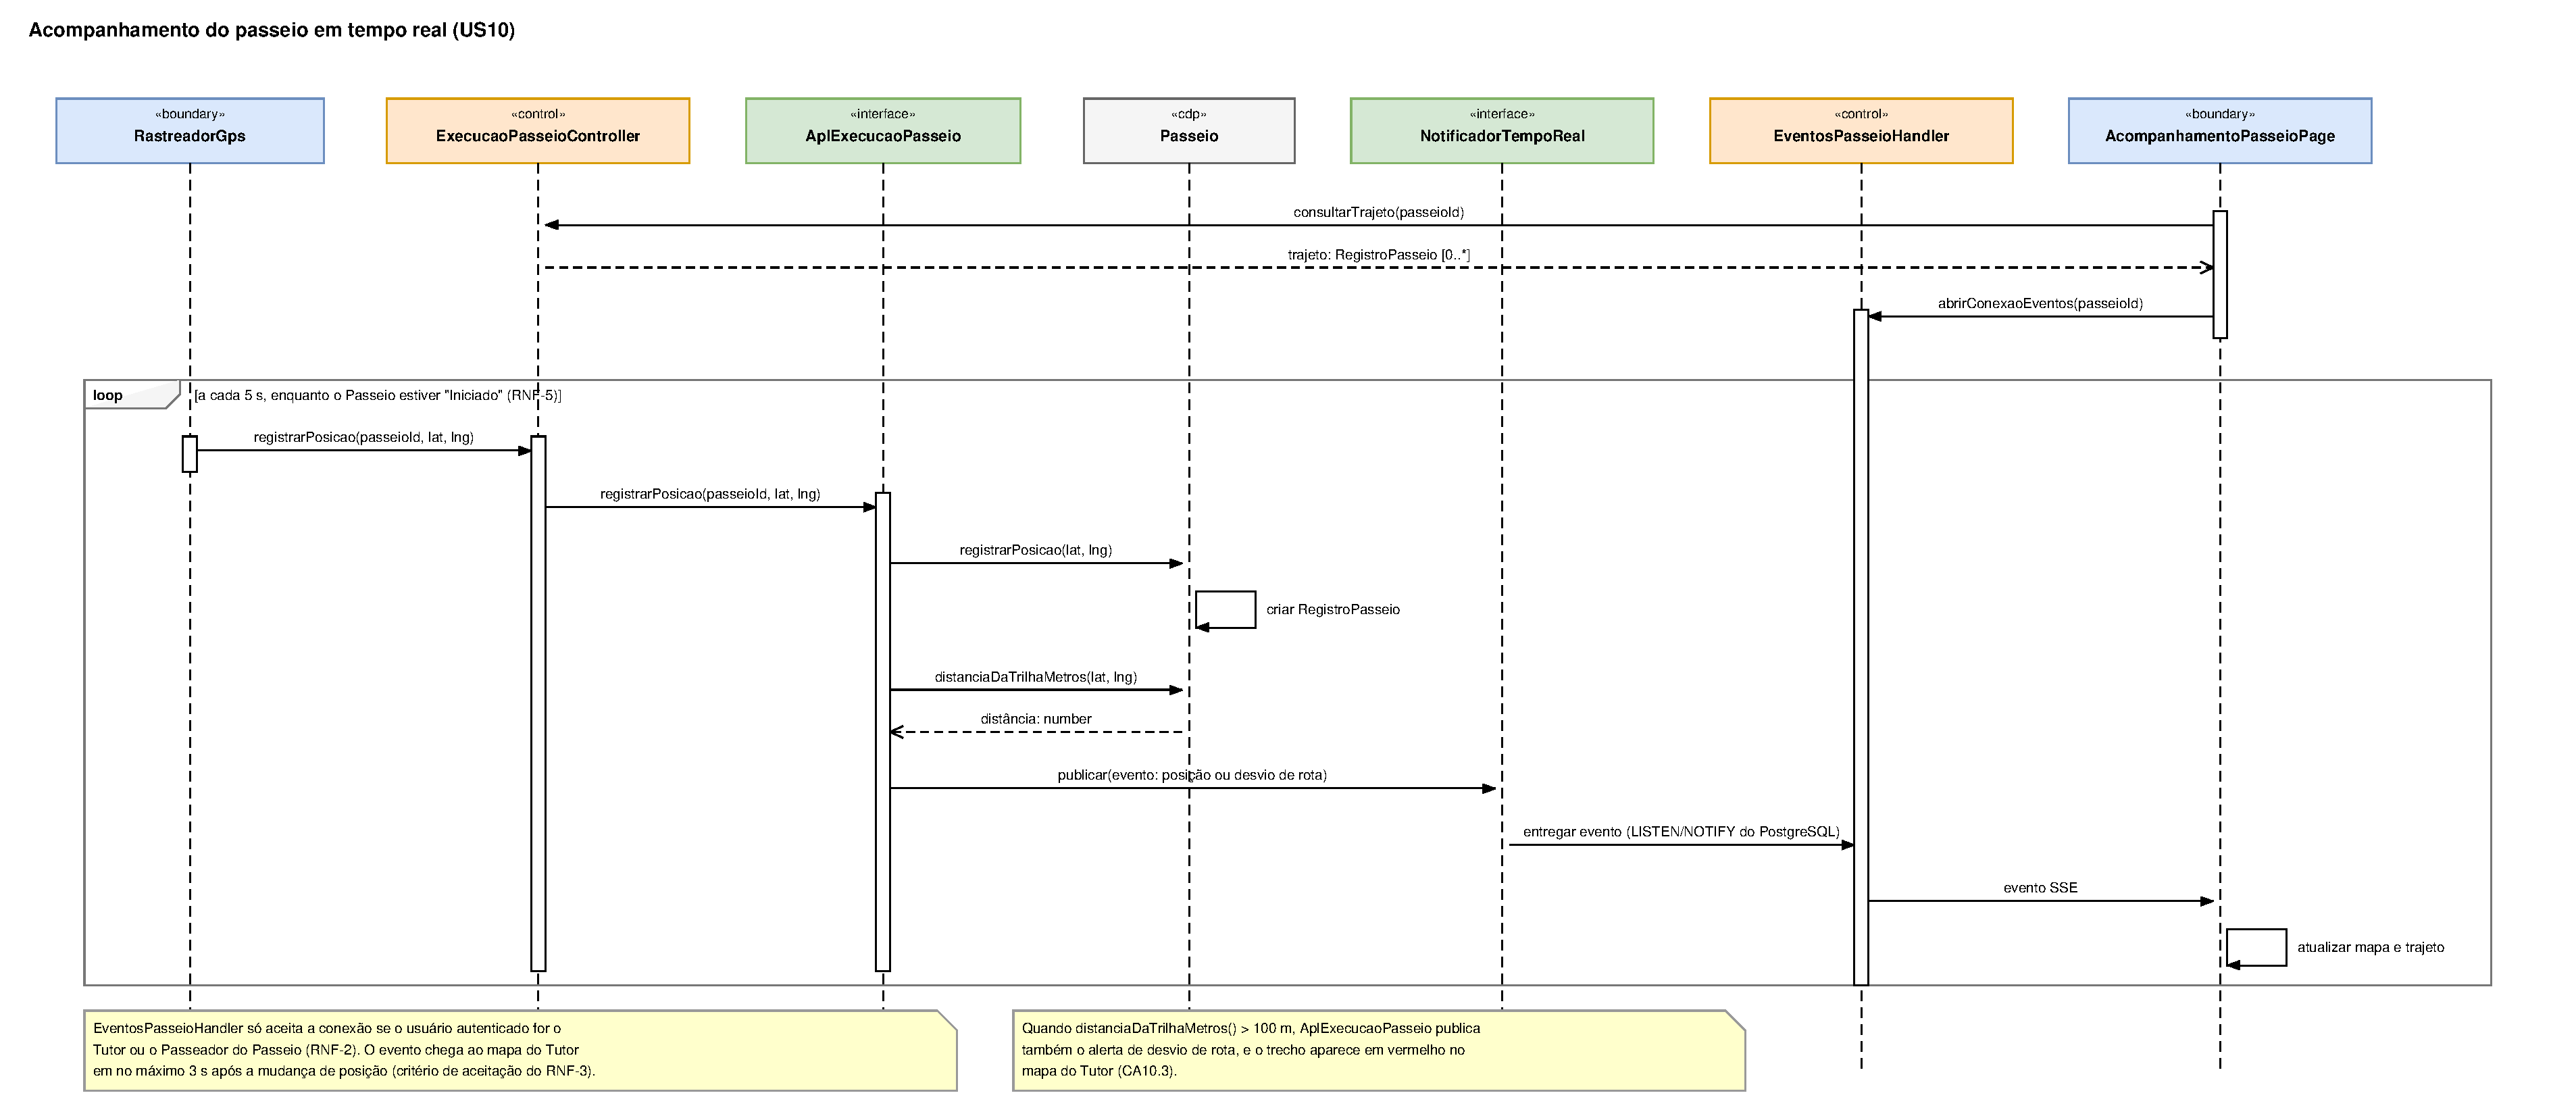
\includegraphics[angle=90,width=\textwidth,height=0.92\textheight,keepaspectratio]{figuras/ciu-servicos-seq-acompanhar.pdf}
	\caption{Diagrama de sequência do acompanhamento do passeio em tempo real.}
	\label{figura-ciu-seq-acompanhar}
\end{figure}


%=======================================================================================================
\FloatBarrier
\section{Subsistema Suporte}
\label{sec-ihc-suporte}

A Figura~\ref{figura-ciu-suporte} mostra o projeto da Camada de Interface com o Usuário do subsistema Suporte, juntamente com as classes de aplicação do \texttt{cgt} (Figura~\ref{figura-ln-suporte-cgt}). As telas correspondem às Figuras 25 a 30 do documento de requisitos. A Tabela~\ref{tabela-ciu-suporte} lista as páginas e os controladores.

\begin{figure}[h]
	\centering
	\figciu{figuras/ciu-suporte.png}{0.8}
	\caption{Projeto da Camada de Interface com o Usuário (\texttt{cih} e \texttt{cci}) do subsistema Suporte.}
	\label{figura-ciu-suporte}
\end{figure}

\begin{scriptsize}
\setlength{\tabcolsep}{3pt}
\begin{longtable}{|p{4.2cm}|p{3.6cm}|p{1.7cm}|p{1.3cm}|p{3.8cm}|}
	\caption{Páginas do subsistema Suporte.}
	\label{tabela-ciu-suporte}\\\hline
	\rowcolor{lightgray}
	\textbf{Página} & \textbf{Rota} & \textbf{Perfil} & \textbf{US} & \textbf{Controlador} \\\hline
	\endfirsthead
	\hline
	\rowcolor{lightgray}
	\textbf{Página} & \textbf{Rota} & \textbf{Perfil} & \textbf{US} & \textbf{Controlador} \\\hline
	\endhead
	\texttt{AbrirChamadoPage} & \texttt{/suporte/novo} & Tutor, Passeador & US16 & \texttt{Chamado\-Controller} \\\hline
	\texttt{MeusChamadosPage} & \texttt{/suporte} & Tutor, Passeador & US16 & \texttt{Chamado\-Controller} \\\hline
	\texttt{DetalheChamadoPage} & \texttt{/suporte/\allowbreak [protocolo]} & Tutor, Passeador & US16 & \texttt{Chamado\-Controller} e \texttt{EventosSuporte\-Handler} \\\hline
	\texttt{FilaAtendimentoPage} & \texttt{/atendimento/\allowbreak chamados} & Atendente & US17 & \texttt{Atendimento\-Controller} e \texttt{EventosSuporte\-Handler} \\\hline
	\texttt{AtendimentoChamadoPage} & \texttt{/atendimento/\allowbreak chamados/[id]} & Atendente & US17 & \texttt{Atendimento\-Controller} \\\hline
\end{longtable}
\end{scriptsize}

\begin{sloppypar}
\texttt{ChamadoController} se liga a \texttt{AplChamado}, e \texttt{AtendimentoController} a \texttt{AplAtendimento}. \texttt{EventosSuporteHandler} é um \textit{Route Handler} que, como \texttt{EventosPasseioHandler}, não chama operações do \texttt{cgt}: ele só assina os eventos que \texttt{AplChamado} e \texttt{AplAtendimento} publicam em \texttt{NotificadorTempoReal} e os repassa por SSE às páginas abertas. As funcionalidades do subsistema são:

\begin{itemize}
	\item \textbf{Abertura de chamado:} \texttt{AbrirChamadoPage} pede o tipo do problema (lista de seleção), a descrição, os anexos (fotos e capturas de tela) e, quando o problema aconteceu em um passeio, o passeio relacionado. Os dados vão a \texttt{ChamadoController}, que chama \texttt{abrirChamado()}. O tipo e a descrição são obrigatórios (CA16.1). Em caso de sucesso, o controlador redireciona para \texttt{DetalheChamadoPage}, que mostra o protocolo gerado e o status ``Em análise'' (CA16.2). Para chamados de ``Emergência'', a página destaca o tipo, e \texttt{AplChamado} publica o evento em \texttt{NotificadorTempoReal}, que o leva à fila do Atendente. \texttt{MeusChamadosPage} tem um \textit{link} para esta página;
	\item \textbf{Consulta dos chamados:} \texttt{MeusChamadosPage} lista os chamados do usuário (\texttt{listarMeusChamados()}), com protocolo, tipo e status. Ao escolher um deles, \texttt{DetalheChamadoPage} mostra o chamado e as respostas do Atendente (\texttt{consultarChamado()}). Quando o Atendente responde, \texttt{AplAtendimento} publica o evento em \texttt{NotificadorTempoReal}, e \texttt{DetalheChamadoPage}, conectada a \texttt{EventosSuporteHandler}, mostra a resposta sem recarregar a página (CA16.3);
	\item \textbf{Fila de atendimento:} \texttt{FilaAtendimentoPage} lista os chamados abertos (\texttt{listarFilaAtendimento()}), com os de ``Emergência'' em destaque e no topo, e mostra para cada um o tempo de espera. A página também mostra o indicador de primeiro atendimento em até 30 minutos (\texttt{calcularIndicadorAtendimento()}, RNF-4). A página recebe novos chamados por \texttt{EventosSuporteHandler}, sem o Atendente precisar recarregá-la;
	\item \textbf{Atendimento do chamado:} \texttt{AtendimentoChamadoPage} mostra (\texttt{consultarChamado()}) a descrição, o passeio relacionado, os anexos (que o Atendente pode visualizar ou baixar, CA17.3) e as respostas anteriores. O Atendente escreve a resposta (\texttt{responderChamado()}), o que muda o status para ``Em atendimento'', e pode encerrar o chamado com confirmação (\texttt{encerrarChamado()}), mudando o status para ``Resolvido''. Depois de responder, o Atendente continua na própria página; depois de encerrar, o controlador volta para \texttt{FilaAtendimentoPage}.
\end{itemize}
\end{sloppypar}


%=======================================================================================================
\FloatBarrier
\section{Padrões de Projeto na Camada de Apresentação}
\label{sec-ihc-padroes}

Além do MVC, foram usados padrões de projeto~\cite{falbo:notas18} na Camada de Apresentação:

\begin{itemize}
	\item \textbf{Observador (\textit{Observer}):} as páginas de acompanhamento do passeio, de fila de atendimento e de chamados são observadoras dos eventos publicados por \texttt{NotificadorTempoReal}. O navegador se inscreve por meio de um \texttt{EventSource}, conectado a \texttt{EventosPasseioHandler} ou a \texttt{EventosSuporteHandler}, e é avisado das mudanças, em vez de consultar o servidor de tempos em tempos (RNF-3);
	\item \textbf{Decorador (\textit{Decorator}):} os \textit{layouts} do Next.js envolvem as páginas de cada área (Tutor, Passeador e Atendente) com o menu, o cabeçalho e a verificação de sessão e de perfil, de modo que a estrutura visual e o controle de acesso não são repetidos em cada página;
	\item \textbf{Comando (\textit{Command}):} cada \textit{Server Action} representa um comando do usuário (por exemplo, agendar, cancelar, aceitar, responder), recebe os dados do formulário e devolve o resultado da operação, o que mantém um controlador pequeno e focado em uma tarefa.
\end{itemize}
\endgroup



%%% Páginas finais do documento: bibliografia e anexos. %%%
% Finaliza a parte no bookmark do PDF para que se inicie o bookmark na raiz e adiciona espaço de parte no sumário.
\phantompart

% Marca o início dos elementos pós-textuais.
\postextual

% Referências bibliográficas
\bibliography{bibliografia}

% Índice remissivo.
\phantompart
\printindex

% Fim do documento.
\end{document}
